% Options for packages loaded elsewhere
\PassOptionsToPackage{unicode}{hyperref}
\PassOptionsToPackage{hyphens}{url}
\PassOptionsToPackage{dvipsnames,svgnames,x11names}{xcolor}
%
\documentclass[
  letterpaper,
  DIV=11,
  numbers=noendperiod]{scrartcl}

\usepackage{amsmath,amssymb}
\usepackage{iftex}
\ifPDFTeX
  \usepackage[T1]{fontenc}
  \usepackage[utf8]{inputenc}
  \usepackage{textcomp} % provide euro and other symbols
\else % if luatex or xetex
  \usepackage{unicode-math}
  \defaultfontfeatures{Scale=MatchLowercase}
  \defaultfontfeatures[\rmfamily]{Ligatures=TeX,Scale=1}
\fi
\usepackage{lmodern}
\ifPDFTeX\else  
    % xetex/luatex font selection
\fi
% Use upquote if available, for straight quotes in verbatim environments
\IfFileExists{upquote.sty}{\usepackage{upquote}}{}
\IfFileExists{microtype.sty}{% use microtype if available
  \usepackage[]{microtype}
  \UseMicrotypeSet[protrusion]{basicmath} % disable protrusion for tt fonts
}{}
\makeatletter
\@ifundefined{KOMAClassName}{% if non-KOMA class
  \IfFileExists{parskip.sty}{%
    \usepackage{parskip}
  }{% else
    \setlength{\parindent}{0pt}
    \setlength{\parskip}{6pt plus 2pt minus 1pt}}
}{% if KOMA class
  \KOMAoptions{parskip=half}}
\makeatother
\usepackage{xcolor}
\usepackage{soul}
\setlength{\emergencystretch}{3em} % prevent overfull lines
\setcounter{secnumdepth}{-\maxdimen} % remove section numbering
% Make \paragraph and \subparagraph free-standing
\ifx\paragraph\undefined\else
  \let\oldparagraph\paragraph
  \renewcommand{\paragraph}[1]{\oldparagraph{#1}\mbox{}}
\fi
\ifx\subparagraph\undefined\else
  \let\oldsubparagraph\subparagraph
  \renewcommand{\subparagraph}[1]{\oldsubparagraph{#1}\mbox{}}
\fi

\usepackage{color}
\usepackage{fancyvrb}
\newcommand{\VerbBar}{|}
\newcommand{\VERB}{\Verb[commandchars=\\\{\}]}
\DefineVerbatimEnvironment{Highlighting}{Verbatim}{commandchars=\\\{\}}
% Add ',fontsize=\small' for more characters per line
\usepackage{framed}
\definecolor{shadecolor}{RGB}{241,243,245}
\newenvironment{Shaded}{\begin{snugshade}}{\end{snugshade}}
\newcommand{\AlertTok}[1]{\textcolor[rgb]{0.68,0.00,0.00}{#1}}
\newcommand{\AnnotationTok}[1]{\textcolor[rgb]{0.37,0.37,0.37}{#1}}
\newcommand{\AttributeTok}[1]{\textcolor[rgb]{0.40,0.45,0.13}{#1}}
\newcommand{\BaseNTok}[1]{\textcolor[rgb]{0.68,0.00,0.00}{#1}}
\newcommand{\BuiltInTok}[1]{\textcolor[rgb]{0.00,0.23,0.31}{#1}}
\newcommand{\CharTok}[1]{\textcolor[rgb]{0.13,0.47,0.30}{#1}}
\newcommand{\CommentTok}[1]{\textcolor[rgb]{0.37,0.37,0.37}{#1}}
\newcommand{\CommentVarTok}[1]{\textcolor[rgb]{0.37,0.37,0.37}{\textit{#1}}}
\newcommand{\ConstantTok}[1]{\textcolor[rgb]{0.56,0.35,0.01}{#1}}
\newcommand{\ControlFlowTok}[1]{\textcolor[rgb]{0.00,0.23,0.31}{#1}}
\newcommand{\DataTypeTok}[1]{\textcolor[rgb]{0.68,0.00,0.00}{#1}}
\newcommand{\DecValTok}[1]{\textcolor[rgb]{0.68,0.00,0.00}{#1}}
\newcommand{\DocumentationTok}[1]{\textcolor[rgb]{0.37,0.37,0.37}{\textit{#1}}}
\newcommand{\ErrorTok}[1]{\textcolor[rgb]{0.68,0.00,0.00}{#1}}
\newcommand{\ExtensionTok}[1]{\textcolor[rgb]{0.00,0.23,0.31}{#1}}
\newcommand{\FloatTok}[1]{\textcolor[rgb]{0.68,0.00,0.00}{#1}}
\newcommand{\FunctionTok}[1]{\textcolor[rgb]{0.28,0.35,0.67}{#1}}
\newcommand{\ImportTok}[1]{\textcolor[rgb]{0.00,0.46,0.62}{#1}}
\newcommand{\InformationTok}[1]{\textcolor[rgb]{0.37,0.37,0.37}{#1}}
\newcommand{\KeywordTok}[1]{\textcolor[rgb]{0.00,0.23,0.31}{#1}}
\newcommand{\NormalTok}[1]{\textcolor[rgb]{0.00,0.23,0.31}{#1}}
\newcommand{\OperatorTok}[1]{\textcolor[rgb]{0.37,0.37,0.37}{#1}}
\newcommand{\OtherTok}[1]{\textcolor[rgb]{0.00,0.23,0.31}{#1}}
\newcommand{\PreprocessorTok}[1]{\textcolor[rgb]{0.68,0.00,0.00}{#1}}
\newcommand{\RegionMarkerTok}[1]{\textcolor[rgb]{0.00,0.23,0.31}{#1}}
\newcommand{\SpecialCharTok}[1]{\textcolor[rgb]{0.37,0.37,0.37}{#1}}
\newcommand{\SpecialStringTok}[1]{\textcolor[rgb]{0.13,0.47,0.30}{#1}}
\newcommand{\StringTok}[1]{\textcolor[rgb]{0.13,0.47,0.30}{#1}}
\newcommand{\VariableTok}[1]{\textcolor[rgb]{0.07,0.07,0.07}{#1}}
\newcommand{\VerbatimStringTok}[1]{\textcolor[rgb]{0.13,0.47,0.30}{#1}}
\newcommand{\WarningTok}[1]{\textcolor[rgb]{0.37,0.37,0.37}{\textit{#1}}}

\providecommand{\tightlist}{%
  \setlength{\itemsep}{0pt}\setlength{\parskip}{0pt}}\usepackage{longtable,booktabs,array}
\usepackage{calc} % for calculating minipage widths
% Correct order of tables after \paragraph or \subparagraph
\usepackage{etoolbox}
\makeatletter
\patchcmd\longtable{\par}{\if@noskipsec\mbox{}\fi\par}{}{}
\makeatother
% Allow footnotes in longtable head/foot
\IfFileExists{footnotehyper.sty}{\usepackage{footnotehyper}}{\usepackage{footnote}}
\makesavenoteenv{longtable}
\usepackage{graphicx}
\makeatletter
\def\maxwidth{\ifdim\Gin@nat@width>\linewidth\linewidth\else\Gin@nat@width\fi}
\def\maxheight{\ifdim\Gin@nat@height>\textheight\textheight\else\Gin@nat@height\fi}
\makeatother
% Scale images if necessary, so that they will not overflow the page
% margins by default, and it is still possible to overwrite the defaults
% using explicit options in \includegraphics[width, height, ...]{}
\setkeys{Gin}{width=\maxwidth,height=\maxheight,keepaspectratio}
% Set default figure placement to htbp
\makeatletter
\def\fps@figure{htbp}
\makeatother

\KOMAoption{captions}{tableheading}
\makeatletter
\makeatother
\makeatletter
\makeatother
\makeatletter
\@ifpackageloaded{caption}{}{\usepackage{caption}}
\AtBeginDocument{%
\ifdefined\contentsname
  \renewcommand*\contentsname{Table of contents}
\else
  \newcommand\contentsname{Table of contents}
\fi
\ifdefined\listfigurename
  \renewcommand*\listfigurename{List of Figures}
\else
  \newcommand\listfigurename{List of Figures}
\fi
\ifdefined\listtablename
  \renewcommand*\listtablename{List of Tables}
\else
  \newcommand\listtablename{List of Tables}
\fi
\ifdefined\figurename
  \renewcommand*\figurename{Figure}
\else
  \newcommand\figurename{Figure}
\fi
\ifdefined\tablename
  \renewcommand*\tablename{Table}
\else
  \newcommand\tablename{Table}
\fi
}
\@ifpackageloaded{float}{}{\usepackage{float}}
\floatstyle{ruled}
\@ifundefined{c@chapter}{\newfloat{codelisting}{h}{lop}}{\newfloat{codelisting}{h}{lop}[chapter]}
\floatname{codelisting}{Listing}
\newcommand*\listoflistings{\listof{codelisting}{List of Listings}}
\makeatother
\makeatletter
\@ifpackageloaded{caption}{}{\usepackage{caption}}
\@ifpackageloaded{subcaption}{}{\usepackage{subcaption}}
\makeatother
\makeatletter
\@ifpackageloaded{tcolorbox}{}{\usepackage[skins,breakable]{tcolorbox}}
\makeatother
\makeatletter
\@ifundefined{shadecolor}{\definecolor{shadecolor}{rgb}{.97, .97, .97}}
\makeatother
\makeatletter
\makeatother
\makeatletter
\makeatother
\ifLuaTeX
  \usepackage{selnolig}  % disable illegal ligatures
\fi
\IfFileExists{bookmark.sty}{\usepackage{bookmark}}{\usepackage{hyperref}}
\IfFileExists{xurl.sty}{\usepackage{xurl}}{} % add URL line breaks if available
\urlstyle{same} % disable monospaced font for URLs
\hypersetup{
  pdftitle={Report pdf},
  colorlinks=true,
  linkcolor={blue},
  filecolor={Maroon},
  citecolor={Blue},
  urlcolor={Blue},
  pdfcreator={LaTeX via pandoc}}

\title{Report pdf}
\author{}
\date{}

\begin{document}
\maketitle
\ifdefined\Shaded\renewenvironment{Shaded}{\begin{tcolorbox}[frame hidden, boxrule=0pt, interior hidden, sharp corners, breakable, enhanced, borderline west={3pt}{0pt}{shadecolor}]}{\end{tcolorbox}}\fi

There are two common workflows for data integration: ELT(Extract, Load,
Transform) and ETL (Extract, Transform, Load)

The major difference between ELT and ETL is that in the ELT stage,
normalization is performed after the datasets are imported into the
database. In the ETL stage, the data is normalized and transformed
before it is loaded into the database.

In our work, we chose ETL (Extract, Transform, Load) instead of ELT as
our workflow and used SQL and R interchangeably to perform
transformations. This is because we have found that ETL workflow is more
suitable for small data sets, so we thought that it would be more
compromised with our work.

\hypertarget{part-1-database-design-and-implementation}{%
\subsection{Part 1: Database Design and
Implementation}\label{part-1-database-design-and-implementation}}

\hypertarget{task-1.1-e-r-diagram}{%
\subsubsection{Task 1.1: E-R Diagram}\label{task-1.1-e-r-diagram}}

\hypertarget{entities}{%
\paragraph{Entities}\label{entities}}

Our E-R Diagram for an E-commerce database consisted of five main
entities:

\begin{enumerate}
\def\labelenumi{\arabic{enumi}.}
\tightlist
\item
  CUSTOMER: Represents details of individuals or entities who purchase
  products, including attributes such as customer ID, customer name,
  contact information, and gender.~
\item
  PRODUCT: Represents details of items available for sale, including
  attributes such as product ID, product name, description, rating,
  price, and available stock.~
\item
  ADVERTISEMENT: Represents details of promotional activities used to
  advertise products, including attributes such as advertisement ID,
  number of times the advertisement is shown, cost of the advertisement,
  and the place the advertisement was placed.~
\item
  SUPPLIER: Represents details of entities providing products to
  businesses or customers, including attributes such as supplier ID,
  supplier name, and contact information.~
\item
  CATEGORY: Represents product classifications or groupings, including
  attributes such as category unique ID, name, and fee amount as a
  percentage.
\end{enumerate}

\hypertarget{relationships}{%
\paragraph{Relationships}\label{relationships}}

The relationships among these entities are as follows:~

\begin{itemize}
\item
  CUSTOMER and PRODUCT have an M-N relationship meaning one customer can
  order many products, and one product can be ordered by many customers.

  The relationship is shown as ORDER, representing a customer placing an
  order to purchase products. It also contains some attributes to store
  the details of each order, including order ID, order date, order
  status, order quantity, promo code, payment method, and delivery fee.

  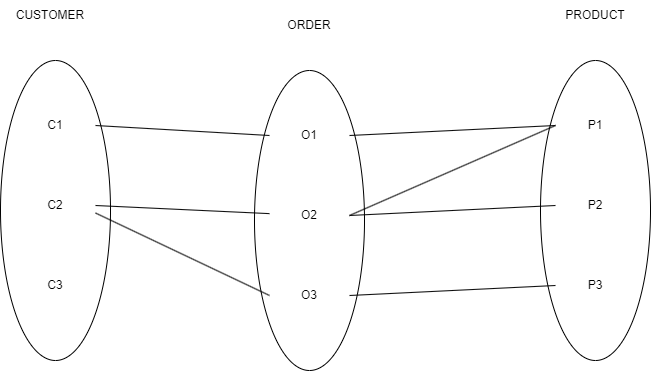
\includegraphics[width=4.875in,height=\textheight]{images/Customer-Product relationship.drawio.png}
\item
  PRODUCT has a self-referencing relationship of 1 to many. The
  relationship is shown as Sold\_Together, indicating that one product
  can be sold together with others as a bundle.

  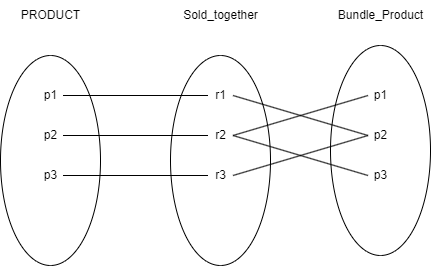
\includegraphics{images/Product Self-reference Relationship.drawio.png}
\item
  PRODUCT and ADVERTISEMENT have an M-N relationship. This relationship
  is shown as ADVERTISE\_IN to reflect products presented in the
  advertisements, meaning multiple advertisements can promote one
  product, and one advertisement can promote multiple products.~

  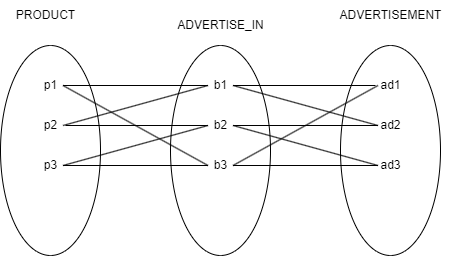
\includegraphics{images/Product-Advertisement relationship.drawio.png}
\item
  PRODUCT and SUPPLIER have an N-1 relationship, indicating that one
  product can be supplied by only one supplier, but one supplier can
  provide multiple products.~

  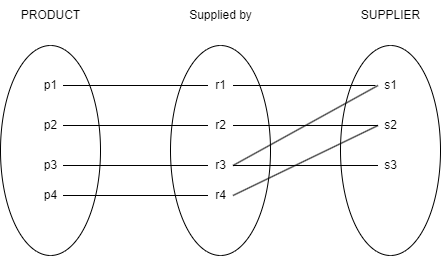
\includegraphics{images/Product-Supplier relationship.drawio.png}
\item
  CATEGORY and PRODUCT have an 1-N relationship, meaning one product can
  belong to only one category, but one category can contain multiple
  products.~

  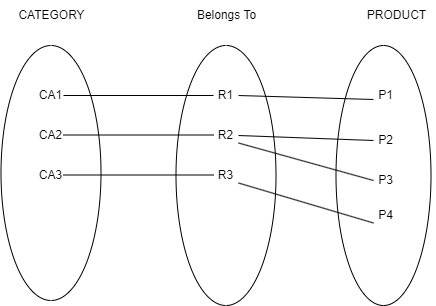
\includegraphics{images/Category-Product Relationship.drawio (1).png}
\end{itemize}

As a result, this is our E-R diagram.

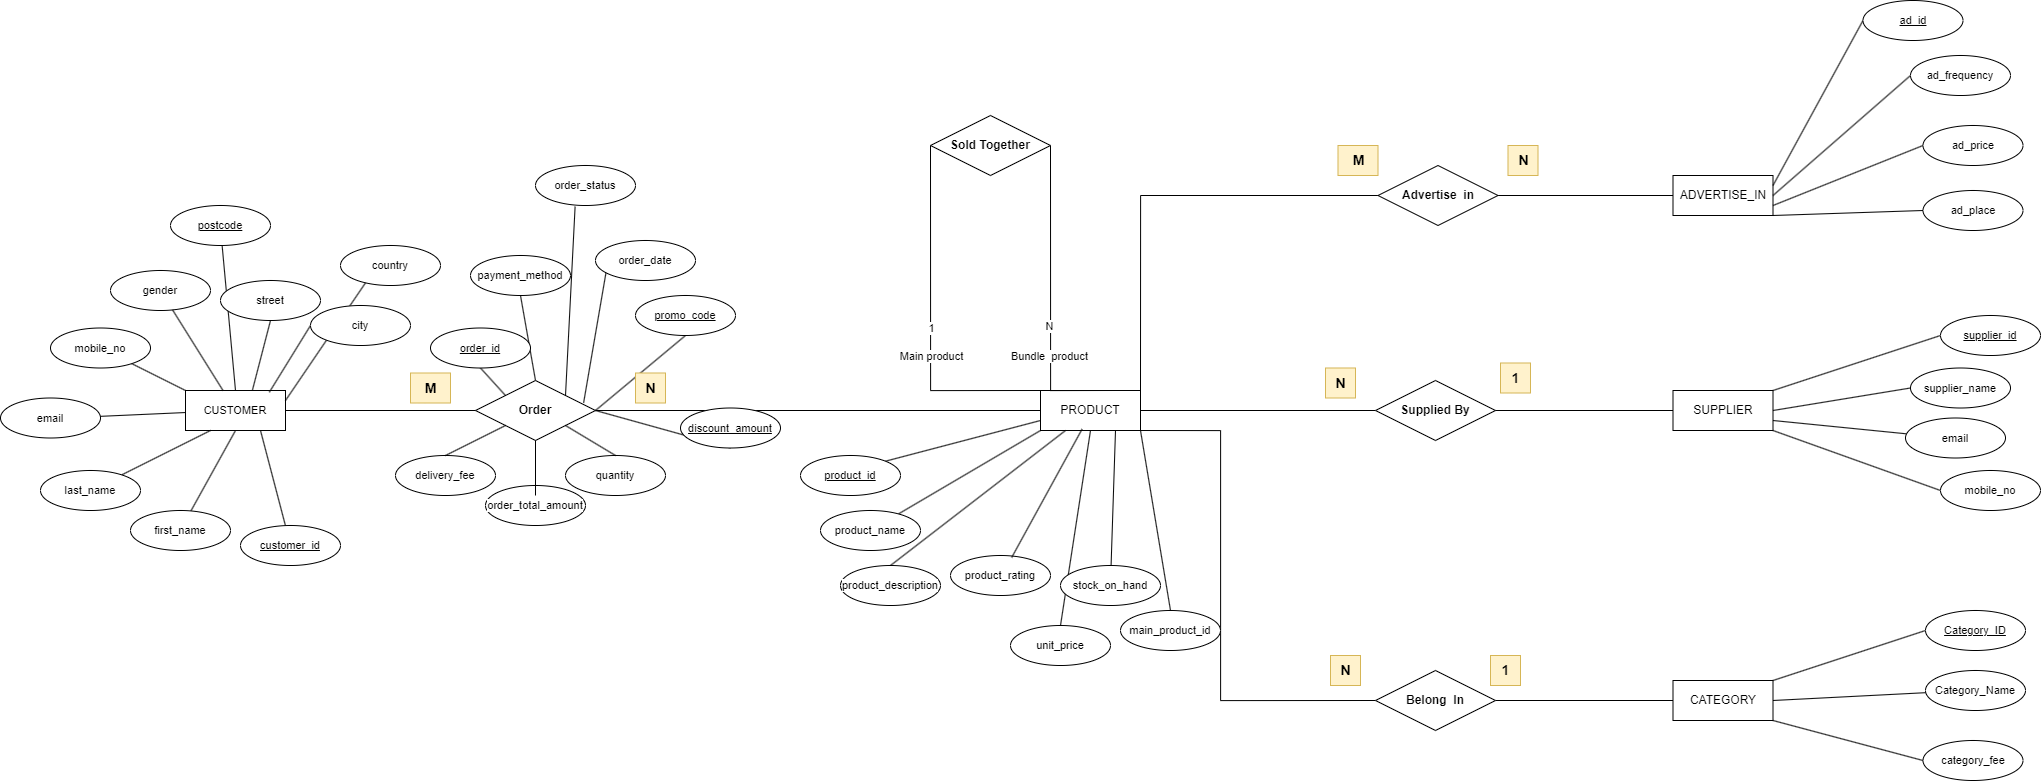
\includegraphics{images/E-R Diagram(Final)-Before Final.drawio.png}

\hypertarget{task-1.2-sql-database-schema-creation}{%
\subsubsection{Task 1.2: SQL Database Schema
Creation}\label{task-1.2-sql-database-schema-creation}}

\hypertarget{normalization}{%
\paragraph{Normalization:}\label{normalization}}

According to our first draft of the E-R diagram, two main adjustments
were made in order to comply with 3NF

The first adjustment was on the ORDER table. After reviewing the order
of normal forms, it was found that the ORDER entity still did not comply
with 3NF.

Functional Dependency:

\{order\_id, customer\_id, product\_id \} -\textgreater{} \{ order\_date
, order\_status, order\_quantity, promo\_code, discount amount,
payment\_method, delivery\_fee\}

\{promo\_code\} -\textgreater{} \{ discount\_amount\}

As we assumed that order\_id could be duplicated to represent products
ordered by the same customer simultaneously, there would be UPDATE
anomalies. If there is an update on any attributes, such as
payment\_methods, we must alter more than one row in case there is more
than one product in that order\_id. In addition, discount\_amount is
also transitively dependent on promo\_code.

Therefore, we separated the ORDER table into three entities including:

\begin{enumerate}
\def\labelenumi{\arabic{enumi}.}
\tightlist
\item
  ORDER\_DETAIL is similar to the ORDER table but has fewer attributes
  to contain each order's details. It has product\_id as a primary key,
  customer\_id and promo\_code as foreign keys, and other attributes
  like order\_date, order\_status, and payment\_method.
\item
  ORDER\_ITEM contains product IDs and the quantities ordered in each
  order. The table has order\_id and product\_id as foreign keys and a
  composite primary key, and quantity as another attribute.
\item
  DISCOUNT is created to store the data of available promotional
  discounts, which consists of promo\_code as a primary key and
  discount\_amount.
\end{enumerate}

The next adjustment was on the CUSTOMER table, which was initially on
2NF. Based on its function dependency, street, city, and country can
also be determined by postcode and customer\_id.

Functional Dependency:

\{customer\_id\} -\textgreater\{ first\_name , last\_name , gender ,
email, mobile\_no , street , city , country , postcode \} \{postcode\}
-\textgreater{} \{ street, city , country \}

This indicated that street, city, and country were transitively
dependent on postcode. As a result, a new table is created as ADDRESS,
which has postcode as a primary key and stores street, city, and country
as other attributes.

In summary, four new entities were created from the normalization, which
were ORDER\_DETAIL, ORDER\_ITEM, DISCOUNT, and ADDRESS. This resulted in
a total of ten entities in our schema.

\textbf{Logical Schema}

According to the E-R diagram and normalization s, we can list the
logical schema as follows:

\begin{itemize}
\item
  CUSTOMER(\ul{customer\_id}, first\_name, last\_name, gender, email,
  mobile\_no, address\_id)
\item
  ADDRESS(\ul{address\_id}, postcode, street, city, country)
\item
  DISCOUNT(\ul{promo\_code}, discount\_amount)
\item
  ADVERTISEMENT(\ul{ad\_id}, ad\_frequency, ad\_place, ad\_price)~
\item
  SUPPLIER(\ul{supplier\_id}, supplier\_name, email, mobile\_no)~
\item
  CATEGORY(\ul{category\_id,} category\_name, category\_fee)
\item
  PRODUCT(\ul{product\_id}, product\_name, product\_description,
  product\_rating, unit\_price, stock\_at\_hand, main\_product\_id,
  category\_id, supplier\_id)~
\item
  ORDER\_DETAIL(\ul{order\_id,} customer\_id, order\_date,
  order\_status, promo\_code, payment\_method, delivery\_fee)
\item
  ORDER\_ITEM(\ul{order\_id}, product\_id, quantity)
\item
  ADVERTISE\_IN(\ul{product\_id}, ad\_id)
\end{itemize}

\hypertarget{physical-schema-update}{%
\paragraph{Physical Schema
\textless update\textgreater{}}\label{physical-schema-update}}

\begin{verbatim}
Warning: package 'RSQLite' was built under R version 4.3.2
\end{verbatim}

\begin{verbatim}

Attaching package: 'dplyr'
\end{verbatim}

\begin{verbatim}
The following objects are masked from 'package:stats':

    filter, lag
\end{verbatim}

\begin{verbatim}
The following objects are masked from 'package:base':

    intersect, setdiff, setequal, union
\end{verbatim}

\begin{verbatim}

Attaching package: 'gridExtra'
\end{verbatim}

\begin{verbatim}
The following object is masked from 'package:dplyr':

    combine
\end{verbatim}

\begin{verbatim}
Warning: package 'ggplot2' was built under R version 4.3.3
\end{verbatim}

Firstly, we created a connection to our database named ``database.db''

\begin{Shaded}
\begin{Highlighting}[]
\NormalTok{connect }\OtherTok{\textless{}{-}} \FunctionTok{dbConnect}\NormalTok{(RSQLite}\SpecialCharTok{::}\FunctionTok{SQLite}\NormalTok{(), }\StringTok{"database.db"}\NormalTok{)}
\end{Highlighting}
\end{Shaded}

Then, we first created parent entities, including CUSTOMER, DISCOUNT,
ADVERTISEMENT, SUPPLIER, and CATEGORY.

\begin{enumerate}
\def\labelenumi{\arabic{enumi}.}
\item
  Create CUSTOMER entity

\begin{Shaded}
\begin{Highlighting}[]
\KeywordTok{CREATE} \KeywordTok{TABLE} \ControlFlowTok{IF} \KeywordTok{NOT} \KeywordTok{EXISTS}\NormalTok{ CUSTOMER (}
\NormalTok{  customer\_id }\DataTypeTok{VARCHAR}\NormalTok{(}\DecValTok{50}\NormalTok{) }\KeywordTok{PRIMARY} \KeywordTok{KEY}\NormalTok{, }
\NormalTok{  first\_name }\DataTypeTok{VARCHAR}\NormalTok{(}\DecValTok{50}\NormalTok{) }\KeywordTok{NOT} \KeywordTok{NULL}\NormalTok{,}
\NormalTok{  last\_name }\DataTypeTok{VARCHAR}\NormalTok{(}\DecValTok{50}\NormalTok{) }\KeywordTok{NOT} \KeywordTok{NULL}\NormalTok{,}
\NormalTok{  gender }\DataTypeTok{VARCHAR}\NormalTok{(}\DecValTok{10}\NormalTok{),}
\NormalTok{  customer\_email }\DataTypeTok{VARCHAR}\NormalTok{(}\DecValTok{50}\NormalTok{) }\KeywordTok{NOT} \KeywordTok{NULL} \KeywordTok{UNIQUE}\NormalTok{,}
\NormalTok{  customer\_mobile }\DataTypeTok{VARCHAR}\NormalTok{(}\DecValTok{15}\NormalTok{) }\KeywordTok{NOT} \KeywordTok{NULL} \KeywordTok{UNIQUE}\NormalTok{,}
\NormalTok{  address\_id }\DataTypeTok{VARCHAR}\NormalTok{(}\DecValTok{50}\NormalTok{) }\KeywordTok{NOT} \KeywordTok{NULL}\NormalTok{,}
  \KeywordTok{FOREIGN} \KeywordTok{KEY}\NormalTok{ (address\_id) }\KeywordTok{REFERENCES}\NormalTok{ ADDRESS (address\_id)}
\NormalTok{);}
\end{Highlighting}
\end{Shaded}
\item
  Create ADDRESS entity

\begin{Shaded}
\begin{Highlighting}[]
\KeywordTok{CREATE} \KeywordTok{TABLE} \ControlFlowTok{IF} \KeywordTok{NOT} \KeywordTok{EXISTS}\NormalTok{ ADDRESS (}
\NormalTok{  address\_id }\DataTypeTok{VARCHAR}\NormalTok{(}\DecValTok{50}\NormalTok{) }\KeywordTok{PRIMARY} \KeywordTok{KEY}\NormalTok{,}
\NormalTok{  postcode }\DataTypeTok{VARCHAR}\NormalTok{(}\DecValTok{20}\NormalTok{) }\KeywordTok{NOT} \KeywordTok{NULL}\NormalTok{, }
\NormalTok{  street }\DataTypeTok{VARCHAR}\NormalTok{(}\DecValTok{50}\NormalTok{) }\KeywordTok{NOT} \KeywordTok{NULL}\NormalTok{,}
\NormalTok{  city }\DataTypeTok{VARCHAR}\NormalTok{(}\DecValTok{100}\NormalTok{) }\KeywordTok{NOT} \KeywordTok{NULL}\NormalTok{,}
\NormalTok{  country }\DataTypeTok{VARCHAR}\NormalTok{(}\DecValTok{100}\NormalTok{) }\KeywordTok{NOT} \KeywordTok{NULL}
\NormalTok{  );}
\end{Highlighting}
\end{Shaded}
\item
  Create DISCOUNT entity

\begin{Shaded}
\begin{Highlighting}[]
\KeywordTok{CREATE} \KeywordTok{TABLE} \ControlFlowTok{IF} \KeywordTok{NOT} \KeywordTok{EXISTS}\NormalTok{ DISCOUNT (}
\NormalTok{  promo\_code }\DataTypeTok{VARCHAR}\NormalTok{(}\DecValTok{20}\NormalTok{) }\KeywordTok{PRIMARY} \KeywordTok{KEY}\NormalTok{, }
\NormalTok{  discount\_percent }\DataTypeTok{INT} \KeywordTok{NOT} \KeywordTok{NULL}
\NormalTok{);}
\end{Highlighting}
\end{Shaded}
\item
  Create ADVERTISEMENT entity

\begin{Shaded}
\begin{Highlighting}[]
\KeywordTok{CREATE} \KeywordTok{TABLE} \ControlFlowTok{IF} \KeywordTok{NOT} \KeywordTok{EXISTS}\NormalTok{ ADVERTISEMENT (}
\NormalTok{  ad\_id }\DataTypeTok{VARCHAR}\NormalTok{(}\DecValTok{50}\NormalTok{) }\KeywordTok{PRIMARY} \KeywordTok{KEY}\NormalTok{, }
\NormalTok{  ad\_frequency }\DataTypeTok{INT} \KeywordTok{NOT} \KeywordTok{NULL}\NormalTok{,}
\NormalTok{  ad\_place }\DataTypeTok{VARCHAR}\NormalTok{(}\DecValTok{50}\NormalTok{) }\KeywordTok{NOT} \KeywordTok{NULL}\NormalTok{,}
\NormalTok{  ad\_price }\DataTypeTok{DECIMAL}\NormalTok{(}\DecValTok{10}\NormalTok{, }\DecValTok{2}\NormalTok{) }\KeywordTok{NOT} \KeywordTok{NULL}
\NormalTok{);}
\end{Highlighting}
\end{Shaded}
\item
  Create SUPPLIER entity

\begin{Shaded}
\begin{Highlighting}[]
\KeywordTok{CREATE} \KeywordTok{TABLE} \ControlFlowTok{IF} \KeywordTok{NOT} \KeywordTok{EXISTS}\NormalTok{ SUPPLIER (}
\NormalTok{  supplier\_id }\DataTypeTok{VARCHAR}\NormalTok{(}\DecValTok{250}\NormalTok{) }\KeywordTok{PRIMARY} \KeywordTok{KEY}\NormalTok{, }
\NormalTok{  supplier\_name }\DataTypeTok{VARCHAR}\NormalTok{(}\DecValTok{250}\NormalTok{) }\KeywordTok{NOT} \KeywordTok{NULL}\NormalTok{,}
\NormalTok{  supplier\_email }\DataTypeTok{VARCHAR}\NormalTok{(}\DecValTok{250}\NormalTok{) }\KeywordTok{NOT} \KeywordTok{NULL}\NormalTok{,}
\NormalTok{  supplier\_mobile }\DataTypeTok{VARCHAR}\NormalTok{(}\DecValTok{20}\NormalTok{) }\KeywordTok{NOT} \KeywordTok{NULL}
\NormalTok{);}
\end{Highlighting}
\end{Shaded}
\item
  Create CATEGORY entity

\begin{Shaded}
\begin{Highlighting}[]
\KeywordTok{CREATE} \KeywordTok{TABLE} \ControlFlowTok{IF} \KeywordTok{NOT} \KeywordTok{EXISTS} \KeywordTok{CATEGORY}\NormalTok{ (}
\NormalTok{  category\_id }\DataTypeTok{VARCHAR}\NormalTok{(}\DecValTok{50}\NormalTok{) }\KeywordTok{PRIMARY} \KeywordTok{KEY}\NormalTok{, }
\NormalTok{  category\_name }\DataTypeTok{VARCHAR}\NormalTok{(}\DecValTok{50}\NormalTok{) }\KeywordTok{NOT} \KeywordTok{NULL}\NormalTok{,}
\NormalTok{  category\_fee }\DataTypeTok{INT} \KeywordTok{NOT} \KeywordTok{NULL}
\NormalTok{);}
\end{Highlighting}
\end{Shaded}
\end{enumerate}

Then, we created entities that are children entities and entities that
have referential integrity, which consist of PRODUCT, ORDER\_DETAIL,
ORDER\_ITEM, and ADVERTISE\_IN

\begin{enumerate}
\def\labelenumi{\arabic{enumi}.}
\setcounter{enumi}{6}
\item
  Create PRODUCT entity

\begin{Shaded}
\begin{Highlighting}[]
\KeywordTok{CREATE} \KeywordTok{TABLE} \ControlFlowTok{IF} \KeywordTok{NOT} \KeywordTok{EXISTS}\NormalTok{ PRODUCT (}
\NormalTok{  product\_id }\DataTypeTok{VARCHAR}\NormalTok{(}\DecValTok{50}\NormalTok{) }\KeywordTok{PRIMARY} \KeywordTok{KEY}\NormalTok{, }
\NormalTok{  product\_name }\DataTypeTok{VARCHAR}\NormalTok{(}\DecValTok{50}\NormalTok{) }\KeywordTok{NOT} \KeywordTok{NULL}\NormalTok{,}
\NormalTok{  product\_description }\DataTypeTok{VARCHAR}\NormalTok{(}\DecValTok{50}\NormalTok{),}
\NormalTok{  product\_rating }\DataTypeTok{DECIMAL}\NormalTok{(}\DecValTok{5}\NormalTok{,}\DecValTok{2}\NormalTok{),}
\NormalTok{  unit\_price }\DataTypeTok{DECIMAL}\NormalTok{(}\DecValTok{10}\NormalTok{,}\DecValTok{2}\NormalTok{) }\KeywordTok{NOT} \KeywordTok{NULL}\NormalTok{,}
\NormalTok{  stock\_on\_hand }\DataTypeTok{INT} \KeywordTok{NOT} \KeywordTok{NULL}\NormalTok{,}
\NormalTok{  main\_product\_id }\DataTypeTok{VARCHAR}\NormalTok{(}\DecValTok{50}\NormalTok{),}
\NormalTok{  category\_id }\DataTypeTok{VARCHAR}\NormalTok{(}\DecValTok{50}\NormalTok{) }\KeywordTok{NOT} \KeywordTok{NULL}\NormalTok{,}
\NormalTok{  supplier\_id }\DataTypeTok{VARCHAR}\NormalTok{(}\DecValTok{50}\NormalTok{) }\KeywordTok{NOT} \KeywordTok{NULL}\NormalTok{,}
  \KeywordTok{FOREIGN} \KeywordTok{KEY}\NormalTok{ (supplier\_id) }\KeywordTok{REFERENCES}\NormalTok{ SUPPLIER (supplier\_id),}
  \KeywordTok{FOREIGN} \KeywordTok{KEY}\NormalTok{ (category\_id) }\KeywordTok{REFERENCES} \KeywordTok{CATEGORY}\NormalTok{ (category\_id)}
\NormalTok{);}
\end{Highlighting}
\end{Shaded}
\item
  Create ORDER\_DETAIL entity

\begin{Shaded}
\begin{Highlighting}[]
\KeywordTok{CREATE} \KeywordTok{TABLE} \ControlFlowTok{IF} \KeywordTok{NOT} \KeywordTok{EXISTS}\NormalTok{ ORDER\_DETAIL (}
\NormalTok{  order\_id }\DataTypeTok{VARCHAR}\NormalTok{(}\DecValTok{50}\NormalTok{) }\KeywordTok{PRIMARY} \KeywordTok{KEY}\NormalTok{,}
\NormalTok{  customer\_id }\DataTypeTok{VARCHAR}\NormalTok{(}\DecValTok{50}\NormalTok{), }
\NormalTok{  order\_date }\DataTypeTok{DATE} \KeywordTok{NOT} \KeywordTok{NULL}\NormalTok{,}
\NormalTok{  order\_status }\DataTypeTok{VARCHAR}\NormalTok{(}\DecValTok{50}\NormalTok{) }\KeywordTok{NOT} \KeywordTok{NULL}\NormalTok{, }
\NormalTok{  promo\_code }\DataTypeTok{VARCHAR}\NormalTok{(}\DecValTok{20}\NormalTok{),}
\NormalTok{  payment\_method TEXT }\KeywordTok{NOT} \KeywordTok{NULL}\NormalTok{,}
\NormalTok{  delivery\_fee }\DataTypeTok{DECIMAL}\NormalTok{(}\DecValTok{10}\NormalTok{, }\DecValTok{2}\NormalTok{) }\KeywordTok{NOT} \KeywordTok{NULL}\NormalTok{,}
  \KeywordTok{FOREIGN} \KeywordTok{KEY}\NormalTok{ (customer\_id) }\KeywordTok{REFERENCES}\NormalTok{ CUSTOMER (customer\_id),}
  \KeywordTok{FOREIGN} \KeywordTok{KEY}\NormalTok{ (promo\_code)  }\KeywordTok{REFERENCES}\NormalTok{ DISCOUNT (promo\_code)}
\NormalTok{);}
\end{Highlighting}
\end{Shaded}
\item
  Create ORDER\_ITEM entity

\begin{Shaded}
\begin{Highlighting}[]
\KeywordTok{CREATE} \KeywordTok{TABLE} \ControlFlowTok{IF} \KeywordTok{NOT} \KeywordTok{EXISTS}\NormalTok{ ORDER\_ITEM (}
\NormalTok{  order\_id }\DataTypeTok{VARCHAR}\NormalTok{(}\DecValTok{50}\NormalTok{),}
\NormalTok{  product\_id }\DataTypeTok{VARCHAR}\NormalTok{(}\DecValTok{50}\NormalTok{),}
\NormalTok{  order\_quantity }\DataTypeTok{INT} \KeywordTok{NOT} \KeywordTok{NULL}\NormalTok{,}
  \KeywordTok{PRIMARY} \KeywordTok{KEY}\NormalTok{ (order\_id, product\_id),}
  \KeywordTok{FOREIGN} \KeywordTok{KEY}\NormalTok{ (order\_id)   }\KeywordTok{REFERENCES}\NormalTok{ ORDER\_DETAIL (order\_id)}
  \KeywordTok{FOREIGN} \KeywordTok{KEY}\NormalTok{ (product\_id) }\KeywordTok{REFERENCES}\NormalTok{ PRODUCT (product\_id)}
\NormalTok{);}
\end{Highlighting}
\end{Shaded}
\item
  Create ADVERTISE\_IN entity

\begin{Shaded}
\begin{Highlighting}[]
\KeywordTok{CREATE} \KeywordTok{TABLE} \ControlFlowTok{IF} \KeywordTok{NOT} \KeywordTok{EXISTS}\NormalTok{ ADVERTISE\_IN (}
\NormalTok{  product\_id }\DataTypeTok{VARCHAR}\NormalTok{(}\DecValTok{50}\NormalTok{),}
\NormalTok{  ad\_id }\DataTypeTok{VARCHAR}\NormalTok{(}\DecValTok{50}\NormalTok{),}
  \KeywordTok{PRIMARY} \KeywordTok{KEY}\NormalTok{ (product\_id, ad\_id),}
  \KeywordTok{FOREIGN} \KeywordTok{KEY}\NormalTok{ (product\_id) }\KeywordTok{REFERENCES}\NormalTok{ PRODUCT (product\_id),}
  \KeywordTok{FOREIGN} \KeywordTok{KEY}\NormalTok{ (ad\_id)      }\KeywordTok{REFERENCES}\NormalTok{ ADVERTISEMENTS (ad\_id)}
\NormalTok{);}
\end{Highlighting}
\end{Shaded}
\end{enumerate}

\hypertarget{part-2-data-generation-and-implementation}{%
\subsection{Part 2: Data Generation and
Implementation}\label{part-2-data-generation-and-implementation}}

\hypertarget{task-2.1-synthetic-data-generation}{%
\subsubsection{Task 2.1: Synthetic Data
Generation}\label{task-2.1-synthetic-data-generation}}

The synthetic data of each table was created based on the normalised
schema using Mockaroo, a mock data generator platform.

The number of observation data generated for each entity was as
followed:

\begin{itemize}
\item
  50 observations for ADDRESS
\item
  50 observations for ADVERTISE\_IN
\item
  5 observations for ADVERTISEMENT
\item
  5 observations for CATEGORY
\item
  50 observations for CUSTOMER
\item
  5 observations for DISCOUNT
\item
  100 observations for ORDER\_DETAIL
\item
  100 observations for ORDER\_ITEM
\item
  50 observations for PRODUCT
\item
  50 observations for SUPPLIER
\end{itemize}

\hypertarget{task-2.2-data-import-and-quality-assurance}{%
\subsubsection{Task 2.2: Data Import and Quality
Assurance}\label{task-2.2-data-import-and-quality-assurance}}

\hypertarget{data-import}{%
\paragraph{Data Import}\label{data-import}}

Loading all generated data sets using read\_csv to each entity

\begin{Shaded}
\begin{Highlighting}[]
\NormalTok{customer }\OtherTok{\textless{}{-}}\NormalTok{ readr}\SpecialCharTok{::}\FunctionTok{read\_csv}\NormalTok{(}\StringTok{"data\_upload/CUSTOMER.csv"}\NormalTok{)}
\end{Highlighting}
\end{Shaded}

\begin{verbatim}
Rows: 50 Columns: 7
-- Column specification --------------------------------------------------------
Delimiter: ","
chr (7): customer_id, first_name, last_name, gender, customer_email, custome...

i Use `spec()` to retrieve the full column specification for this data.
i Specify the column types or set `show_col_types = FALSE` to quiet this message.
\end{verbatim}

\begin{Shaded}
\begin{Highlighting}[]
\NormalTok{address }\OtherTok{\textless{}{-}}\NormalTok{ readr}\SpecialCharTok{::}\FunctionTok{read\_csv}\NormalTok{(}\StringTok{"data\_upload/ADDRESS.csv"}\NormalTok{)}
\end{Highlighting}
\end{Shaded}

\begin{verbatim}
Rows: 50 Columns: 5
-- Column specification --------------------------------------------------------
Delimiter: ","
chr (5): address_id, postcode, street, city, country

i Use `spec()` to retrieve the full column specification for this data.
i Specify the column types or set `show_col_types = FALSE` to quiet this message.
\end{verbatim}

\begin{Shaded}
\begin{Highlighting}[]
\NormalTok{category }\OtherTok{\textless{}{-}}\NormalTok{ readr}\SpecialCharTok{::}\FunctionTok{read\_csv}\NormalTok{(}\StringTok{"data\_upload/CATEGORY.csv"}\NormalTok{)}
\end{Highlighting}
\end{Shaded}

\begin{verbatim}
Rows: 5 Columns: 3
-- Column specification --------------------------------------------------------
Delimiter: ","
chr (2): category_id, category_name
dbl (1): category_fee

i Use `spec()` to retrieve the full column specification for this data.
i Specify the column types or set `show_col_types = FALSE` to quiet this message.
\end{verbatim}

\begin{Shaded}
\begin{Highlighting}[]
\NormalTok{supplier }\OtherTok{\textless{}{-}}\NormalTok{ readr}\SpecialCharTok{::}\FunctionTok{read\_csv}\NormalTok{(}\StringTok{"data\_upload/SUPPLIER.csv"}\NormalTok{)}
\end{Highlighting}
\end{Shaded}

\begin{verbatim}
Rows: 50 Columns: 4
-- Column specification --------------------------------------------------------
Delimiter: ","
chr (4): supplier_id, supplier_name, supplier_email, supplier_mobile

i Use `spec()` to retrieve the full column specification for this data.
i Specify the column types or set `show_col_types = FALSE` to quiet this message.
\end{verbatim}

\begin{Shaded}
\begin{Highlighting}[]
\NormalTok{discount }\OtherTok{\textless{}{-}}\NormalTok{ readr}\SpecialCharTok{::}\FunctionTok{read\_csv}\NormalTok{(}\StringTok{"data\_upload/DISCOUNT.csv"}\NormalTok{)}
\end{Highlighting}
\end{Shaded}

\begin{verbatim}
Rows: 5 Columns: 2
-- Column specification --------------------------------------------------------
Delimiter: ","
chr (1): promo_code
dbl (1): discount_percent

i Use `spec()` to retrieve the full column specification for this data.
i Specify the column types or set `show_col_types = FALSE` to quiet this message.
\end{verbatim}

\begin{Shaded}
\begin{Highlighting}[]
\NormalTok{product }\OtherTok{\textless{}{-}}\NormalTok{ readr}\SpecialCharTok{::}\FunctionTok{read\_csv}\NormalTok{(}\StringTok{"data\_upload/PRODUCT.csv"}\NormalTok{)}
\end{Highlighting}
\end{Shaded}

\begin{verbatim}
Rows: 50 Columns: 9
-- Column specification --------------------------------------------------------
Delimiter: ","
chr (6): product_id, category_id, supplier_id, product_name, product_descrip...
dbl (3): product_rating, unit_price, stock_on_hand

i Use `spec()` to retrieve the full column specification for this data.
i Specify the column types or set `show_col_types = FALSE` to quiet this message.
\end{verbatim}

\begin{Shaded}
\begin{Highlighting}[]
\NormalTok{order\_item }\OtherTok{\textless{}{-}}\NormalTok{ readr}\SpecialCharTok{::}\FunctionTok{read\_csv}\NormalTok{(}\StringTok{"data\_upload/ORDER\_ITEM.csv"}\NormalTok{)}
\end{Highlighting}
\end{Shaded}

\begin{verbatim}
Rows: 200 Columns: 3
-- Column specification --------------------------------------------------------
Delimiter: ","
chr (2): order_id, product_id
dbl (1): order_quantity

i Use `spec()` to retrieve the full column specification for this data.
i Specify the column types or set `show_col_types = FALSE` to quiet this message.
\end{verbatim}

\begin{Shaded}
\begin{Highlighting}[]
\NormalTok{order\_detail }\OtherTok{\textless{}{-}}\NormalTok{ readr}\SpecialCharTok{::}\FunctionTok{read\_csv}\NormalTok{(}\StringTok{"data\_upload/ORDER\_DETAIL.csv"}\NormalTok{)}
\end{Highlighting}
\end{Shaded}

\begin{verbatim}
Rows: 100 Columns: 7
-- Column specification --------------------------------------------------------
Delimiter: ","
chr (6): order_id, customer_id, order_date, order_status, promo_code, paymen...
dbl (1): delivery_fee

i Use `spec()` to retrieve the full column specification for this data.
i Specify the column types or set `show_col_types = FALSE` to quiet this message.
\end{verbatim}

\begin{Shaded}
\begin{Highlighting}[]
\NormalTok{advertisement }\OtherTok{\textless{}{-}}\NormalTok{ readr}\SpecialCharTok{::}\FunctionTok{read\_csv}\NormalTok{(}\StringTok{"data\_upload/ADVERTISEMENT.csv"}\NormalTok{)}
\end{Highlighting}
\end{Shaded}

\begin{verbatim}
Rows: 5 Columns: 4
-- Column specification --------------------------------------------------------
Delimiter: ","
chr (2): ad_id, ad_place
dbl (2): ad_frequency, ad_price

i Use `spec()` to retrieve the full column specification for this data.
i Specify the column types or set `show_col_types = FALSE` to quiet this message.
\end{verbatim}

\begin{Shaded}
\begin{Highlighting}[]
\NormalTok{advertise\_in }\OtherTok{\textless{}{-}}\NormalTok{ readr}\SpecialCharTok{::}\FunctionTok{read\_csv}\NormalTok{(}\StringTok{"data\_upload/ADVERTISE\_IN.csv"}\NormalTok{)}
\end{Highlighting}
\end{Shaded}

\begin{verbatim}
Rows: 50 Columns: 2
-- Column specification --------------------------------------------------------
Delimiter: ","
chr (2): product_id, ad_id

i Use `spec()` to retrieve the full column specification for this data.
i Specify the column types or set `show_col_types = FALSE` to quiet this message.
\end{verbatim}

\hypertarget{quality-assurance}{%
\paragraph{Quality Assurance}\label{quality-assurance}}

The imported data sets were validated before being added to the database
to ensure they aligned with the nature of the keys and data type
specified in the physical schema. First, we validated parent entities
CUSTOMER, SUPPLIER, CATEGORY, ADVERTISEMENT, and DISCOUNT. Once all
parent entities were validated, we continued validating child entities
PRODUCT, ORDER\_ITEM, ORDER\_DETAIL, and ADVERTISE\_IN.

\textbf{Parent Entities Validation}

\begin{enumerate}
\def\labelenumi{\arabic{enumi}.}
\item
  CUSTOMER

  Validation processes for CUSTOMER entity included:

  \begin{itemize}
  \item
    Check if the values of the primary key are unique
  \item
    Check the format of the customers' first and last names. The format
    is expected to be first uppercase alphabet followed by lowercase
    alphabet.
  \item
    Check the format of the email
  \item
    Check the format of the mobile number, which should start with a
    plus sign followed by 12 integer values
  \item
    Check if there are any values of a foreign key, which is
    address\_id, in the CUSTOMER table that do not exist in the ADDRESS
    table.
  \item
    Check if there is any missing data in the attributes that should not
    have missing values
  \item
    Remove unqualified data values
  \end{itemize}

\begin{Shaded}
\begin{Highlighting}[]
\CommentTok{\#Check duplicate pk}
\NormalTok{duplicate\_customer\_id }\OtherTok{\textless{}{-}}\NormalTok{ customer[}\FunctionTok{duplicated}\NormalTok{(customer}\SpecialCharTok{$}\NormalTok{customer\_id), }\StringTok{"customer\_id"}\NormalTok{]}

\CommentTok{\#Check format of first and last name (1st alphabet is uppercase, rest is lowercase)}
\NormalTok{invalid\_customer\_firstname }\OtherTok{\textless{}{-}}\NormalTok{ customer[}\SpecialCharTok{!}\FunctionTok{grepl}\NormalTok{(}\StringTok{"\^{}[A{-}Z][a{-}z]*$"}\NormalTok{, customer}\SpecialCharTok{$}\NormalTok{first\_name), }\FunctionTok{c}\NormalTok{(}\StringTok{"customer\_id"}\NormalTok{, }\StringTok{"first\_name"}\NormalTok{)]}
\NormalTok{invalid\_customer\_lastname }\OtherTok{\textless{}{-}}\NormalTok{ customer[}\SpecialCharTok{!}\FunctionTok{grepl}\NormalTok{(}\StringTok{"\^{}[A{-}Z][a{-}z]*$"}\NormalTok{, customer}\SpecialCharTok{$}\NormalTok{last\_name), }\FunctionTok{c}\NormalTok{(}\StringTok{"customer\_id"}\NormalTok{, }\StringTok{"last\_name"}\NormalTok{)]}

\CommentTok{\#Check email format}
\NormalTok{invalid\_customer\_email }\OtherTok{\textless{}{-}}\NormalTok{ customer[}\SpecialCharTok{!}\FunctionTok{grepl}\NormalTok{(}\StringTok{"\^{}[A{-}Za{-}z0{-}9.\_\%+{-}]+@[A{-}Za{-}z0{-}9.{-}]+}\SpecialCharTok{\textbackslash{}\textbackslash{}}\StringTok{.[A{-}Za{-}z]\{2,\}$"}\NormalTok{, customer}\SpecialCharTok{$}\NormalTok{customer\_email), }\FunctionTok{c}\NormalTok{(}\StringTok{"customer\_id"}\NormalTok{, }\StringTok{"customer\_email"}\NormalTok{)]}

\CommentTok{\#Check format of mobile number (+xx xxx xxx xxxx)}
\NormalTok{invalid\_customer\_mobile }\OtherTok{\textless{}{-}}\NormalTok{ customer[}\SpecialCharTok{!}\FunctionTok{grepl}\NormalTok{(}\StringTok{"\^{}}\SpecialCharTok{\textbackslash{}\textbackslash{}}\StringTok{+}\SpecialCharTok{\textbackslash{}\textbackslash{}}\StringTok{d\{1,3\}}\SpecialCharTok{\textbackslash{}\textbackslash{}}\StringTok{s[0{-}9]\{3\}}\SpecialCharTok{\textbackslash{}\textbackslash{}}\StringTok{s[0{-}9]\{3\}}\SpecialCharTok{\textbackslash{}\textbackslash{}}\StringTok{s[0{-}9]\{4\}$"}\NormalTok{, customer}\SpecialCharTok{$}\NormalTok{customer\_mobile), }\FunctionTok{c}\NormalTok{(}\StringTok{"customer\_id"}\NormalTok{, }\StringTok{"customer\_mobile"}\NormalTok{)]}

\CommentTok{\#Check if address\_id exists in the ADDRESS table}
\NormalTok{invalid\_address\_fk }\OtherTok{\textless{}{-}}\NormalTok{ customer[}\SpecialCharTok{!}\NormalTok{customer}\SpecialCharTok{$}\NormalTok{address\_id }\SpecialCharTok{\%in\%}\NormalTok{ address}\SpecialCharTok{$}\NormalTok{address\_id, }\FunctionTok{c}\NormalTok{(}\StringTok{"customer\_id"}\NormalTok{, }\StringTok{"address\_id"}\NormalTok{)]}

\CommentTok{\#Check for missing data}
\NormalTok{na\_customer\_customer\_id }\OtherTok{\textless{}{-}}\NormalTok{ customer[}\FunctionTok{is.na}\NormalTok{(customer}\SpecialCharTok{$}\NormalTok{customer\_id), }\StringTok{"customer\_id"}\NormalTok{]}
\NormalTok{na\_customer\_first\_name }\OtherTok{\textless{}{-}}\NormalTok{ customer[}\FunctionTok{is.na}\NormalTok{(customer}\SpecialCharTok{$}\NormalTok{first\_name), }\FunctionTok{c}\NormalTok{(}\StringTok{"customer\_id"}\NormalTok{, }\StringTok{"first\_name"}\NormalTok{)]}
\NormalTok{na\_customer\_last\_name }\OtherTok{\textless{}{-}}\NormalTok{ customer[}\FunctionTok{is.na}\NormalTok{(customer}\SpecialCharTok{$}\NormalTok{last\_name), }\FunctionTok{c}\NormalTok{(}\StringTok{"customer\_id"}\NormalTok{, }\StringTok{"last\_name"}\NormalTok{)]}
\NormalTok{na\_customer\_customer\_email }\OtherTok{\textless{}{-}}\NormalTok{ customer[}\FunctionTok{is.na}\NormalTok{(customer}\SpecialCharTok{$}\NormalTok{customer\_email), }\FunctionTok{c}\NormalTok{(}\StringTok{"customer\_id"}\NormalTok{, }\StringTok{"customer\_email"}\NormalTok{)]}
\NormalTok{na\_customer\_customer\_mobile }\OtherTok{\textless{}{-}}\NormalTok{ customer[}\FunctionTok{is.na}\NormalTok{(customer}\SpecialCharTok{$}\NormalTok{customer\_mobile), }\FunctionTok{c}\NormalTok{(}\StringTok{"customer\_id"}\NormalTok{, }\StringTok{"customer\_mobile"}\NormalTok{)]}

\CommentTok{\#Remove unclean data}
\NormalTok{bad\_customer\_record }\OtherTok{\textless{}{-}} \FunctionTok{unique}\NormalTok{(}\FunctionTok{c}\NormalTok{(duplicate\_customer\_id}\SpecialCharTok{$}\NormalTok{customer\_id,}
\NormalTok{                                invalid\_customer\_firstname}\SpecialCharTok{$}\NormalTok{customer\_id,}
\NormalTok{                                invalid\_customer\_lastname}\SpecialCharTok{$}\NormalTok{customer\_id, }
\NormalTok{                                invalid\_customer\_email}\SpecialCharTok{$}\NormalTok{customer\_id, }
\NormalTok{                                invalid\_customer\_mobile}\SpecialCharTok{$}\NormalTok{customer\_id,}
\NormalTok{                                invalid\_address\_fk}\SpecialCharTok{$}\NormalTok{customer\_id,}
\NormalTok{                                na\_customer\_customer\_id}\SpecialCharTok{$}\NormalTok{customer\_id,}
\NormalTok{                                na\_customer\_first\_name}\SpecialCharTok{$}\NormalTok{customer\_id,}
\NormalTok{                                na\_customer\_last\_name}\SpecialCharTok{$}\NormalTok{customer\_id,}
\NormalTok{                                na\_customer\_customer\_email}\SpecialCharTok{$}\NormalTok{customer\_id,}
\NormalTok{                                na\_customer\_customer\_mobile}\SpecialCharTok{$}\NormalTok{customer\_id))}
\NormalTok{customer }\OtherTok{\textless{}{-}}\NormalTok{ customer[}\SpecialCharTok{!}\NormalTok{(customer}\SpecialCharTok{$}\NormalTok{customer\_id }\SpecialCharTok{\%in\%}\NormalTok{ bad\_customer\_record), ]}
\end{Highlighting}
\end{Shaded}
\item
  ADDRESS

  Validation processes for CUSTOMER entity included:

  \begin{itemize}
  \item
    Check if the values of the primary key are unique
  \item
    Check if there is any missing data in the attributes that should not
    have missing values
  \item
    Remove unqualified data values
  \end{itemize}

\begin{Shaded}
\begin{Highlighting}[]
\CommentTok{\#Check duplicate pk}
\NormalTok{duplicate\_address\_id }\OtherTok{\textless{}{-}}\NormalTok{ address[}\FunctionTok{duplicated}\NormalTok{(address}\SpecialCharTok{$}\NormalTok{address\_id), }\StringTok{"address\_id"}\NormalTok{]}

\CommentTok{\#Check for missing data}
\NormalTok{na\_address\_address\_id }\OtherTok{\textless{}{-}}\NormalTok{ address[}\FunctionTok{is.na}\NormalTok{(address}\SpecialCharTok{$}\NormalTok{address\_id), }\StringTok{"address\_id"}\NormalTok{]}
\NormalTok{na\_address\_postcode }\OtherTok{\textless{}{-}}\NormalTok{ address[}\FunctionTok{is.na}\NormalTok{(address}\SpecialCharTok{$}\NormalTok{postcode), }\FunctionTok{c}\NormalTok{(}\StringTok{"address\_id"}\NormalTok{, }\StringTok{"postcode"}\NormalTok{)]}
\NormalTok{na\_address\_street }\OtherTok{\textless{}{-}}\NormalTok{ address[}\FunctionTok{is.na}\NormalTok{(address}\SpecialCharTok{$}\NormalTok{street), }\FunctionTok{c}\NormalTok{(}\StringTok{"address\_id"}\NormalTok{, }\StringTok{"street"}\NormalTok{)]}
\NormalTok{na\_address\_city }\OtherTok{\textless{}{-}}\NormalTok{ address[}\FunctionTok{is.na}\NormalTok{(address}\SpecialCharTok{$}\NormalTok{city), }\FunctionTok{c}\NormalTok{(}\StringTok{"address\_id"}\NormalTok{, }\StringTok{"city"}\NormalTok{)]}
\NormalTok{na\_address\_country }\OtherTok{\textless{}{-}}\NormalTok{ address[}\FunctionTok{is.na}\NormalTok{(address}\SpecialCharTok{$}\NormalTok{country), }\FunctionTok{c}\NormalTok{(}\StringTok{"address\_id"}\NormalTok{, }\StringTok{"country"}\NormalTok{)]}

\CommentTok{\#Remove unclean data}
\NormalTok{bad\_address\_record }\OtherTok{\textless{}{-}} \FunctionTok{unique}\NormalTok{(}\FunctionTok{c}\NormalTok{(duplicate\_address\_id}\SpecialCharTok{$}\NormalTok{address\_id,}
\NormalTok{                               na\_address\_address\_id}\SpecialCharTok{$}\NormalTok{address\_id,}
\NormalTok{                               na\_address\_postcode}\SpecialCharTok{$}\NormalTok{address\_id,}
\NormalTok{                               na\_address\_street}\SpecialCharTok{$}\NormalTok{address\_id,}
\NormalTok{                               na\_address\_city}\SpecialCharTok{$}\NormalTok{address\_id,}
\NormalTok{                               na\_address\_country}\SpecialCharTok{$}\NormalTok{address\_id))}
\NormalTok{address }\OtherTok{\textless{}{-}}\NormalTok{ address[}\SpecialCharTok{!}\NormalTok{(address}\SpecialCharTok{$}\NormalTok{address\_id }\SpecialCharTok{\%in\%}\NormalTok{ bad\_address\_record), ]}
\end{Highlighting}
\end{Shaded}
\item
  CATEGORY

  Validation processes for SUPPLIER entity included:

  \begin{itemize}
  \item
    Check if the values of the primary key are unique
  \item
    Check the datatype of categories' names.
  \item
    Check if there is any missing data in the attributes that should not
    have missing values
  \item
    Remove unqualified data value
  \end{itemize}

\begin{Shaded}
\begin{Highlighting}[]
\CommentTok{\#Check duplicate pk}
\NormalTok{duplicate\_category\_id }\OtherTok{\textless{}{-}}\NormalTok{ category[}\FunctionTok{duplicated}\NormalTok{(category}\SpecialCharTok{$}\NormalTok{category\_id), }\StringTok{"category\_id"}\NormalTok{]}

\CommentTok{\#Check category (can contain alphabets)}
\NormalTok{invalid\_category\_name }\OtherTok{\textless{}{-}}\NormalTok{ category[}\SpecialCharTok{!}\FunctionTok{grepl}\NormalTok{(}\StringTok{"\^{}[A{-}Za{-}z]+( [A{-}Za{-}z]+)*$"}\NormalTok{, category}\SpecialCharTok{$}\NormalTok{category\_name), }\FunctionTok{c}\NormalTok{(}\StringTok{"category\_id"}\NormalTok{, }\StringTok{"category\_name"}\NormalTok{)]}

\CommentTok{\#Check for duplicate category name}
\NormalTok{duplicate\_category\_name }\OtherTok{\textless{}{-}}\NormalTok{ category[}\FunctionTok{duplicated}\NormalTok{(category}\SpecialCharTok{$}\NormalTok{category\_name), }\FunctionTok{c}\NormalTok{(}\StringTok{"category\_id"}\NormalTok{, }\StringTok{"category\_name"}\NormalTok{)]}

\CommentTok{\#Check for negative prices}
\NormalTok{negative\_category\_fee }\OtherTok{\textless{}{-}}\NormalTok{ category[category}\SpecialCharTok{$}\NormalTok{category\_fee }\SpecialCharTok{\textless{}} \DecValTok{0}\NormalTok{, }\FunctionTok{c}\NormalTok{(}\StringTok{"category\_id"}\NormalTok{, }\StringTok{"category\_fee"}\NormalTok{)]}

\CommentTok{\#Check for missing data}
\NormalTok{na\_category\_category\_id }\OtherTok{\textless{}{-}}\NormalTok{ category[}\FunctionTok{is.na}\NormalTok{(category}\SpecialCharTok{$}\NormalTok{category\_id), }\StringTok{"category\_id"}\NormalTok{]}
\NormalTok{na\_category\_category\_name }\OtherTok{\textless{}{-}}\NormalTok{ category[}\FunctionTok{is.na}\NormalTok{(category}\SpecialCharTok{$}\NormalTok{category\_name), }\FunctionTok{c}\NormalTok{(}\StringTok{"category\_id"}\NormalTok{, }\StringTok{"category\_name"}\NormalTok{)]}
\NormalTok{na\_category\_category\_fee }\OtherTok{\textless{}{-}}\NormalTok{ category[}\FunctionTok{is.na}\NormalTok{(category}\SpecialCharTok{$}\NormalTok{category\_fee), }\FunctionTok{c}\NormalTok{(}\StringTok{"category\_id"}\NormalTok{, }\StringTok{"category\_fee"}\NormalTok{)]}

\CommentTok{\#Remove unclean data}
\NormalTok{bad\_category\_record }\OtherTok{\textless{}{-}} \FunctionTok{unique}\NormalTok{(}\FunctionTok{c}\NormalTok{(duplicate\_category\_id}\SpecialCharTok{$}\NormalTok{category\_id,}
\NormalTok{                                invalid\_category\_name}\SpecialCharTok{$}\NormalTok{category\_id,}
\NormalTok{                                duplicate\_category\_name}\SpecialCharTok{$}\NormalTok{category\_id,}
\NormalTok{                                negative\_category\_fee}\SpecialCharTok{$}\NormalTok{category\_id,}
\NormalTok{                                na\_category\_category\_id}\SpecialCharTok{$}\NormalTok{category\_id,}
\NormalTok{                                na\_category\_category\_name}\SpecialCharTok{$}\NormalTok{category\_id,}
\NormalTok{                                na\_category\_category\_fee}\SpecialCharTok{$}\NormalTok{category\_id))}
\NormalTok{category }\OtherTok{\textless{}{-}}\NormalTok{ category[}\SpecialCharTok{!}\NormalTok{(category}\SpecialCharTok{$}\NormalTok{category\_id }\SpecialCharTok{\%in\%}\NormalTok{ bad\_category\_record), ]}
\end{Highlighting}
\end{Shaded}
\item
  SUPPLIER

  Validation processes for SUPPLIER entity included:

  \begin{itemize}
  \item
    Check if the values of the primary key are unique
  \item
    Check the format of suppliers' names.
  \item
    Check the format of the email
  \item
    Check the format of the mobile number, which should start with a
    plus sign followed by 12 integer values
  \item
    Check if there is any missing data in the attributes that should not
    have missing values
  \item
    Remove unqualified data value
  \end{itemize}

\begin{Shaded}
\begin{Highlighting}[]
\CommentTok{\#Check duplicate pk}
\NormalTok{duplicate\_supplier\_id }\OtherTok{\textless{}{-}}\NormalTok{ supplier[}\FunctionTok{duplicated}\NormalTok{(supplier}\SpecialCharTok{$}\NormalTok{supplier\_id), }\StringTok{"supplier\_id"}\NormalTok{]}

\CommentTok{\#Check supplier (can contain alphabets, comma, hyphen, dot)}
\NormalTok{invalid\_supplier\_name }\OtherTok{\textless{}{-}}\NormalTok{ supplier[}\SpecialCharTok{!}\FunctionTok{grepl}\NormalTok{(}\StringTok{"\^{}[A{-}Za{-}z,.{-}]+( [A{-}Za{-}z,.{-}]+)*$"}\NormalTok{, supplier}\SpecialCharTok{$}\NormalTok{supplier\_name), }\FunctionTok{c}\NormalTok{(}\StringTok{"supplier\_id"}\NormalTok{, }\StringTok{"supplier\_name"}\NormalTok{)]}

\CommentTok{\#Check email format}
\NormalTok{invalid\_supplier\_email }\OtherTok{\textless{}{-}}\NormalTok{ supplier[}\SpecialCharTok{!}\FunctionTok{grepl}\NormalTok{(}\StringTok{"\^{}[A{-}Za{-}z0{-}9.\_\%+{-}]+@[A{-}Za{-}z0{-}9.{-}]+}\SpecialCharTok{\textbackslash{}\textbackslash{}}\StringTok{.[A{-}Za{-}z]\{2,\}$"}\NormalTok{, supplier}\SpecialCharTok{$}\NormalTok{supplier\_email), }\FunctionTok{c}\NormalTok{(}\StringTok{"supplier\_id"}\NormalTok{, }\StringTok{"supplier\_email"}\NormalTok{)]}

\CommentTok{\#Check format of mobile number (+xx xxx xxx xxxx)}
\NormalTok{invalid\_supplier\_mobile }\OtherTok{\textless{}{-}}\NormalTok{ supplier[}\SpecialCharTok{!}\FunctionTok{grepl}\NormalTok{(}\StringTok{"\^{}\^{}}\SpecialCharTok{\textbackslash{}\textbackslash{}}\StringTok{+}\SpecialCharTok{\textbackslash{}\textbackslash{}}\StringTok{d\{1,3\}}\SpecialCharTok{\textbackslash{}\textbackslash{}}\StringTok{s[0{-}9]\{3\}}\SpecialCharTok{\textbackslash{}\textbackslash{}}\StringTok{s[0{-}9]\{3\}}\SpecialCharTok{\textbackslash{}\textbackslash{}}\StringTok{s[0{-}9]\{4\}$"}\NormalTok{, supplier}\SpecialCharTok{$}\NormalTok{supplier\_mobile), }\FunctionTok{c}\NormalTok{(}\StringTok{"supplier\_id"}\NormalTok{, }\StringTok{"supplier\_mobile"}\NormalTok{)]}

\CommentTok{\#Check for missing data}
\NormalTok{na\_supplier\_supplier\_id }\OtherTok{\textless{}{-}}\NormalTok{ supplier[}\FunctionTok{is.na}\NormalTok{(supplier}\SpecialCharTok{$}\NormalTok{supplier\_id), }\StringTok{"supplier\_id"}\NormalTok{]}
\NormalTok{na\_supplier\_supplier\_name }\OtherTok{\textless{}{-}}\NormalTok{ supplier[}\FunctionTok{is.na}\NormalTok{(supplier}\SpecialCharTok{$}\NormalTok{supplier\_name), }\FunctionTok{c}\NormalTok{(}\StringTok{"supplier\_id"}\NormalTok{, }\StringTok{"supplier\_name"}\NormalTok{)]}
\NormalTok{na\_supplier\_supplier\_email }\OtherTok{\textless{}{-}}\NormalTok{ supplier[}\FunctionTok{is.na}\NormalTok{(supplier}\SpecialCharTok{$}\NormalTok{supplier\_email), }\FunctionTok{c}\NormalTok{(}\StringTok{"supplier\_id"}\NormalTok{, }\StringTok{"supplier\_email"}\NormalTok{)]}
\NormalTok{na\_supplier\_supplier\_mobile }\OtherTok{\textless{}{-}}\NormalTok{ supplier[}\FunctionTok{is.na}\NormalTok{(supplier}\SpecialCharTok{$}\NormalTok{supplier\_mobile), }\FunctionTok{c}\NormalTok{(}\StringTok{"supplier\_id"}\NormalTok{, }\StringTok{"supplier\_mobile"}\NormalTok{)]}

\CommentTok{\#Remove unclean data}
\NormalTok{bad\_supplier\_record }\OtherTok{\textless{}{-}} \FunctionTok{unique}\NormalTok{(}\FunctionTok{c}\NormalTok{(duplicate\_supplier\_id}\SpecialCharTok{$}\NormalTok{supplier\_id,}
\NormalTok{                                invalid\_supplier\_name}\SpecialCharTok{$}\NormalTok{supplier\_id,}
\NormalTok{                                invalid\_supplier\_email}\SpecialCharTok{$}\NormalTok{supplier\_id,}
\NormalTok{                                invalid\_supplier\_mobile}\SpecialCharTok{$}\NormalTok{supplier\_id,}
\NormalTok{                                na\_supplier\_supplier\_id}\SpecialCharTok{$}\NormalTok{supplier\_id, }
\NormalTok{                                na\_supplier\_supplier\_name}\SpecialCharTok{$}\NormalTok{supplier\_id,}
\NormalTok{                                na\_supplier\_supplier\_email}\SpecialCharTok{$}\NormalTok{supplier\_id,}
\NormalTok{                                na\_supplier\_supplier\_mobile}\SpecialCharTok{$}\NormalTok{supplier\_id))}
\NormalTok{supplier }\OtherTok{\textless{}{-}}\NormalTok{ supplier[}\SpecialCharTok{!}\NormalTok{(supplier}\SpecialCharTok{$}\NormalTok{supplier\_id }\SpecialCharTok{\%in\%}\NormalTok{ bad\_supplier\_record), ]}
\end{Highlighting}
\end{Shaded}
\item
  ADVERTISEMENT

  Validation processes for the ADVERTISEMENT entity included:

  \begin{itemize}
  \item
    Check if the values of the primary key are unique
  \item
    Check the datatype of ad\_frequency, which should be integers
  \item
    Check if there is any negative value in the attributes that the
    values should only be positive
  \item
    Check if there is any missing data in the attributes that should not
    have missing values
  \item
    Remove unqualified data value

\begin{Shaded}
\begin{Highlighting}[]
\CommentTok{\#Check duplicate pk}
\NormalTok{duplicate\_ad\_id }\OtherTok{\textless{}{-}}\NormalTok{ advertisement[}\FunctionTok{duplicated}\NormalTok{(advertisement}\SpecialCharTok{$}\NormalTok{ad\_id), }\StringTok{"ad\_id"}\NormalTok{]}

\CommentTok{\#Check ad frequency (can only contain integer)}
\NormalTok{invalid\_ad\_frequency }\OtherTok{\textless{}{-}}\NormalTok{ advertisement[}\SpecialCharTok{!}\FunctionTok{grepl}\NormalTok{(}\StringTok{"\^{}[0{-}9]+$"}\NormalTok{, advertisement}\SpecialCharTok{$}\NormalTok{ad\_frequency), }\FunctionTok{c}\NormalTok{(}\StringTok{"ad\_id"}\NormalTok{, }\StringTok{"ad\_frequency"}\NormalTok{)]}

\CommentTok{\#Check for negative ad frequency}
\NormalTok{negative\_ad\_frequency }\OtherTok{\textless{}{-}}\NormalTok{ advertisement[advertisement}\SpecialCharTok{$}\NormalTok{ad\_frequency }\SpecialCharTok{\textless{}} \DecValTok{0}\NormalTok{, }\FunctionTok{c}\NormalTok{(}\StringTok{"ad\_id"}\NormalTok{, }\StringTok{"ad\_frequency"}\NormalTok{)]}

\CommentTok{\#Check for negative prices}
\NormalTok{negative\_ad\_prices }\OtherTok{\textless{}{-}}\NormalTok{ advertisement[advertisement}\SpecialCharTok{$}\NormalTok{ad\_price }\SpecialCharTok{\textless{}} \DecValTok{0}\NormalTok{, }\FunctionTok{c}\NormalTok{(}\StringTok{"ad\_id"}\NormalTok{, }\StringTok{"ad\_price"}\NormalTok{)]}

\CommentTok{\#Check for missing data}
\NormalTok{na\_advertisement\_ad\_id }\OtherTok{\textless{}{-}}\NormalTok{ advertisement[}\FunctionTok{is.na}\NormalTok{(advertisement}\SpecialCharTok{$}\NormalTok{ad\_id), }\StringTok{"ad\_id"}\NormalTok{]}
\NormalTok{na\_advertisement\_ad\_frequency }\OtherTok{\textless{}{-}}\NormalTok{ advertisement[}\FunctionTok{is.na}\NormalTok{(advertisement}\SpecialCharTok{$}\NormalTok{ad\_frequency), }\FunctionTok{c}\NormalTok{(}\StringTok{"ad\_id"}\NormalTok{, }\StringTok{"ad\_frequency"}\NormalTok{)]}
\NormalTok{na\_advertisement\_ad\_price }\OtherTok{\textless{}{-}}\NormalTok{ advertisement[}\FunctionTok{is.na}\NormalTok{(advertisement}\SpecialCharTok{$}\NormalTok{ad\_price), }\FunctionTok{c}\NormalTok{(}\StringTok{"ad\_id"}\NormalTok{, }\StringTok{"ad\_price"}\NormalTok{)]}
\NormalTok{na\_advertisement\_ad\_place }\OtherTok{\textless{}{-}}\NormalTok{ advertisement[}\FunctionTok{is.na}\NormalTok{(advertisement}\SpecialCharTok{$}\NormalTok{ad\_place), }\FunctionTok{c}\NormalTok{(}\StringTok{"ad\_id"}\NormalTok{, }\StringTok{"ad\_place"}\NormalTok{)]}

\CommentTok{\#Remove unclean data}
\NormalTok{bad\_advertisement\_record }\OtherTok{\textless{}{-}} \FunctionTok{unique}\NormalTok{(}\FunctionTok{c}\NormalTok{(duplicate\_ad\_id}\SpecialCharTok{$}\NormalTok{ad\_id,}
\NormalTok{                                     invalid\_ad\_frequency}\SpecialCharTok{$}\NormalTok{ad\_id,}
\NormalTok{                                     negative\_ad\_frequency}\SpecialCharTok{$}\NormalTok{ad\_id,}
\NormalTok{                                     negative\_ad\_prices}\SpecialCharTok{$}\NormalTok{ad\_id,}
\NormalTok{                                     na\_advertisement\_ad\_id}\SpecialCharTok{$}\NormalTok{ad\_id,}
\NormalTok{                                     na\_advertisement\_ad\_frequency}\SpecialCharTok{$}\NormalTok{ad\_id,}
\NormalTok{                                     na\_advertisement\_ad\_price}\SpecialCharTok{$}\NormalTok{ad\_id,}
\NormalTok{                                     na\_advertisement\_ad\_place}\SpecialCharTok{$}\NormalTok{ad\_id))}
\NormalTok{advertisement }\OtherTok{\textless{}{-}}\NormalTok{ advertisement[}\SpecialCharTok{!}\NormalTok{(advertisement}\SpecialCharTok{$}\NormalTok{ad\_id }\SpecialCharTok{\%in\%}\NormalTok{ bad\_advertisement\_record), ]}
\end{Highlighting}
\end{Shaded}
  \end{itemize}
\item
  DISCOUNT

  Validation processes for DISCOUNT entity included:

  \begin{itemize}
  \item
    Check if the values of the primary key are unique
  \item
    Check the datatype of discount\_amount, which should be integers
  \item
    Check if there is any missing data in the attributes that should not
    have missing values
  \item
    Remove unqualified data value

\begin{Shaded}
\begin{Highlighting}[]
\CommentTok{\#Check duplicate pk}
\NormalTok{duplicate\_promo\_code }\OtherTok{\textless{}{-}}\NormalTok{ discount[}\FunctionTok{duplicated}\NormalTok{(discount}\SpecialCharTok{$}\NormalTok{promo\_code), }\StringTok{"promo\_code"}\NormalTok{]}

\CommentTok{\#Check percent}
\NormalTok{invalid\_discount\_percent }\OtherTok{\textless{}{-}}\NormalTok{ discount[}\SpecialCharTok{!}\FunctionTok{grepl}\NormalTok{(}\StringTok{"\^{}[0{-}9]+$"}\NormalTok{, discount}\SpecialCharTok{$}\NormalTok{discount\_percent), }\FunctionTok{c}\NormalTok{(}\StringTok{"promo\_code"}\NormalTok{, }\StringTok{"discount\_percent"}\NormalTok{)]}

\CommentTok{\#Check for missing data}
\NormalTok{na\_discount\_promo\_code }\OtherTok{\textless{}{-}}\NormalTok{ discount[}\FunctionTok{is.na}\NormalTok{(discount}\SpecialCharTok{$}\NormalTok{promo\_code), }\StringTok{"promo\_code"}\NormalTok{]}
\NormalTok{na\_discount\_discount\_percent }\OtherTok{\textless{}{-}}\NormalTok{ discount[}\FunctionTok{is.na}\NormalTok{(discount}\SpecialCharTok{$}\NormalTok{discount\_percent), }\FunctionTok{c}\NormalTok{(}\StringTok{"promo\_code"}\NormalTok{, }\StringTok{"discount\_percent"}\NormalTok{)]}

\CommentTok{\#Remove unclean data}
\NormalTok{bad\_discount\_record }\OtherTok{\textless{}{-}} \FunctionTok{unique}\NormalTok{(}\FunctionTok{c}\NormalTok{(duplicate\_promo\_code}\SpecialCharTok{$}\NormalTok{promo\_code,}
\NormalTok{                                invalid\_discount\_percent}\SpecialCharTok{$}\NormalTok{promo\_code,}
\NormalTok{                                na\_discount\_promo\_code}\SpecialCharTok{$}\NormalTok{promo\_code,}
\NormalTok{                                na\_discount\_discount\_percent}\SpecialCharTok{$}\NormalTok{promo\_code))}
\NormalTok{discount }\OtherTok{\textless{}{-}}\NormalTok{ discount[}\SpecialCharTok{!}\NormalTok{(discount}\SpecialCharTok{$}\NormalTok{promo\_code }\SpecialCharTok{\%in\%}\NormalTok{ bad\_discount\_record), ]}
\end{Highlighting}
\end{Shaded}
  \end{itemize}
\end{enumerate}

\textbf{Children Entities Validation}

\begin{enumerate}
\def\labelenumi{\arabic{enumi}.}
\setcounter{enumi}{6}
\item
  PRODUCT

  Validation processes for PRODUCT entity included:

  \begin{itemize}
  \item
    Check if the values of the primary key are unique
  \item
    Check the datatype of product\_name
  \item
    Check if there is any negative value in unit\_price where the values
    should only be positive
  \item
    Check on the validity of stock\_on\_hand to see if there are any
    missing or negative values
  \item
    Check if there are any values of foreign keys, including
    supplier\_id and category\_id, in the PRODUCT table that do not
    exist in the SUPPLIER and CATEGORY table.
  \item
    Check if the values in main\_product\_id are self-referential to
    product\_id and ensure that the values differ from those of
    product\_id.
  \item
    Check if there is any missing data in the attributes that should not
    have missing values
  \item
    Remove unqualified data value

\begin{Shaded}
\begin{Highlighting}[]
\CommentTok{\#Check duplicate pk}
\NormalTok{duplicate\_product\_id }\OtherTok{\textless{}{-}}\NormalTok{ product[}\FunctionTok{duplicated}\NormalTok{(product}\SpecialCharTok{$}\NormalTok{product\_id), }\StringTok{"product\_id"}\NormalTok{]}

\CommentTok{\#Check product name (can contain alphabets, comma, hyphen, dot)}
\NormalTok{invalid\_product\_name }\OtherTok{\textless{}{-}}\NormalTok{ product[}\SpecialCharTok{!}\FunctionTok{grepl}\NormalTok{(}\StringTok{"\^{}[A{-}Za{-}z,.{-}]+( [A{-}Za{-}z,.{-}]+)*$"}\NormalTok{, product}\SpecialCharTok{$}\NormalTok{product\_name), }\FunctionTok{c}\NormalTok{(}\StringTok{"product\_id"}\NormalTok{, }\StringTok{"product\_name"}\NormalTok{)]}

\CommentTok{\#Check for negative prices}
\NormalTok{negative\_unit\_prices }\OtherTok{\textless{}{-}}\NormalTok{ product[product}\SpecialCharTok{$}\NormalTok{unit\_price }\SpecialCharTok{\textless{}} \DecValTok{0}\NormalTok{, }\FunctionTok{c}\NormalTok{(}\StringTok{"product\_id"}\NormalTok{, }\StringTok{"unit\_price"}\NormalTok{)]}

\CommentTok{\#Check invalid stock}
\NormalTok{invalid\_stock }\OtherTok{\textless{}{-}}\NormalTok{ product[}\SpecialCharTok{!}\FunctionTok{grepl}\NormalTok{(}\StringTok{"\^{}[0{-}9]+$"}\NormalTok{, product}\SpecialCharTok{$}\NormalTok{stock\_on\_hand), }\FunctionTok{c}\NormalTok{(}\StringTok{"product\_id"}\NormalTok{, }\StringTok{"stock\_on\_hand"}\NormalTok{)]}
\NormalTok{negative\_stock }\OtherTok{\textless{}{-}}\NormalTok{ product[product}\SpecialCharTok{$}\NormalTok{stock\_on\_hand }\SpecialCharTok{\textless{}} \DecValTok{0}\NormalTok{, }\FunctionTok{c}\NormalTok{(}\StringTok{"product\_id"}\NormalTok{, }\StringTok{"stock\_on\_hand"}\NormalTok{)]}

\CommentTok{\#Check if supplier\_id exists in the SUPPLIER table}
\NormalTok{invalid\_supplier\_fk }\OtherTok{\textless{}{-}}\NormalTok{ product[}\SpecialCharTok{!}\NormalTok{product}\SpecialCharTok{$}\NormalTok{supplier\_id }\SpecialCharTok{\%in\%}\NormalTok{ supplier}\SpecialCharTok{$}\NormalTok{supplier\_id, }\FunctionTok{c}\NormalTok{(}\StringTok{"product\_id"}\NormalTok{, }\StringTok{"supplier\_id"}\NormalTok{)]}

\CommentTok{\#Check if category\_id exists in the CATEGORY table}
\NormalTok{invalid\_category\_fk }\OtherTok{\textless{}{-}}\NormalTok{ product[}\SpecialCharTok{!}\NormalTok{product}\SpecialCharTok{$}\NormalTok{category\_id }\SpecialCharTok{\%in\%}\NormalTok{ category}\SpecialCharTok{$}\NormalTok{category\_id, }\FunctionTok{c}\NormalTok{(}\StringTok{"product\_id"}\NormalTok{, }\StringTok{"category\_id"}\NormalTok{)]}

\CommentTok{\#Check if main product is self referential and it cannot be the same as product\_id}
\NormalTok{invalid\_main\_product\_ids }\OtherTok{\textless{}{-}}\NormalTok{ product[}\SpecialCharTok{!}\FunctionTok{is.na}\NormalTok{(product}\SpecialCharTok{$}\NormalTok{main\_product\_id) }\SpecialCharTok{\&} 
                                      \SpecialCharTok{!}\NormalTok{(product}\SpecialCharTok{$}\NormalTok{main\_product\_id }\SpecialCharTok{\%in\%}\NormalTok{ product}\SpecialCharTok{$}\NormalTok{product\_id }\SpecialCharTok{\&} 
\NormalTok{                                          product}\SpecialCharTok{$}\NormalTok{main\_product\_id }\SpecialCharTok{!=}\NormalTok{ product}\SpecialCharTok{$}\NormalTok{product\_id), }\FunctionTok{c}\NormalTok{(}\StringTok{"product\_id"}\NormalTok{, }\StringTok{"main\_product\_id"}\NormalTok{)]}

\CommentTok{\#Check for missing data}
\NormalTok{na\_product\_product\_id }\OtherTok{\textless{}{-}}\NormalTok{ product[}\FunctionTok{is.na}\NormalTok{(product}\SpecialCharTok{$}\NormalTok{product\_id), }\StringTok{"product\_id"}\NormalTok{]}
\NormalTok{na\_product\_category\_id }\OtherTok{\textless{}{-}}\NormalTok{ product[}\FunctionTok{is.na}\NormalTok{(product}\SpecialCharTok{$}\NormalTok{category\_id), }\FunctionTok{c}\NormalTok{(}\StringTok{"product\_id"}\NormalTok{, }\StringTok{"category\_id"}\NormalTok{)]}
\NormalTok{na\_product\_supplier\_id }\OtherTok{\textless{}{-}}\NormalTok{ product[}\FunctionTok{is.na}\NormalTok{(product}\SpecialCharTok{$}\NormalTok{supplier\_id), }\FunctionTok{c}\NormalTok{(}\StringTok{"product\_id"}\NormalTok{, }\StringTok{"supplier\_id"}\NormalTok{)]}
\NormalTok{na\_product\_product\_name }\OtherTok{\textless{}{-}}\NormalTok{ product[}\FunctionTok{is.na}\NormalTok{(product}\SpecialCharTok{$}\NormalTok{product\_name), }\FunctionTok{c}\NormalTok{(}\StringTok{"product\_id"}\NormalTok{, }\StringTok{"product\_name"}\NormalTok{)]}
\NormalTok{na\_product\_unit\_price }\OtherTok{\textless{}{-}}\NormalTok{ product[}\FunctionTok{is.na}\NormalTok{(product}\SpecialCharTok{$}\NormalTok{unit\_price), }\FunctionTok{c}\NormalTok{(}\StringTok{"product\_id"}\NormalTok{, }\StringTok{"unit\_price"}\NormalTok{)]}
\NormalTok{na\_product\_stock\_on\_hand }\OtherTok{\textless{}{-}}\NormalTok{ product[}\FunctionTok{is.na}\NormalTok{(product}\SpecialCharTok{$}\NormalTok{stock\_on\_hand), }\FunctionTok{c}\NormalTok{(}\StringTok{"product\_id"}\NormalTok{, }\StringTok{"stock\_on\_hand"}\NormalTok{)]}

\CommentTok{\#Remove unclean data}
\NormalTok{bad\_product\_record }\OtherTok{\textless{}{-}} \FunctionTok{unique}\NormalTok{(}\FunctionTok{c}\NormalTok{(duplicate\_product\_id}\SpecialCharTok{$}\NormalTok{product\_id,}
\NormalTok{                               invalid\_product\_name}\SpecialCharTok{$}\NormalTok{product\_id,}
\NormalTok{                               negative\_unit\_prices}\SpecialCharTok{$}\NormalTok{product\_id,}
\NormalTok{                               invalid\_stock}\SpecialCharTok{$}\NormalTok{product\_id,}
\NormalTok{                               negative\_stock}\SpecialCharTok{$}\NormalTok{product\_id,}
\NormalTok{                               invalid\_supplier\_fk}\SpecialCharTok{$}\NormalTok{product\_id,}
\NormalTok{                               invalid\_category\_fk}\SpecialCharTok{$}\NormalTok{product\_id,}
\NormalTok{                               invalid\_main\_product\_ids}\SpecialCharTok{$}\NormalTok{product\_id,}
\NormalTok{                               na\_product\_product\_id}\SpecialCharTok{$}\NormalTok{product\_id,}
\NormalTok{                               na\_product\_category\_id}\SpecialCharTok{$}\NormalTok{product\_id,}
\NormalTok{                               na\_product\_supplier\_id}\SpecialCharTok{$}\NormalTok{product\_id,}
\NormalTok{                               na\_product\_product\_name}\SpecialCharTok{$}\NormalTok{product\_id,}
\NormalTok{                               na\_product\_unit\_price}\SpecialCharTok{$}\NormalTok{product\_id,}
\NormalTok{                               na\_product\_stock\_on\_hand}\SpecialCharTok{$}\NormalTok{product\_id))}
\NormalTok{product }\OtherTok{\textless{}{-}}\NormalTok{ product[}\SpecialCharTok{!}\NormalTok{(product}\SpecialCharTok{$}\NormalTok{product\_id }\SpecialCharTok{\%in\%}\NormalTok{ bad\_product\_record), ]}
\end{Highlighting}
\end{Shaded}
  \end{itemize}
\item
  ORDER\_ITEM

  Validation processes for ORDER\_ITEM entity included:

  \begin{itemize}
  \item
    Check if the values of the primary key are unique
  \item
    Check if there are any values of foreign keys, including
    customer\_id and promo\_code, in the ORDER\_ITEM table that do not
    exist in the CUSTOMER and DISCOUNT table.
  \item
    Check on the values of order\_status. The values of this attribute
    are expected to be Pending, Paid, Shipped, Complete, or Cancelled
  \item
    Check on the values of payment\_method. The values of this attribute
    are expected to be Mastercard, Visa, or Amex
  \item
    Check on the date format
  \item
    Check if there is any negative value in delivery\_fee where the
    values should only be positive
  \item
    Check if there is any missing data in the attributes that should not
    have missing values
  \item
    Remove unqualified data value
  \end{itemize}

\begin{Shaded}
\begin{Highlighting}[]
\CommentTok{\#Check duplicate pk}
\NormalTok{duplicate\_order\_id }\OtherTok{\textless{}{-}}\NormalTok{ order\_detail[}\FunctionTok{duplicated}\NormalTok{(order\_detail}\SpecialCharTok{$}\NormalTok{order\_id), }\StringTok{"order\_id"}\NormalTok{]}

\CommentTok{\#Check if customer\_id exists in the CUSTOMER table}
\NormalTok{invalid\_customer\_fk }\OtherTok{\textless{}{-}}\NormalTok{ order\_detail[}\SpecialCharTok{!}\NormalTok{order\_detail}\SpecialCharTok{$}\NormalTok{customer\_id }\SpecialCharTok{\%in\%}\NormalTok{ customer}\SpecialCharTok{$}\NormalTok{customer\_id, }\StringTok{"order\_id"}\NormalTok{]}

\CommentTok{\#Check if promo\_code exists in the DISCOUNT table}
\NormalTok{discounted\_order }\OtherTok{\textless{}{-}}\NormalTok{ order\_detail[}\SpecialCharTok{!}\FunctionTok{is.na}\NormalTok{(order\_detail}\SpecialCharTok{$}\NormalTok{promo\_code), ]}
\NormalTok{invalid\_promo\_fk }\OtherTok{\textless{}{-}}\NormalTok{ discounted\_order[}\SpecialCharTok{!}\NormalTok{discounted\_order}\SpecialCharTok{$}\NormalTok{promo\_code }\SpecialCharTok{\%in\%}\NormalTok{ discount}\SpecialCharTok{$}\NormalTok{promo\_code, }\FunctionTok{c}\NormalTok{(}\StringTok{"order\_id"}\NormalTok{, }\StringTok{"promo\_code"}\NormalTok{)]}

\CommentTok{\#Check order status}
\NormalTok{status }\OtherTok{\textless{}{-}} \FunctionTok{c}\NormalTok{(}\StringTok{"Pending"}\NormalTok{, }\StringTok{"Paid"}\NormalTok{, }\StringTok{"Shipped"}\NormalTok{, }\StringTok{"Completed"}\NormalTok{, }\StringTok{"Cancelled"}\NormalTok{)}
\NormalTok{invalid\_order\_status }\OtherTok{\textless{}{-}}\NormalTok{ order\_detail[}\SpecialCharTok{!}\NormalTok{order\_detail}\SpecialCharTok{$}\NormalTok{order\_status }\SpecialCharTok{\%in\%}\NormalTok{ status, }\FunctionTok{c}\NormalTok{(}\StringTok{"order\_id"}\NormalTok{, }\StringTok{"order\_status"}\NormalTok{)]}

\CommentTok{\#Check payment method}
\NormalTok{payment }\OtherTok{\textless{}{-}} \FunctionTok{c}\NormalTok{(}\StringTok{"Mastercard"}\NormalTok{, }\StringTok{"Visa"}\NormalTok{, }\StringTok{"Amex"}\NormalTok{)}
\NormalTok{invalid\_payment\_method }\OtherTok{\textless{}{-}}\NormalTok{ order\_detail[}\SpecialCharTok{!}\NormalTok{order\_detail}\SpecialCharTok{$}\NormalTok{payment\_method }\SpecialCharTok{\%in\%}\NormalTok{ payment, }\FunctionTok{c}\NormalTok{(}\StringTok{"order\_id"}\NormalTok{, }\StringTok{"payment\_method"}\NormalTok{)]}

\CommentTok{\#Check date format (dd/mm/yyyy)}
\NormalTok{invalid\_order\_date }\OtherTok{\textless{}{-}}\NormalTok{ order\_detail[}\SpecialCharTok{!}\FunctionTok{grepl}\NormalTok{(}\StringTok{"\^{}}\SpecialCharTok{\textbackslash{}\textbackslash{}}\StringTok{d\{2\}/}\SpecialCharTok{\textbackslash{}\textbackslash{}}\StringTok{d\{2\}/}\SpecialCharTok{\textbackslash{}\textbackslash{}}\StringTok{d\{4\}$"}\NormalTok{, order\_detail}\SpecialCharTok{$}\NormalTok{order\_date), }\FunctionTok{c}\NormalTok{(}\StringTok{"order\_id"}\NormalTok{, }\StringTok{"order\_date"}\NormalTok{)]}

\CommentTok{\#Check for negative delivery fee}
\NormalTok{negative\_delivery\_fee }\OtherTok{\textless{}{-}}\NormalTok{ order\_detail[order\_detail}\SpecialCharTok{$}\NormalTok{delivery\_fee }\SpecialCharTok{\textless{}} \DecValTok{0}\NormalTok{, }\FunctionTok{c}\NormalTok{(}\StringTok{"order\_id"}\NormalTok{, }\StringTok{"delivery\_fee"}\NormalTok{)]}

\CommentTok{\#Check for missing data}
\NormalTok{na\_order\_order\_id }\OtherTok{\textless{}{-}}\NormalTok{ order\_detail[}\FunctionTok{is.na}\NormalTok{(order\_detail}\SpecialCharTok{$}\NormalTok{order\_id), }\StringTok{"order\_id"}\NormalTok{]}
\NormalTok{na\_order\_customer\_id }\OtherTok{\textless{}{-}}\NormalTok{ order\_detail[}\FunctionTok{is.na}\NormalTok{(order\_detail}\SpecialCharTok{$}\NormalTok{customer\_id), }\FunctionTok{c}\NormalTok{(}\StringTok{"order\_id"}\NormalTok{, }\StringTok{"customer\_id"}\NormalTok{)]}
\NormalTok{na\_order\_order\_status }\OtherTok{\textless{}{-}}\NormalTok{ order\_detail[}\FunctionTok{is.na}\NormalTok{(order\_detail}\SpecialCharTok{$}\NormalTok{order\_status), }\FunctionTok{c}\NormalTok{(}\StringTok{"order\_id"}\NormalTok{, }\StringTok{"order\_status"}\NormalTok{)]}
\NormalTok{na\_order\_order\_date }\OtherTok{\textless{}{-}}\NormalTok{ order\_detail[}\FunctionTok{is.na}\NormalTok{(order\_detail}\SpecialCharTok{$}\NormalTok{order\_date), }\FunctionTok{c}\NormalTok{(}\StringTok{"order\_id"}\NormalTok{, }\StringTok{"order\_date"}\NormalTok{)]}
\NormalTok{na\_order\_payment\_method }\OtherTok{\textless{}{-}}\NormalTok{ order\_detail[}\FunctionTok{is.na}\NormalTok{(order\_detail}\SpecialCharTok{$}\NormalTok{payment\_method), }\FunctionTok{c}\NormalTok{(}\StringTok{"order\_id"}\NormalTok{, }\StringTok{"payment\_method"}\NormalTok{)]}
\NormalTok{na\_order\_delivery\_fee }\OtherTok{\textless{}{-}}\NormalTok{ order\_detail[}\FunctionTok{is.na}\NormalTok{(order\_detail}\SpecialCharTok{$}\NormalTok{delivery\_fee), }\FunctionTok{c}\NormalTok{(}\StringTok{"order\_id"}\NormalTok{, }\StringTok{"delivery\_fee"}\NormalTok{)]}

\CommentTok{\#Remove unclean data}
\NormalTok{bad\_order\_record }\OtherTok{\textless{}{-}} \FunctionTok{unique}\NormalTok{(}\FunctionTok{c}\NormalTok{(duplicate\_order\_id}\SpecialCharTok{$}\NormalTok{order\_id,}
\NormalTok{                             invalid\_customer\_fk}\SpecialCharTok{$}\NormalTok{order\_id,}
\NormalTok{                             invalid\_promo\_fk}\SpecialCharTok{$}\NormalTok{order\_id,}
\NormalTok{                             invalid\_order\_status}\SpecialCharTok{$}\NormalTok{order\_id,}
\NormalTok{                             invalid\_payment\_method}\SpecialCharTok{$}\NormalTok{order\_id,}
\NormalTok{                             invalid\_order\_date}\SpecialCharTok{$}\NormalTok{order\_id,}
\NormalTok{                             negative\_delivery\_fee}\SpecialCharTok{$}\NormalTok{order\_id,}
\NormalTok{                             na\_order\_order\_id}\SpecialCharTok{$}\NormalTok{order\_id,}
\NormalTok{                             na\_order\_customer\_id}\SpecialCharTok{$}\NormalTok{order\_id,}
\NormalTok{                             na\_order\_order\_status}\SpecialCharTok{$}\NormalTok{order\_id,}
\NormalTok{                             na\_order\_order\_date}\SpecialCharTok{$}\NormalTok{order\_id,}
\NormalTok{                             na\_order\_payment\_method}\SpecialCharTok{$}\NormalTok{order\_id,}
\NormalTok{                             na\_order\_delivery\_fee}\SpecialCharTok{$}\NormalTok{order\_id))}
\NormalTok{order\_detail }\OtherTok{\textless{}{-}}\NormalTok{ order\_detail[}\SpecialCharTok{!}\NormalTok{(order\_detail}\SpecialCharTok{$}\NormalTok{order\_id }\SpecialCharTok{\%in\%}\NormalTok{ bad\_order\_record), ]}
\end{Highlighting}
\end{Shaded}
\item
  ORDER\_DETAIL

  Validation processes for ORDER\_DETAIL entity included:

  \begin{itemize}
  \item
    Check if the values of the primary key are unique
  \item
    Check if there are any values of foreign keys, including order\_id
    and product\_id, in the ORDER\_DETAIL table that do not exist in the
    ORDER\_ITEM and PRODUCT table.
  \item
    Check on the validity of order\_quantity to see if there are any
    missing or negative values
  \item
    Check if there is any missing data in the attributes that should not
    have missing values
  \item
    Remove unqualified data value
  \end{itemize}

\begin{Shaded}
\begin{Highlighting}[]
\CommentTok{\#Check duplicate for composite primary key}
\NormalTok{order\_item\_composite }\OtherTok{\textless{}{-}} \FunctionTok{paste}\NormalTok{(order\_item}\SpecialCharTok{$}\NormalTok{order\_id, order\_item}\SpecialCharTok{$}\NormalTok{product\_id)}
\NormalTok{duplicate\_order\_item\_composite }\OtherTok{\textless{}{-}}\NormalTok{ order\_item[}\FunctionTok{duplicated}\NormalTok{(order\_item\_composite), }\FunctionTok{c}\NormalTok{(}\StringTok{"order\_id"}\NormalTok{, }\StringTok{"product\_id"}\NormalTok{)]}

\CommentTok{\#Check if order\_id exists in the ORDER\_ITEM table}
\NormalTok{invalid\_order\_fk }\OtherTok{\textless{}{-}}\NormalTok{ order\_item[}\SpecialCharTok{!}\NormalTok{order\_item}\SpecialCharTok{$}\NormalTok{order\_id }\SpecialCharTok{\%in\%}\NormalTok{ order\_detail}\SpecialCharTok{$}\NormalTok{order\_id, }\FunctionTok{c}\NormalTok{(}\StringTok{"order\_id"}\NormalTok{, }\StringTok{"product\_id"}\NormalTok{)]}

\CommentTok{\#Check if product\_id exists in the PRODUCT table}
\NormalTok{invalid\_product\_fk }\OtherTok{\textless{}{-}}\NormalTok{ order\_item[}\SpecialCharTok{!}\NormalTok{order\_item}\SpecialCharTok{$}\NormalTok{product\_id }\SpecialCharTok{\%in\%}\NormalTok{ product}\SpecialCharTok{$}\NormalTok{product\_id, }\FunctionTok{c}\NormalTok{(}\StringTok{"order\_id"}\NormalTok{, }\StringTok{"product\_id"}\NormalTok{)]}

\CommentTok{\#Check invalid order quantity}
\NormalTok{invalid\_quantity }\OtherTok{\textless{}{-}}\NormalTok{ order\_item[}\SpecialCharTok{!}\FunctionTok{grepl}\NormalTok{(}\StringTok{"\^{}[0{-}9]+$"}\NormalTok{, order\_item}\SpecialCharTok{$}\NormalTok{order\_quantity), }\FunctionTok{c}\NormalTok{(}\StringTok{"order\_id"}\NormalTok{, }\StringTok{"order\_quantity"}\NormalTok{)]}
\NormalTok{negative\_zero\_quantity }\OtherTok{\textless{}{-}}\NormalTok{ order\_item[order\_item}\SpecialCharTok{$}\NormalTok{order\_quantity }\SpecialCharTok{\textless{}} \DecValTok{1}\NormalTok{, }\FunctionTok{c}\NormalTok{(}\StringTok{"order\_id"}\NormalTok{, }\StringTok{"order\_quantity"}\NormalTok{)]}

\CommentTok{\#Check for missing data}
\NormalTok{na\_order\_item\_order\_id }\OtherTok{\textless{}{-}}\NormalTok{ order\_item[}\FunctionTok{is.na}\NormalTok{(order\_item}\SpecialCharTok{$}\NormalTok{order\_id), }\StringTok{"order\_id"}\NormalTok{]}
\NormalTok{na\_order\_item\_product\_id }\OtherTok{\textless{}{-}}\NormalTok{ order\_item[}\FunctionTok{is.na}\NormalTok{(order\_item}\SpecialCharTok{$}\NormalTok{order\_id), }\FunctionTok{c}\NormalTok{(}\StringTok{"order\_id"}\NormalTok{, }\StringTok{"product\_id"}\NormalTok{)]}
\NormalTok{na\_order\_item\_order\_quantity }\OtherTok{\textless{}{-}}\NormalTok{ order\_item[}\FunctionTok{is.na}\NormalTok{(order\_item}\SpecialCharTok{$}\NormalTok{order\_quantity), }\FunctionTok{c}\NormalTok{(}\StringTok{"order\_id"}\NormalTok{, }\StringTok{"order\_quantity"}\NormalTok{)]}

\CommentTok{\#Remove unclean data}
\NormalTok{bad\_order\_item\_record }\OtherTok{\textless{}{-}} \FunctionTok{unique}\NormalTok{(}\FunctionTok{c}\NormalTok{())}
\NormalTok{order\_item }\OtherTok{\textless{}{-}}\NormalTok{ order\_item[}\SpecialCharTok{!}\NormalTok{(order\_item}\SpecialCharTok{$}\NormalTok{order\_id }\SpecialCharTok{\%in\%}\NormalTok{ bad\_order\_item\_record), ]}

\CommentTok{\#Remove unclean data}
\CommentTok{\# Combine all unclean data}
\NormalTok{bad\_order\_item\_record }\OtherTok{\textless{}{-}} \FunctionTok{rbind}\NormalTok{(duplicate\_order\_item\_composite,}
\NormalTok{                               invalid\_order\_fk,}
\NormalTok{                               invalid\_product\_fk,}
\NormalTok{                               invalid\_quantity,}
\NormalTok{                               negative\_zero\_quantity,}
\NormalTok{                               na\_order\_item\_order\_id,}
\NormalTok{                               na\_order\_item\_product\_id,}
\NormalTok{                               na\_order\_item\_order\_quantity)}

\CommentTok{\# Remove duplicates from bad records}
\NormalTok{bad\_order\_item\_record }\OtherTok{\textless{}{-}} \FunctionTok{unique}\NormalTok{(bad\_order\_item\_record)}

\CommentTok{\# Remove unclean data based on composite key}
\NormalTok{order\_item }\OtherTok{\textless{}{-}}\NormalTok{ order\_item[}\SpecialCharTok{!}\FunctionTok{paste}\NormalTok{(order\_item}\SpecialCharTok{$}\NormalTok{order\_id, order\_item}\SpecialCharTok{$}\NormalTok{product\_id) }\SpecialCharTok{\%in\%} \FunctionTok{paste}\NormalTok{(bad\_order\_item\_record}\SpecialCharTok{$}\NormalTok{order\_id, bad\_order\_item\_record}\SpecialCharTok{$}\NormalTok{product\_id), ]}
\end{Highlighting}
\end{Shaded}
\item
  ADVERTISE\_IN

  Validation processes for ADVERTISE\_IN entity included:

  \begin{itemize}
  \item
    Check if the values of the composite primary key are unique
  \item
    Check if there are any values of foreign keys, including ad\_id and
    product\_id, in the ADVERTISE\_IN table that do not exist in the
    ADVERTISEMENT and PRODUCT table.
  \item
    Check if there is any missing data in the attributes that should not
    have missing values
  \item
    Remove unqualified data value
  \end{itemize}

\begin{Shaded}
\begin{Highlighting}[]
\CommentTok{\#Check duplicate for composite primary key}
\NormalTok{advertise\_in\_composite }\OtherTok{\textless{}{-}} \FunctionTok{paste}\NormalTok{(advertise\_in}\SpecialCharTok{$}\NormalTok{ad\_id, advertise\_in}\SpecialCharTok{$}\NormalTok{product\_id)}
\NormalTok{duplicate\_advertise\_in\_composite }\OtherTok{\textless{}{-}}\NormalTok{ advertise\_in[}\FunctionTok{duplicated}\NormalTok{(advertise\_in\_composite), }\FunctionTok{c}\NormalTok{(}\StringTok{"ad\_id"}\NormalTok{, }\StringTok{"product\_id"}\NormalTok{)]}

\CommentTok{\#Check if ad\_id exists in the ADVERTISEMENT table}
\NormalTok{invalid\_advertisement\_fk }\OtherTok{\textless{}{-}}\NormalTok{ advertise\_in[}\SpecialCharTok{!}\NormalTok{advertise\_in}\SpecialCharTok{$}\NormalTok{ad\_id }\SpecialCharTok{\%in\%}\NormalTok{ advertisement}\SpecialCharTok{$}\NormalTok{ad\_id, }\FunctionTok{c}\NormalTok{(}\StringTok{"ad\_id"}\NormalTok{, }\StringTok{"product\_id"}\NormalTok{)]}

\CommentTok{\#Check if product\_id exists in the PRODUCT table}
\NormalTok{invalid\_product\_fk }\OtherTok{\textless{}{-}}\NormalTok{ advertise\_in[}\SpecialCharTok{!}\NormalTok{advertise\_in}\SpecialCharTok{$}\NormalTok{product\_id }\SpecialCharTok{\%in\%}\NormalTok{ product}\SpecialCharTok{$}\NormalTok{product\_id, }\FunctionTok{c}\NormalTok{(}\StringTok{"ad\_id"}\NormalTok{, }\StringTok{"product\_id"}\NormalTok{)]}

\CommentTok{\#Check for missing data}
\NormalTok{na\_advertise\_in\_ad\_id }\OtherTok{\textless{}{-}}\NormalTok{ advertise\_in[}\FunctionTok{is.na}\NormalTok{(advertise\_in}\SpecialCharTok{$}\NormalTok{ad\_id), }\StringTok{"ad\_id"}\NormalTok{]}
\NormalTok{na\_advertise\_in\_product\_id }\OtherTok{\textless{}{-}}\NormalTok{ advertise\_in[}\FunctionTok{is.na}\NormalTok{(advertise\_in}\SpecialCharTok{$}\NormalTok{product\_id), }\FunctionTok{c}\NormalTok{(}\StringTok{"ad\_id"}\NormalTok{, }\StringTok{"product\_id"}\NormalTok{)]}

\CommentTok{\#Remove unclean data}
\CommentTok{\# Combine all unclean data}
\NormalTok{bad\_advertise\_in\_record }\OtherTok{\textless{}{-}} \FunctionTok{rbind}\NormalTok{(duplicate\_advertise\_in\_composite,}
\NormalTok{                                 invalid\_advertisement\_fk,}
\NormalTok{                                 invalid\_product\_fk,}
\NormalTok{                                 na\_advertise\_in\_ad\_id,}
\NormalTok{                                 na\_advertise\_in\_product\_id)}

\CommentTok{\# Remove duplicates from bad records}
\NormalTok{bad\_advertise\_in\_record }\OtherTok{\textless{}{-}} \FunctionTok{unique}\NormalTok{(bad\_advertise\_in\_record)}

\CommentTok{\# Remove unclean data based on composite key}
\NormalTok{advertise\_in }\OtherTok{\textless{}{-}}\NormalTok{ advertise\_in[}\SpecialCharTok{!}\FunctionTok{paste}\NormalTok{(advertise\_in}\SpecialCharTok{$}\NormalTok{ad\_id, advertise\_in}\SpecialCharTok{$}\NormalTok{product\_id) }\SpecialCharTok{\%in\%} \FunctionTok{paste}\NormalTok{(bad\_advertise\_in\_record}\SpecialCharTok{$}\NormalTok{ad\_id, bad\_advertise\_in\_record}\SpecialCharTok{$}\NormalTok{product\_id), ]}
\end{Highlighting}
\end{Shaded}
\end{enumerate}

\begin{Shaded}
\begin{Highlighting}[]
\CommentTok{\#add new records into table}
\NormalTok{connect }\OtherTok{\textless{}{-}} \FunctionTok{dbConnect}\NormalTok{(RSQLite}\SpecialCharTok{::}\FunctionTok{SQLite}\NormalTok{(), }\StringTok{"database.db"}\NormalTok{)}

\NormalTok{tables }\OtherTok{\textless{}{-}} \FunctionTok{c}\NormalTok{(}\StringTok{"CUSTOMER"}\NormalTok{, }\StringTok{"ADDRESS"}\NormalTok{, }\StringTok{"CATEGORY"}\NormalTok{, }\StringTok{"SUPPLIER"}\NormalTok{, }\StringTok{"PRODUCT"}\NormalTok{, }\StringTok{"DISCOUNT"}\NormalTok{, }
            \StringTok{"ORDER\_ITEM"}\NormalTok{, }\StringTok{"ORDER\_DETAIL"}\NormalTok{, }\StringTok{"ADVERTISEMENT"}\NormalTok{, }\StringTok{"ADVERTISE\_IN"}\NormalTok{)}

\NormalTok{table\_new }\OtherTok{\textless{}{-}} \FunctionTok{list}\NormalTok{(customer, address, category, supplier, product, discount, }
\NormalTok{                  order\_item, order\_detail, advertisement, advertise\_in)}

\CommentTok{\# Loop through each table}
\ControlFlowTok{for}\NormalTok{ (i }\ControlFlowTok{in} \FunctionTok{seq\_along}\NormalTok{(tables)) \{}
\NormalTok{  table }\OtherTok{\textless{}{-}}\NormalTok{ tables[i]}
\NormalTok{  new\_records }\OtherTok{\textless{}{-}}\NormalTok{ table\_new[[i]]}
  
  \CommentTok{\# Read existing records from the table}
\NormalTok{  existing }\OtherTok{\textless{}{-}} \FunctionTok{dbGetQuery}\NormalTok{(connect, }\FunctionTok{paste}\NormalTok{(}\StringTok{"SELECT * FROM"}\NormalTok{, table))}
  
  \CommentTok{\# Convert data types if needed (e.g., order\_date column)}
  \ControlFlowTok{if}\NormalTok{ (}\StringTok{"order\_date"} \SpecialCharTok{\%in\%} \FunctionTok{colnames}\NormalTok{(existing)) \{}
\NormalTok{    existing}\SpecialCharTok{$}\NormalTok{order\_date }\OtherTok{\textless{}{-}} \FunctionTok{as.character}\NormalTok{(existing}\SpecialCharTok{$}\NormalTok{order\_date)}
\NormalTok{    new\_records}\SpecialCharTok{$}\NormalTok{order\_date }\OtherTok{\textless{}{-}} \FunctionTok{as.character}\NormalTok{(new\_records}\SpecialCharTok{$}\NormalTok{order\_date)}
\NormalTok{  \}}
  
  \CommentTok{\# Find new records not present in existing table}
\NormalTok{  new }\OtherTok{\textless{}{-}} \FunctionTok{anti\_join}\NormalTok{(new\_records, existing)}
  
  \CommentTok{\# Append new records to the table}
  \ControlFlowTok{if}\NormalTok{ (}\FunctionTok{nrow}\NormalTok{(new) }\SpecialCharTok{\textgreater{}} \DecValTok{0}\NormalTok{) \{}
    \FunctionTok{dbWriteTable}\NormalTok{(connect, table, new, }\AttributeTok{append =} \ConstantTok{TRUE}\NormalTok{)}
\NormalTok{  \}\}}
\end{Highlighting}
\end{Shaded}

\begin{verbatim}
Joining with `by = join_by(customer_id, first_name, last_name, gender,
customer_email, customer_mobile, address_id)`
Joining with `by = join_by(address_id, postcode, street, city, country)`
Joining with `by = join_by(category_id, category_name, category_fee)`
Joining with `by = join_by(supplier_id, supplier_name, supplier_email,
supplier_mobile)`
Joining with `by = join_by(product_id, category_id, supplier_id, product_name,
product_description, product_rating, unit_price, stock_on_hand,
main_product_id)`
Joining with `by = join_by(promo_code, discount_percent)`
Joining with `by = join_by(order_id, product_id, order_quantity)`
Joining with `by = join_by(order_id, customer_id, order_date, order_status,
promo_code, payment_method, delivery_fee)`
Joining with `by = join_by(ad_id, ad_frequency, ad_place, ad_price)`
Joining with `by = join_by(product_id, ad_id)`
\end{verbatim}

\hypertarget{part-3-data-pipeline-generation}{%
\subsection{Part 3: Data Pipeline
Generation}\label{part-3-data-pipeline-generation}}

\hypertarget{task-3.1-github-repository-and-workflow-setup}{%
\subsubsection{Task 3.1: GitHub Repository and Workflow
Setup}\label{task-3.1-github-repository-and-workflow-setup}}

We first created a new public repository named \textbf{DM\_Group3} on
GitHub and created the following files:

\begin{enumerate}
\def\labelenumi{\arabic{enumi}.}
\tightlist
\item
  \textbf{README} file to include all student ID numbers of our group.
\item
  \textbf{database\_schema} file to create a database and build the
  database schema.
\item
  \textbf{data\_validation\_and\_load} file to create code for
  validating data and loading the cleaned data into the database.
\item
  \textbf{data\_analysis} file to perform data analysis and visualise
  essential results.
\item
  two folders, named \textbf{data\_upload} to store 10 datasets
  generated by Mockaroo, and \textbf{images} to store E-R diagrams.
\item
  \textbf{Report} as a qmd. file to report the tasks and how they were
  done.
\end{enumerate}

Secondly, we create a new project in RStudio and connect it to Git for
version control to manage code in a local development environment,
leading to easier tracking of changes, creating branches, merging code,
etc.

For setting up workflow, as GitHub Actions can automate workflows, such
as running tests, building, and deploying tasks after pushing code,
which can improve development efficiency and ensure code stability, we
created the \textbf{.github/workflows} directory and an
\textbf{etl.yaml} file within it.

\hypertarget{task-3.2-data-import-and-quality-assurance}{%
\subsubsection{Task 3.2: Data Import and Quality
Assurance}\label{task-3.2-data-import-and-quality-assurance}}

Our GitHub Actions workflow was designed to execute a task named ``ETL
workflow for group 3.'', triggering by pushing events to the `main'
branch. In this part, we defined a sequence of steps to be executed on
the latest version of Ubuntu:

\begin{enumerate}
\def\labelenumi{\arabic{enumi}.}
\tightlist
\item
  Use GitHub Actions checkout action to check out code into the working
  directory.
\item
  Set up R environment and specify the R version as `4.3.3'.
\item
  Cache R packages to avoid reinstalling them on each run.
\item
  Install required packages if the cache misses.
\item
  Run database\_schema.Rmd to render database schema.
\item
  Run data\_validation\_and\_load.Rmd to render validation and load data
  into database.
\item
  Run data\_analysis.Rmd to render data analysis.
\item
  Utilize an authentication token to push changes to the `main' branch.
\end{enumerate}

\hypertarget{part-4-data-analysis-and-reporting-with-quarto-in-r}{%
\subsection{Part 4: Data Analysis and Reporting with Quarto in
R}\label{part-4-data-analysis-and-reporting-with-quarto-in-r}}

\hypertarget{task-4.1-advanced-data-analysis-in-r}{%
\subsubsection{Task 4.1: Advanced Data Analysis in
R}\label{task-4.1-advanced-data-analysis-in-r}}

\begin{Shaded}
\begin{Highlighting}[]
\FunctionTok{library}\NormalTok{(DBI)}
\FunctionTok{library}\NormalTok{(RSQLite)}
\FunctionTok{library}\NormalTok{(readr)}
\FunctionTok{library}\NormalTok{(dplyr)}
\FunctionTok{library}\NormalTok{(plotly)}
\end{Highlighting}
\end{Shaded}

\begin{verbatim}
Warning: package 'plotly' was built under R version 4.3.2
\end{verbatim}

\begin{verbatim}

Attaching package: 'plotly'
\end{verbatim}

\begin{verbatim}
The following object is masked from 'package:ggplot2':

    last_plot
\end{verbatim}

\begin{verbatim}
The following object is masked from 'package:stats':

    filter
\end{verbatim}

\begin{verbatim}
The following object is masked from 'package:graphics':

    layout
\end{verbatim}

\begin{Shaded}
\begin{Highlighting}[]
\CommentTok{\# Connecting to the database}
\NormalTok{connect }\OtherTok{\textless{}{-}} \FunctionTok{dbConnect}\NormalTok{(RSQLite}\SpecialCharTok{::}\FunctionTok{SQLite}\NormalTok{(), }\StringTok{"database.db"}\NormalTok{)}
\end{Highlighting}
\end{Shaded}

\begin{Shaded}
\begin{Highlighting}[]
\CommentTok{\# Report 1}

\CommentTok{\# Top 10 products based on the Profit Generated}

\CommentTok{\# Getting the tables from the database}
\NormalTok{product }\OtherTok{\textless{}{-}}\NormalTok{ RSQLite}\SpecialCharTok{::}\FunctionTok{dbGetQuery}\NormalTok{(connect,}\StringTok{\textquotesingle{}SELECT * FROM PRODUCT\textquotesingle{}}\NormalTok{)}
\NormalTok{order\_item }\OtherTok{\textless{}{-}}\NormalTok{ RSQLite}\SpecialCharTok{::}\FunctionTok{dbGetQuery}\NormalTok{(connect,}\StringTok{\textquotesingle{}SELECT * FROM ORDER\_ITEM\textquotesingle{}}\NormalTok{)}
\NormalTok{order\_detail }\OtherTok{\textless{}{-}}\NormalTok{ RSQLite}\SpecialCharTok{::}\FunctionTok{dbGetQuery}\NormalTok{(connect,}\StringTok{\textquotesingle{}SELECT * FROM ORDER\_DETAIL\textquotesingle{}}\NormalTok{)}
\NormalTok{discount }\OtherTok{\textless{}{-}}\NormalTok{ RSQLite}\SpecialCharTok{::}\FunctionTok{dbGetQuery}\NormalTok{(connect,}\StringTok{\textquotesingle{}SELECT * FROM DISCOUNT\textquotesingle{}}\NormalTok{)}
\CommentTok{\# Creating a profit table that includes a total\_profit (quantity x unit price) column for each product incorporating the discount percent and filtering out all "cancelled" orders.}

\NormalTok{profit\_data }\OtherTok{\textless{}{-}}\NormalTok{ order\_item }\SpecialCharTok{\%\textgreater{}\%}
  \FunctionTok{inner\_join}\NormalTok{(order\_detail, }\AttributeTok{by =} \StringTok{"order\_id"}\NormalTok{) }\SpecialCharTok{\%\textgreater{}\%} 
  \FunctionTok{filter}\NormalTok{(order\_status }\SpecialCharTok{!=} \StringTok{"Cancelled"}\NormalTok{) }\SpecialCharTok{\%\textgreater{}\%}
  \FunctionTok{inner\_join}\NormalTok{(product, }\AttributeTok{by =} \StringTok{"product\_id"}\NormalTok{) }\SpecialCharTok{\%\textgreater{}\%}
  \FunctionTok{left\_join}\NormalTok{(discount, }\AttributeTok{by =} \FunctionTok{c}\NormalTok{(}\StringTok{"promo\_code"} \OtherTok{=} \StringTok{"promo\_code"}\NormalTok{)) }\SpecialCharTok{\%\textgreater{}\%}
  \FunctionTok{mutate}\NormalTok{(}
    \AttributeTok{discount\_percentage =} \FunctionTok{ifelse}\NormalTok{(}\FunctionTok{is.na}\NormalTok{(discount\_percent), }\DecValTok{0}\NormalTok{, discount\_percent), }
    \AttributeTok{total\_profit =}\NormalTok{ (order\_quantity }\SpecialCharTok{*}\NormalTok{ unit\_price) }\SpecialCharTok{*}\NormalTok{ (}\DecValTok{1} \SpecialCharTok{{-}}\NormalTok{ discount\_percentage }\SpecialCharTok{/} \DecValTok{100}\NormalTok{)}
\NormalTok{  ) }\SpecialCharTok{\%\textgreater{}\%}
  \FunctionTok{group\_by}\NormalTok{(product\_id, product\_name) }\SpecialCharTok{\%\textgreater{}\%}
  \FunctionTok{summarise}\NormalTok{(}
    \AttributeTok{total\_profit =} \FunctionTok{sum}\NormalTok{(total\_profit), }
    \AttributeTok{.groups =} \StringTok{\textquotesingle{}drop\textquotesingle{}}
\NormalTok{  ) }\SpecialCharTok{\%\textgreater{}\%}
  \FunctionTok{arrange}\NormalTok{(}\FunctionTok{desc}\NormalTok{(total\_profit)) }\CommentTok{\# Arranging the total\_profit from highest to lowest}

\CommentTok{\# Selecting the top 10 profitable products}
\NormalTok{top\_10\_profit\_data }\OtherTok{\textless{}{-}} \FunctionTok{head}\NormalTok{(profit\_data, }\DecValTok{10}\NormalTok{)}


\CommentTok{\# Visualizing the results }
\FunctionTok{ggplot}\NormalTok{(top\_10\_profit\_data, }\FunctionTok{aes}\NormalTok{(}\AttributeTok{x =} \FunctionTok{reorder}\NormalTok{(product\_id, total\_profit), }\AttributeTok{y =}\NormalTok{ total\_profit, }\AttributeTok{fill =}\NormalTok{ product\_name)) }\SpecialCharTok{+}
  \FunctionTok{geom\_bar}\NormalTok{(}\AttributeTok{stat =} \StringTok{"identity"}\NormalTok{) }\SpecialCharTok{+}
  \FunctionTok{scale\_fill\_discrete}\NormalTok{(}\AttributeTok{name =} \StringTok{"product Name"}\NormalTok{) }\SpecialCharTok{+} 
  \FunctionTok{labs}\NormalTok{(}\AttributeTok{title =} \StringTok{"Top 10 Most Profitable Products"}\NormalTok{, }\AttributeTok{x =} \StringTok{"Product ID"}\NormalTok{, }\AttributeTok{y =} \StringTok{"Total Profit"}\NormalTok{) }\SpecialCharTok{+}
  \FunctionTok{theme\_minimal}\NormalTok{() }\SpecialCharTok{+}
  \FunctionTok{theme}\NormalTok{(}\AttributeTok{axis.text.x =} \FunctionTok{element\_text}\NormalTok{(}\AttributeTok{angle =} \DecValTok{45}\NormalTok{, }\AttributeTok{hjust =} \DecValTok{1}\NormalTok{),}
        \AttributeTok{legend.title =} \FunctionTok{element\_text}\NormalTok{(}\AttributeTok{size =} \DecValTok{12}\NormalTok{), }
        \AttributeTok{legend.text =} \FunctionTok{element\_text}\NormalTok{(}\AttributeTok{size =} \DecValTok{10}\NormalTok{), }
        \AttributeTok{plot.title =} \FunctionTok{element\_text}\NormalTok{(}\AttributeTok{hjust =} \FloatTok{0.5}\NormalTok{)) }
\end{Highlighting}
\end{Shaded}

\begin{figure}[H]

{\centering 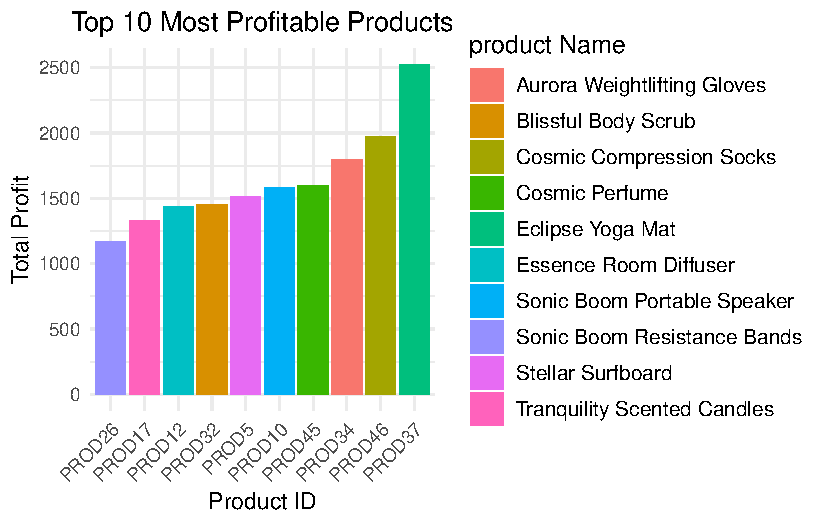
\includegraphics{Report_files/figure-pdf/unnamed-chunk-26-1.pdf}

}

\end{figure}

\begin{Shaded}
\begin{Highlighting}[]
\CommentTok{\# Top Most Selling Products}

\CommentTok{\# Creating a sales that that includes the total quantity sold for each product and selecting the top 10.}
\NormalTok{sales\_data }\OtherTok{\textless{}{-}}\NormalTok{ order\_item }\SpecialCharTok{\%\textgreater{}\%}
  \FunctionTok{group\_by}\NormalTok{(product\_id) }\SpecialCharTok{\%\textgreater{}\%}
  \FunctionTok{summarise}\NormalTok{(}\AttributeTok{Total\_Sales =} \FunctionTok{sum}\NormalTok{(order\_quantity, }\AttributeTok{na.rm =} \ConstantTok{TRUE}\NormalTok{)) }\SpecialCharTok{\%\textgreater{}\%}
  \FunctionTok{arrange}\NormalTok{(}\FunctionTok{desc}\NormalTok{(Total\_Sales))}

\NormalTok{top\_selling\_products }\OtherTok{\textless{}{-}}\NormalTok{ sales\_data }\SpecialCharTok{\%\textgreater{}\%}
  \FunctionTok{left\_join}\NormalTok{(product, }\AttributeTok{by =} \StringTok{"product\_id"}\NormalTok{) }\SpecialCharTok{\%\textgreater{}\%}
  \FunctionTok{select}\NormalTok{(product\_id, product\_name, Total\_Sales) }\SpecialCharTok{\%\textgreater{}\%}
  \FunctionTok{top\_n}\NormalTok{(}\DecValTok{10}\NormalTok{, Total\_Sales)}

\CommentTok{\# Visualizing the results}
\FunctionTok{ggplot}\NormalTok{(top\_selling\_products, }\FunctionTok{aes}\NormalTok{(}\AttributeTok{x =} \FunctionTok{reorder}\NormalTok{(product\_id, Total\_Sales), }\AttributeTok{y =}\NormalTok{ Total\_Sales, }\AttributeTok{fill =}\NormalTok{ product\_name)) }\SpecialCharTok{+}
  \FunctionTok{geom\_bar}\NormalTok{(}\AttributeTok{stat =} \StringTok{"identity"}\NormalTok{) }\SpecialCharTok{+}
  \FunctionTok{scale\_fill\_discrete}\NormalTok{(}\AttributeTok{name =} \StringTok{"product Name"}\NormalTok{) }\SpecialCharTok{+} 
  \FunctionTok{labs}\NormalTok{(}\AttributeTok{title =} \StringTok{"Top Most Selling Products"}\NormalTok{, }\AttributeTok{x =} \StringTok{"Product ID"}\NormalTok{, }\AttributeTok{y =} \StringTok{"Total Sales"}\NormalTok{) }\SpecialCharTok{+}
  \FunctionTok{theme\_minimal}\NormalTok{() }\SpecialCharTok{+}
  \FunctionTok{theme}\NormalTok{(}\AttributeTok{axis.text.x =} \FunctionTok{element\_text}\NormalTok{(}\AttributeTok{angle =} \DecValTok{45}\NormalTok{, }\AttributeTok{hjust =} \DecValTok{1}\NormalTok{),}
        \AttributeTok{legend.title =} \FunctionTok{element\_text}\NormalTok{(}\AttributeTok{size =} \DecValTok{12}\NormalTok{), }
        \AttributeTok{legend.text =} \FunctionTok{element\_text}\NormalTok{(}\AttributeTok{size =} \DecValTok{10}\NormalTok{), }
        \AttributeTok{plot.title =} \FunctionTok{element\_text}\NormalTok{(}\AttributeTok{hjust =} \FloatTok{0.5}\NormalTok{))}
\end{Highlighting}
\end{Shaded}

\begin{figure}[H]

{\centering 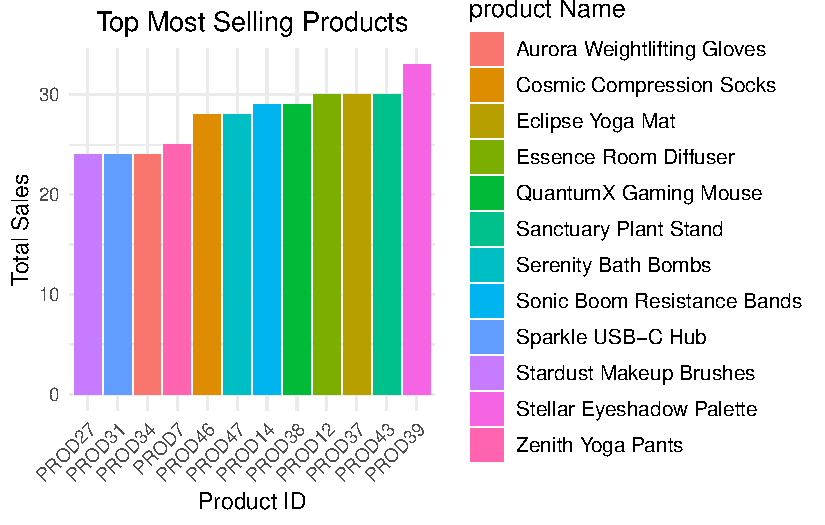
\includegraphics{Report_files/figure-pdf/unnamed-chunk-26-2.pdf}

}

\end{figure}

\begin{Shaded}
\begin{Highlighting}[]
\CommentTok{\#Report 2}

\CommentTok{\# Bundles vs Individual products Comparison by Sales Volume}

\CommentTok{\# Join product with order item }
\NormalTok{product\_order\_item }\OtherTok{\textless{}{-}}\NormalTok{ order\_item }\SpecialCharTok{\%\textgreater{}\%}
  \FunctionTok{inner\_join}\NormalTok{(product, }\AttributeTok{by =} \StringTok{"product\_id"}\NormalTok{)}

\CommentTok{\# Calculate total quantity sold for bundled products}
\NormalTok{bundled\_sales }\OtherTok{\textless{}{-}}\NormalTok{ product\_order\_item }\SpecialCharTok{\%\textgreater{}\%}
  \FunctionTok{filter}\NormalTok{(}\SpecialCharTok{!}\FunctionTok{is.na}\NormalTok{(main\_product\_id)) }\SpecialCharTok{\%\textgreater{}\%}
  \FunctionTok{group\_by}\NormalTok{(main\_product\_id) }\SpecialCharTok{\%\textgreater{}\%}
  \FunctionTok{summarise}\NormalTok{(}\AttributeTok{Total\_Quantity\_Sold =} \FunctionTok{sum}\NormalTok{(order\_quantity, }\AttributeTok{na.rm =} \ConstantTok{TRUE}\NormalTok{)) }\SpecialCharTok{\%\textgreater{}\%}
  \FunctionTok{ungroup}\NormalTok{() }\SpecialCharTok{\%\textgreater{}\%}
  \FunctionTok{mutate}\NormalTok{(}\AttributeTok{Product\_Type =} \StringTok{"Bundled"}\NormalTok{)}

\CommentTok{\# Calculate total quantity sold for individual products}
\NormalTok{individual\_sales }\OtherTok{\textless{}{-}}\NormalTok{ product\_order\_item }\SpecialCharTok{\%\textgreater{}\%}
  \FunctionTok{filter}\NormalTok{(}\FunctionTok{is.na}\NormalTok{(main\_product\_id)) }\SpecialCharTok{\%\textgreater{}\%}
  \FunctionTok{group\_by}\NormalTok{(product\_id) }\SpecialCharTok{\%\textgreater{}\%}
  \FunctionTok{summarise}\NormalTok{(}\AttributeTok{Total\_Quantity\_Sold =} \FunctionTok{sum}\NormalTok{(order\_quantity, }\AttributeTok{na.rm =} \ConstantTok{TRUE}\NormalTok{)) }\SpecialCharTok{\%\textgreater{}\%}
  \FunctionTok{ungroup}\NormalTok{() }\SpecialCharTok{\%\textgreater{}\%}
  \FunctionTok{mutate}\NormalTok{(}\AttributeTok{Product\_Type =} \StringTok{"Individual"}\NormalTok{)}

\CommentTok{\# Combining the results}
\NormalTok{total\_sales\_by\_type }\OtherTok{\textless{}{-}} \FunctionTok{bind\_rows}\NormalTok{(bundled\_sales, individual\_sales) }\SpecialCharTok{\%\textgreater{}\%}
  \FunctionTok{group\_by}\NormalTok{(Product\_Type) }\SpecialCharTok{\%\textgreater{}\%}
  \FunctionTok{summarise}\NormalTok{(}\AttributeTok{Total\_Quantity\_Sold =} \FunctionTok{sum}\NormalTok{(Total\_Quantity\_Sold, }\AttributeTok{na.rm =} \ConstantTok{TRUE}\NormalTok{)) }\SpecialCharTok{\%\textgreater{}\%}
  \FunctionTok{ungroup}\NormalTok{()}

\FunctionTok{print}\NormalTok{(total\_sales\_by\_type)}
\end{Highlighting}
\end{Shaded}

\begin{verbatim}
# A tibble: 2 x 2
  Product_Type Total_Quantity_Sold
  <chr>                      <int>
1 Bundled                      501
2 Individual                   463
\end{verbatim}

\begin{Shaded}
\begin{Highlighting}[]
\CommentTok{\# Visualizing the results}
\FunctionTok{ggplot}\NormalTok{(total\_sales\_by\_type, }\FunctionTok{aes}\NormalTok{(}\AttributeTok{x =}\NormalTok{ Product\_Type, }\AttributeTok{y =}\NormalTok{ Total\_Quantity\_Sold, }\AttributeTok{fill =}\NormalTok{ Product\_Type)) }\SpecialCharTok{+}
  \FunctionTok{geom\_bar}\NormalTok{(}\AttributeTok{stat =} \StringTok{"identity"}\NormalTok{, }\AttributeTok{width =} \FloatTok{0.5}\NormalTok{) }\SpecialCharTok{+}  \CommentTok{\# Adjust width here}
  \FunctionTok{scale\_fill\_manual}\NormalTok{(}\AttributeTok{values =} \FunctionTok{c}\NormalTok{(}\StringTok{"Bundled"} \OtherTok{=} \StringTok{"skyblue"}\NormalTok{, }\StringTok{"Individual"} \OtherTok{=} \StringTok{"salmon"}\NormalTok{)) }\SpecialCharTok{+}
  \FunctionTok{labs}\NormalTok{(}\AttributeTok{title =} \StringTok{"Total Quantity Sold by Product Type"}\NormalTok{,}
       \AttributeTok{x =} \StringTok{"Product Type"}\NormalTok{,}
       \AttributeTok{y =} \StringTok{"Total Quantity Sold"}\NormalTok{) }\SpecialCharTok{+}
  \FunctionTok{theme\_minimal}\NormalTok{() }\SpecialCharTok{+}
  \FunctionTok{theme}\NormalTok{(}\AttributeTok{legend.position =} \StringTok{"none"}\NormalTok{) }
\end{Highlighting}
\end{Shaded}

\begin{figure}[H]

{\centering 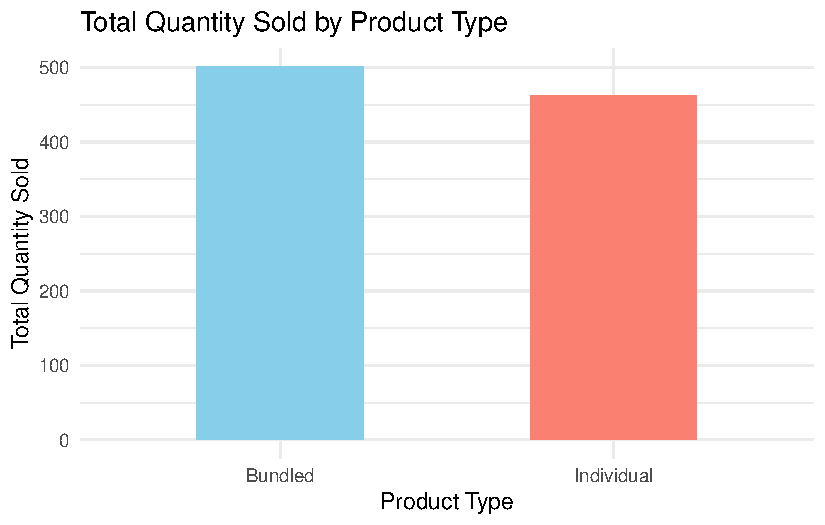
\includegraphics{Report_files/figure-pdf/unnamed-chunk-27-1.pdf}

}

\end{figure}

\begin{Shaded}
\begin{Highlighting}[]
\CommentTok{\#SQL Query to get the sales over a time period }

\NormalTok{time\_period\_sales}\OtherTok{\textless{}{-}}\NormalTok{ RSQLite}\SpecialCharTok{::}\FunctionTok{dbGetQuery}\NormalTok{(connect,}\StringTok{\textquotesingle{}SELECT ORDITM.order\_id, order\_quantity,order\_date FROM ORDER\_DETAIL ORDDET INNER JOIN ORDER\_ITEM ORDITM ON ORDITM.order\_id = ORDDET.order\_id\textquotesingle{}}\NormalTok{)}
\CommentTok{\#test}

\CommentTok{\#Conversion of order\_date field to appropiate format}
\NormalTok{time\_period\_sales}\SpecialCharTok{$}\NormalTok{order\_date }\OtherTok{\textless{}{-}} \FunctionTok{as.Date}\NormalTok{(time\_period\_sales}\SpecialCharTok{$}\NormalTok{order\_date, }\AttributeTok{format=}\StringTok{"\%d/\%m/\%Y"}\NormalTok{)}

\NormalTok{time\_period\_sales}\SpecialCharTok{$}\NormalTok{order\_date\_mnth\_yr }\OtherTok{\textless{}{-}} \FunctionTok{format}\NormalTok{(time\_period\_sales}\SpecialCharTok{$}\NormalTok{order\_date,}\StringTok{\textquotesingle{}\%Y/\%m\textquotesingle{}}\NormalTok{)}

\CommentTok{\#Conversion of order\_date field to factors with levels}

\NormalTok{time\_period\_sales}\SpecialCharTok{$}\NormalTok{order\_date\_mnth\_yr }\OtherTok{\textless{}{-}} \FunctionTok{factor}\NormalTok{(time\_period\_sales}\SpecialCharTok{$}\NormalTok{order\_date\_mnth\_yr, }\AttributeTok{levels=}\FunctionTok{c}\NormalTok{(}\StringTok{\textquotesingle{}2022/06\textquotesingle{}}\NormalTok{,}\StringTok{\textquotesingle{}2022/07\textquotesingle{}}\NormalTok{,}\StringTok{\textquotesingle{}2022/08\textquotesingle{}}\NormalTok{,}\StringTok{\textquotesingle{}2022/09\textquotesingle{}}\NormalTok{,}\StringTok{\textquotesingle{}2022/10\textquotesingle{}}\NormalTok{,}\StringTok{\textquotesingle{}2022/11\textquotesingle{}}\NormalTok{,}\StringTok{\textquotesingle{}2022/12\textquotesingle{}}\NormalTok{,}\StringTok{\textquotesingle{}2023/01\textquotesingle{}}\NormalTok{,}\StringTok{\textquotesingle{}2023/02\textquotesingle{}}\NormalTok{,}\StringTok{\textquotesingle{}2023/03\textquotesingle{}}\NormalTok{,}\StringTok{\textquotesingle{}2023/04\textquotesingle{}}\NormalTok{,}\StringTok{\textquotesingle{}2023/05\textquotesingle{}}\NormalTok{,}\StringTok{\textquotesingle{}2023/06\textquotesingle{}}\NormalTok{,}\StringTok{\textquotesingle{}2023/07\textquotesingle{}}\NormalTok{,}\StringTok{\textquotesingle{}2023/08\textquotesingle{}}\NormalTok{,}\StringTok{\textquotesingle{}2023/09\textquotesingle{}}\NormalTok{,}\StringTok{\textquotesingle{}2023/10\textquotesingle{}}\NormalTok{,}\StringTok{\textquotesingle{}2023/11\textquotesingle{}}\NormalTok{,}\StringTok{\textquotesingle{}2023/12\textquotesingle{}}\NormalTok{))}

\CommentTok{\#Group by sales for each year}
\NormalTok{time\_period\_sales\_group\_by}\OtherTok{\textless{}{-}}\NormalTok{ time\_period\_sales }\SpecialCharTok{\%\textgreater{}\%} \FunctionTok{group\_by}\NormalTok{(order\_date\_mnth\_yr)}\SpecialCharTok{\%\textgreater{}\%}\FunctionTok{summarise}\NormalTok{(}\AttributeTok{quantity=}\FunctionTok{sum}\NormalTok{(order\_quantity))}

\CommentTok{\# Time series graph to show the quantity sold over a given time period}

\NormalTok{(}\FunctionTok{ggplot}\NormalTok{(time\_period\_sales\_group\_by, }\FunctionTok{aes}\NormalTok{(}\AttributeTok{x =}\NormalTok{ order\_date\_mnth\_yr, }\AttributeTok{y =}\NormalTok{ quantity,}\AttributeTok{group=}\DecValTok{1}\NormalTok{)) }\SpecialCharTok{+}  \FunctionTok{geom\_point}\NormalTok{()}\SpecialCharTok{+}\FunctionTok{geom\_line}\NormalTok{()}\SpecialCharTok{+}\FunctionTok{xlab}\NormalTok{(}\StringTok{\textquotesingle{}Time Period(year/month)\textquotesingle{}}\NormalTok{)}\SpecialCharTok{+}\FunctionTok{ylab}\NormalTok{(}\StringTok{\textquotesingle{}Quantity Sold\textquotesingle{}}\NormalTok{))}
\end{Highlighting}
\end{Shaded}

\begin{figure}[H]

{\centering 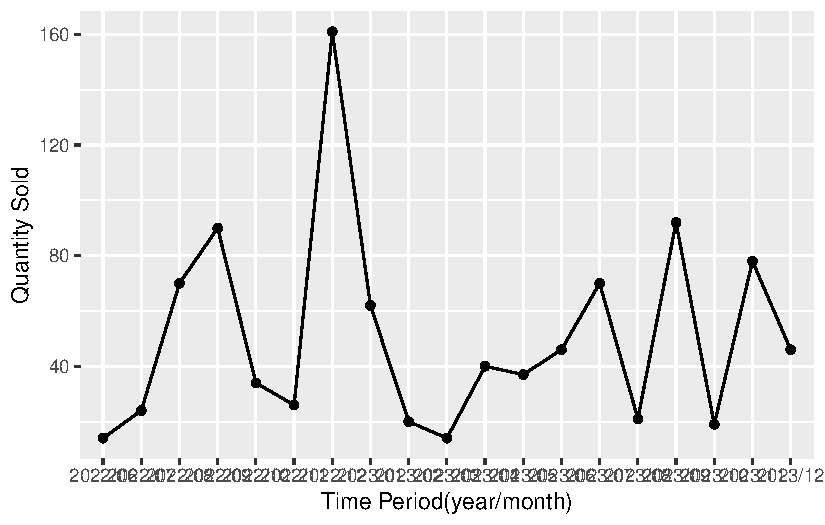
\includegraphics{Report_files/figure-pdf/Report 3-1.pdf}

}

\end{figure}

\begin{Shaded}
\begin{Highlighting}[]
\CommentTok{\#Report 4:}

\CommentTok{\#SQL query to join customer and order tables to get the sales for each city}

\NormalTok{cust\_order\_join}\OtherTok{\textless{}{-}}\NormalTok{ RSQLite}\SpecialCharTok{::}\FunctionTok{dbGetQuery}\NormalTok{(connect, }\StringTok{\textquotesingle{}SELECT city,ORDITM.order\_quantity FROM ADDRESS ADR INNER JOIN CUSTOMER CUST ON ADR.address\_id= CUST.address\_id INNER JOIN ORDER\_DETAIL ORDDET ON ORDDET.customer\_id = CUST.customer\_id INNER JOIN ORDER\_ITEM ORDITM ON ORDITM.order\_id = ORDDET.order\_id\textquotesingle{}}\NormalTok{)}

\CommentTok{\#cust\_order\_join\textless{}{-} inner\_join(Customer,Order,by="customer\_id")}

\CommentTok{\#Grouping by city to get the overall sales per city}

\NormalTok{sales\_per\_region}\OtherTok{\textless{}{-}}\NormalTok{ cust\_order\_join }\SpecialCharTok{\%\textgreater{}\%} \FunctionTok{group\_by}\NormalTok{(city)}\SpecialCharTok{\%\textgreater{}\%}\FunctionTok{summarise}\NormalTok{(}\AttributeTok{quantity=}\FunctionTok{sum}\NormalTok{(order\_quantity))}

\CommentTok{\#Get the top 10 cities for sales}
\NormalTok{top\_10\_sales\_per\_region }\OtherTok{\textless{}{-}}\NormalTok{ sales\_per\_region[}\FunctionTok{order}\NormalTok{(}\SpecialCharTok{{-}}\NormalTok{sales\_per\_region}\SpecialCharTok{$}\NormalTok{quantity),]}

\NormalTok{top\_10\_sales\_per\_region }\OtherTok{\textless{}{-}} \FunctionTok{head}\NormalTok{(top\_10\_sales\_per\_region,}\DecValTok{10}\NormalTok{)}

\CommentTok{\#Bar graph to show the sales per region}

\NormalTok{ggplot1 }\OtherTok{\textless{}{-}} \FunctionTok{ggplot}\NormalTok{(top\_10\_sales\_per\_region, }\FunctionTok{aes}\NormalTok{(}\AttributeTok{x =} \FunctionTok{reorder}\NormalTok{(city,}\SpecialCharTok{{-}}\NormalTok{quantity), }\AttributeTok{y =}\NormalTok{ quantity,}\AttributeTok{fill=}\NormalTok{quantity)) }\SpecialCharTok{+}  \FunctionTok{geom\_bar}\NormalTok{(}\AttributeTok{stat=}\StringTok{\textquotesingle{}identity\textquotesingle{}}\NormalTok{)}\SpecialCharTok{+}\FunctionTok{scale\_fill\_gradient}\NormalTok{(}\AttributeTok{low =} \StringTok{"lightblue"}\NormalTok{, }\AttributeTok{high =} \StringTok{"darkblue"}\NormalTok{)}\SpecialCharTok{+} \FunctionTok{xlab}\NormalTok{(}\StringTok{\textquotesingle{}Top 10 cities where sales is maximum\textquotesingle{}}\NormalTok{)}\SpecialCharTok{+}\FunctionTok{ylab}\NormalTok{(}\StringTok{\textquotesingle{}Quantity Sold\textquotesingle{}}\NormalTok{)}

\CommentTok{\#Table to get the revenue per city }

\NormalTok{cust\_order\_product\_join }\OtherTok{\textless{}{-}}\NormalTok{RSQLite}\SpecialCharTok{::}\FunctionTok{dbGetQuery}\NormalTok{(connect, }\StringTok{\textquotesingle{}SELECT city,ORDITM.order\_quantity,unit\_price FROM ADDRESS ADR INNER JOIN CUSTOMER CUST ON ADR.address\_id= CUST.address\_id INNER JOIN ORDER\_DETAIL ORDDET ON ORDDET.customer\_id = CUST.customer\_id INNER JOIN ORDER\_ITEM ORDITM ON ORDITM.order\_id = ORDDET.order\_id INNER JOIN PRODUCT PRD ON PRD.product\_id = ORDITM.product\_id\textquotesingle{}}\NormalTok{)}

\CommentTok{\#SQL Query to get the top 5 products}

\NormalTok{top\_5\_products }\OtherTok{\textless{}{-}}\NormalTok{RSQLite}\SpecialCharTok{::}\FunctionTok{dbGetQuery}\NormalTok{(connect, }\StringTok{\textquotesingle{}SELECT city,ORDITM.order\_quantity,unit\_price,PRD.product\_id,PRD.product\_name FROM ADDRESS ADR INNER JOIN CUSTOMER CUST ON ADR.address\_id= CUST.address\_id INNER JOIN ORDER\_DETAIL ORDDET ON ORDDET.customer\_id = CUST.customer\_id INNER JOIN ORDER\_ITEM ORDITM ON ORDITM.order\_id = ORDDET.order\_id INNER JOIN PRODUCT PRD ON PRD.product\_id = ORDITM.product\_id\textquotesingle{}}\NormalTok{)}

\CommentTok{\#Revenue calculation}

\NormalTok{cust\_order\_product\_join}\SpecialCharTok{$}\NormalTok{revenue }\OtherTok{\textless{}{-}}\NormalTok{  cust\_order\_product\_join}\SpecialCharTok{$}\NormalTok{order\_quantity}\SpecialCharTok{*}\NormalTok{cust\_order\_product\_join}\SpecialCharTok{$}\NormalTok{unit\_price}

\CommentTok{\#Grouping by the get the revenue for each city}
\NormalTok{revenue\_per\_region }\OtherTok{\textless{}{-}}\NormalTok{ cust\_order\_product\_join }\SpecialCharTok{\%\textgreater{}\%} \FunctionTok{group\_by}\NormalTok{(city) }\SpecialCharTok{\%\textgreater{}\%} \FunctionTok{summarise}\NormalTok{(}\AttributeTok{rev=} \FunctionTok{sum}\NormalTok{(revenue))}

\CommentTok{\#Get the top 10 cities for revenue}

\NormalTok{top\_5\_revenue\_per\_region }\OtherTok{\textless{}{-}}\NormalTok{ revenue\_per\_region[}\FunctionTok{order}\NormalTok{(}\SpecialCharTok{{-}}\NormalTok{revenue\_per\_region}\SpecialCharTok{$}\NormalTok{rev),]}

\NormalTok{top\_5\_revenue\_per\_region }\OtherTok{\textless{}{-}} \FunctionTok{head}\NormalTok{(top\_5\_revenue\_per\_region,}\DecValTok{10}\NormalTok{)}

\CommentTok{\#Bar graph to show the revenue per region}

\NormalTok{ggplot2 }\OtherTok{\textless{}{-}} \FunctionTok{ggplot}\NormalTok{(top\_5\_revenue\_per\_region, }\FunctionTok{aes}\NormalTok{(}\AttributeTok{x =} \FunctionTok{reorder}\NormalTok{(city, }\SpecialCharTok{{-}}\NormalTok{rev), }\AttributeTok{y =}\NormalTok{ rev,}\AttributeTok{fill=}\NormalTok{rev)) }\SpecialCharTok{+}  \FunctionTok{geom\_bar}\NormalTok{(}\AttributeTok{stat=}\StringTok{\textquotesingle{}identity\textquotesingle{}}\NormalTok{)}\SpecialCharTok{+}\FunctionTok{scale\_fill\_gradient}\NormalTok{(}\AttributeTok{low =} \StringTok{"lightblue"}\NormalTok{, }\AttributeTok{high =} \StringTok{"darkblue"}\NormalTok{)}\SpecialCharTok{+}\FunctionTok{xlab}\NormalTok{(}\StringTok{\textquotesingle{}Top 10 cities with the maximum revenue\textquotesingle{}}\NormalTok{)}\SpecialCharTok{+}\FunctionTok{ylab}\NormalTok{(}\StringTok{\textquotesingle{}Revenue\textquotesingle{}}\NormalTok{)}

\FunctionTok{grid.arrange}\NormalTok{(ggplot1,ggplot2)}
\end{Highlighting}
\end{Shaded}

\begin{figure}[H]

{\centering 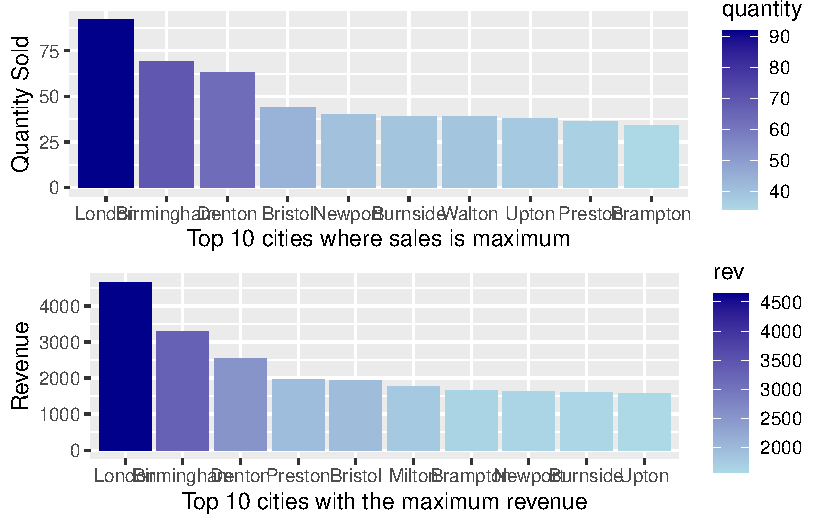
\includegraphics{Report_files/figure-pdf/unnamed-chunk-28-1.pdf}

}

\end{figure}

\begin{Shaded}
\begin{Highlighting}[]
\CommentTok{\#revenue\_per\_product\_region \textless{}{-} cust\_order\_product\_join \%\textgreater{}\% group\_by(city) \%\textgreater{}\% summarise(rev= sum(revenue))}

\CommentTok{\#Revenue calculation to show the top 5 products for each city with maximum revenue}

\NormalTok{top\_5\_products}\SpecialCharTok{$}\NormalTok{revenue }\OtherTok{\textless{}{-}}\NormalTok{ top\_5\_products}\SpecialCharTok{$}\NormalTok{order\_quantity}\SpecialCharTok{*}\NormalTok{top\_5\_products}\SpecialCharTok{$}\NormalTok{unit\_price}

\NormalTok{top\_5\_products\_region }\OtherTok{\textless{}{-}}\NormalTok{ top\_5\_products }\SpecialCharTok{\%\textgreater{}\%} \FunctionTok{group\_by}\NormalTok{(city,product\_name) }\SpecialCharTok{\%\textgreater{}\%} \FunctionTok{summarise}\NormalTok{(}\AttributeTok{rev=} \FunctionTok{sum}\NormalTok{(revenue))}
\end{Highlighting}
\end{Shaded}

\begin{verbatim}
`summarise()` has grouped output by 'city'. You can override using the
`.groups` argument.
\end{verbatim}

\begin{Shaded}
\begin{Highlighting}[]
\CommentTok{\#Table to show the products that are sold for the top 2 revenue producing cities}
\NormalTok{(top\_5\_products\_region }\OtherTok{\textless{}{-}}\NormalTok{ top\_5\_products\_region }\SpecialCharTok{\%\textgreater{}\%} \FunctionTok{filter}\NormalTok{(city }\SpecialCharTok{\%in\%} \FunctionTok{head}\NormalTok{(top\_5\_revenue\_per\_region}\SpecialCharTok{$}\NormalTok{city,}\DecValTok{2}\NormalTok{)) }\SpecialCharTok{\%\textgreater{}\%} \FunctionTok{select}\NormalTok{(product\_name))}
\end{Highlighting}
\end{Shaded}

\begin{verbatim}
Adding missing grouping variables: `city`
\end{verbatim}

\begin{verbatim}
# A tibble: 24 x 2
# Groups:   city [2]
   city       product_name               
   <chr>      <chr>                      
 1 Birmingham Cosmic Compression Socks   
 2 Birmingham Essence Room Diffuser      
 3 Birmingham FusionX Gaming Console     
 4 Birmingham Moonbeam Cardigan          
 5 Birmingham Nebula Scarf               
 6 Birmingham Solar Flare Sweater        
 7 Birmingham Sonic Boom Portable Speaker
 8 Birmingham Sonic Boom Resistance Bands
 9 Birmingham Stellar Eyeshadow Palette  
10 Birmingham Tranquility Scented Candles
# i 14 more rows
\end{verbatim}

\begin{Shaded}
\begin{Highlighting}[]
\CommentTok{\#Report 5}
\CommentTok{\# Joining Product with advertise\_in and advertisement to get advertisement details}
\NormalTok{advertise\_in }\OtherTok{\textless{}{-}}\NormalTok{ RSQLite}\SpecialCharTok{::}\FunctionTok{dbGetQuery}\NormalTok{(connect,}\StringTok{\textquotesingle{}SELECT * FROM ADVERTISE\_IN\textquotesingle{}}\NormalTok{)}
\NormalTok{advertisement }\OtherTok{\textless{}{-}}\NormalTok{ RSQLite}\SpecialCharTok{::}\FunctionTok{dbGetQuery}\NormalTok{(connect,}\StringTok{\textquotesingle{}SELECT * FROM ADVERTISEMENT\textquotesingle{}}\NormalTok{)}

\NormalTok{advertisement\_data }\OtherTok{\textless{}{-}}\NormalTok{ product }\SpecialCharTok{\%\textgreater{}\%}
  \FunctionTok{inner\_join}\NormalTok{(advertise\_in, }\AttributeTok{by =} \StringTok{"product\_id"}\NormalTok{) }\SpecialCharTok{\%\textgreater{}\%}
  \FunctionTok{inner\_join}\NormalTok{(advertisement, }\AttributeTok{by =} \StringTok{"ad\_id"}\NormalTok{) }\SpecialCharTok{\%\textgreater{}\%}
  \FunctionTok{group\_by}\NormalTok{(product\_id, product\_name, ad\_place) }\SpecialCharTok{\%\textgreater{}\%}
  \FunctionTok{summarise}\NormalTok{(}
    \AttributeTok{total\_frequency =} \FunctionTok{sum}\NormalTok{(ad\_frequency), }\CommentTok{\# Sum the total frequency of ads for each ad place}
    \AttributeTok{.groups =} \StringTok{\textquotesingle{}drop\textquotesingle{}}\NormalTok{ )}


\CommentTok{\# Joining product with order to get the number of sales per product}
\NormalTok{number\_of\_sales }\OtherTok{\textless{}{-}}\NormalTok{ product }\SpecialCharTok{\%\textgreater{}\%}
  \FunctionTok{inner\_join}\NormalTok{(order\_item, }\AttributeTok{by =} \StringTok{"product\_id"}\NormalTok{) }\SpecialCharTok{\%\textgreater{}\%}
  \FunctionTok{group\_by}\NormalTok{(product\_id, product\_name) }\SpecialCharTok{\%\textgreater{}\%}
  \FunctionTok{summarise}\NormalTok{(}\AttributeTok{sales\_count =} \FunctionTok{n}\NormalTok{(), }\AttributeTok{.groups =} \StringTok{\textquotesingle{}drop\textquotesingle{}}\NormalTok{)}



\NormalTok{merged\_data }\OtherTok{\textless{}{-}} \FunctionTok{merge}\NormalTok{(number\_of\_sales, advertisement\_data, }\AttributeTok{by =} \FunctionTok{c}\NormalTok{(}\StringTok{"product\_id"}\NormalTok{, }\StringTok{"product\_name"}\NormalTok{))}



\CommentTok{\# Analyzing which ad place is most effective by calculating a ratio of total sales to total ad frequency}
\NormalTok{effective\_ad\_type }\OtherTok{\textless{}{-}}\NormalTok{ merged\_data }\SpecialCharTok{\%\textgreater{}\%}
  \FunctionTok{group\_by}\NormalTok{(ad\_place) }\SpecialCharTok{\%\textgreater{}\%}
  \FunctionTok{summarise}\NormalTok{( }\AttributeTok{total\_sales =} \FunctionTok{sum}\NormalTok{(sales\_count), }
             \AttributeTok{total\_frequency =} \FunctionTok{sum}\NormalTok{(total\_frequency), }\AttributeTok{.groups =} \StringTok{\textquotesingle{}drop\textquotesingle{}}\NormalTok{) }\SpecialCharTok{\%\textgreater{}\%}
  \FunctionTok{mutate}\NormalTok{( }\AttributeTok{effectiveness =}\NormalTok{ total\_sales }\SpecialCharTok{/}\NormalTok{ total\_frequency) }\SpecialCharTok{\%\textgreater{}\%}
  \FunctionTok{arrange}\NormalTok{(}\FunctionTok{desc}\NormalTok{(effectiveness))}




\FunctionTok{ggplot}\NormalTok{(effective\_ad\_type, }\FunctionTok{aes}\NormalTok{(}\AttributeTok{x =}\NormalTok{ ad\_place, }\AttributeTok{y =}\NormalTok{ effectiveness, }\AttributeTok{fill =}\NormalTok{ ad\_place)) }\SpecialCharTok{+}
  \FunctionTok{geom\_col}\NormalTok{(}\AttributeTok{show.legend =} \ConstantTok{FALSE}\NormalTok{, }\AttributeTok{width =} \FloatTok{0.5}\NormalTok{) }\SpecialCharTok{+} \CommentTok{\# Adjust bar width here}
  \FunctionTok{scale\_fill\_brewer}\NormalTok{(}\AttributeTok{palette =} \StringTok{"Paired"}\NormalTok{) }\SpecialCharTok{+} \CommentTok{\# Use a more appealing color palette}
  \FunctionTok{labs}\NormalTok{(}\AttributeTok{title =} \StringTok{"Effectiveness of Advertisement Types"}\NormalTok{, }
       \AttributeTok{x =} \StringTok{"Ad Place"}\NormalTok{, }
       \AttributeTok{y =} \StringTok{"Total Sales / Total Frequency"}\NormalTok{) }\SpecialCharTok{+}
  \FunctionTok{theme\_minimal}\NormalTok{(}\AttributeTok{base\_size =} \DecValTok{14}\NormalTok{) }\SpecialCharTok{+} \CommentTok{\# Increase base text size for better readability}
  \FunctionTok{theme}\NormalTok{(}\AttributeTok{plot.title =} \FunctionTok{element\_text}\NormalTok{(}\AttributeTok{hjust =} \FloatTok{0.5}\NormalTok{, }\AttributeTok{size =} \DecValTok{20}\NormalTok{), }\CommentTok{\# Center and style title}
        \AttributeTok{axis.title =} \FunctionTok{element\_text}\NormalTok{(}\AttributeTok{size =} \DecValTok{16}\NormalTok{), }\CommentTok{\# Style axis titles}
        \AttributeTok{axis.text =} \FunctionTok{element\_text}\NormalTok{(}\AttributeTok{size =} \DecValTok{12}\NormalTok{), }\CommentTok{\# Style axis texts}
        \AttributeTok{panel.grid.major =} \FunctionTok{element\_blank}\NormalTok{(), }\CommentTok{\# Remove major grid lines}
        \AttributeTok{panel.grid.minor =} \FunctionTok{element\_blank}\NormalTok{(), }\CommentTok{\# Remove minor grid lines}
        \AttributeTok{panel.background =} \FunctionTok{element\_rect}\NormalTok{(}\AttributeTok{fill =} \StringTok{"white"}\NormalTok{, }\AttributeTok{colour =} \StringTok{"grey50"}\NormalTok{)) }\CommentTok{\# Style panel background}
\end{Highlighting}
\end{Shaded}

\begin{figure}[H]

{\centering 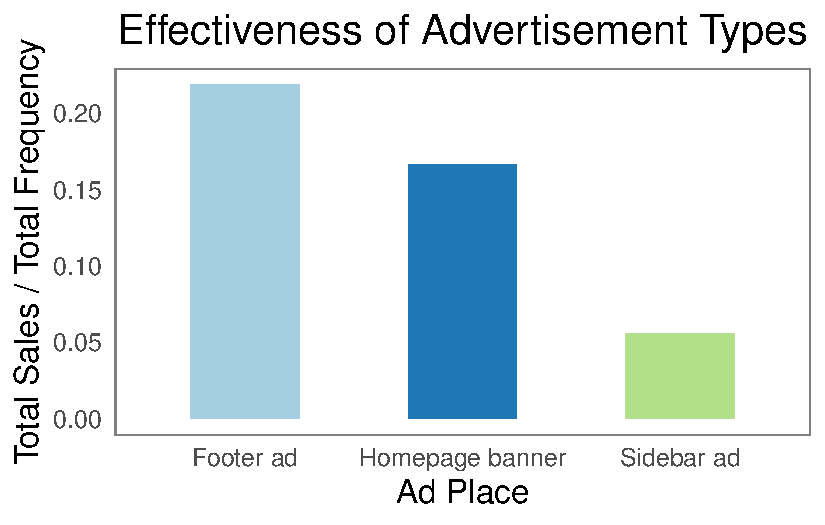
\includegraphics{Report_files/figure-pdf/unnamed-chunk-29-1.pdf}

}

\end{figure}

\begin{Shaded}
\begin{Highlighting}[]
\CommentTok{\# \#Report 6}
\CommentTok{\# \#Calculating Marketplace fee}
\CommentTok{\# merged\_product\_fee \textless{}{-} product \%\textgreater{}\%}
\CommentTok{\#   inner\_join(select(category, category\_id, category\_fee, category\_name), by = "category\_id")}
\CommentTok{\# category\_fee \textless{}{-} order\_item \%\textgreater{}\%}
\CommentTok{\#   inner\_join(select(order\_detail, order\_id, order\_status), by = "order\_id") \%\textgreater{}\%}
\CommentTok{\#   inner\_join(select(merged\_product\_fee, product\_id, product\_name, unit\_price, category\_fee, category\_id, category\_name), by = "product\_id") \%\textgreater{}\%}
\CommentTok{\#   filter(order\_status == "Completed") \%\textgreater{}\%}
\CommentTok{\#   mutate(marketplace\_fee = order\_quantity * unit\_price * category\_fee/100) \%\textgreater{}\%}
\CommentTok{\#   mutate(cat\_total\_sales = order\_quantity * unit\_price) \%\textgreater{}\%}
\CommentTok{\#   group\_by(category\_id, category\_name) \%\textgreater{}\%}
\CommentTok{\#   summarise(total\_fee = sum(marketplace\_fee), total\_sales = sum(cat\_total\_sales), total\_sales\_unit = sum(order\_quantity)) \%\textgreater{}\% inner\_join(select(category\_id, Average\_Rating), by= \textquotesingle{}category\_id\textquotesingle{})}
\CommentTok{\# }
\CommentTok{\# }
\CommentTok{\# \#Visualise}
\CommentTok{\# }
\CommentTok{\# }
\CommentTok{\# \#Graph to compare Category sales VS Category Fee}
\CommentTok{\# ggplot(category\_fee, aes(x = reorder(category\_name, {-}total\_fee))) +}
\CommentTok{\#   geom\_bar(aes(y = total\_sales, fill = "Total Sales"), stat = "identity", position = position\_dodge(width = 0.9), alpha = 0.7) +}
\CommentTok{\#   geom\_bar(aes(y = total\_fee, fill = "Marketplace Fee"), stat = "identity", position = position\_dodge(width = 0.9)) +}
\CommentTok{\#   scale\_fill\_manual(name = "Category", values = c("Marketplace Fee" = "\#3182bd", "Total Sales" = "\#31a354")) +}
\CommentTok{\#   labs(title = "Marketplace Fee vs Total Sales by Category", x = "Category", y = "Amount, USD") +}
\CommentTok{\#   theme\_minimal() +}
\CommentTok{\#   theme(axis.text.x = element\_text(angle = 45, hjust = 1))}
\end{Highlighting}
\end{Shaded}

\begin{Shaded}
\begin{Highlighting}[]
\CommentTok{\# \#Report 7}
\CommentTok{\# \# Graph to compare Category sales VS Category average rating}
\CommentTok{\# ggplot(category\_fee, aes(x = reorder(category\_name, {-}Average\_Rating))) +}
\CommentTok{\#   geom\_bar(aes(y = total\_sales\_unit, fill = "Total Sales in Units"), stat = "identity", position = position\_dodge(width = 0.9), alpha = 0.6) +}
\CommentTok{\#   geom\_bar(aes(y = (Average\_Rating{-}3)*20, fill = "Average Rating"), stat = "identity", position = position\_dodge(width = 0.9), alpha = 1) +}
\CommentTok{\#   geom\_text(aes(label = sprintf("\%.2f", Average\_Rating), y = Average\_Rating, x = category\_name), }
\CommentTok{\#             color = "black", size = 4, hjust = 0.5) +}
\CommentTok{\#   scale\_fill\_manual(name = "Category", values = c("Average Rating" = "\#FFCC80", "Total Sales in Units" = "\#31a354")) +}
\CommentTok{\#   labs(title = "Average Rating vs Total Sales in Units by Category", x = "Category", y = "Total Sales in Units") +}
\CommentTok{\#   theme\_minimal() +}
\CommentTok{\#   theme(axis.text.x = element\_text(angle = 45, hjust = 1)) +}
\CommentTok{\#   scale\_y\_continuous(name = "Total Sales in Units")}
\end{Highlighting}
\end{Shaded}

\hypertarget{task-4.2-comprehensive-reporting-with-quarto}{%
\subsubsection{Task 4.2: Comprehensive Reporting with
Quarto}\label{task-4.2-comprehensive-reporting-with-quarto}}

\textbf{Report 1: Profitability vs Popularity}

\begin{figure}

{\centering 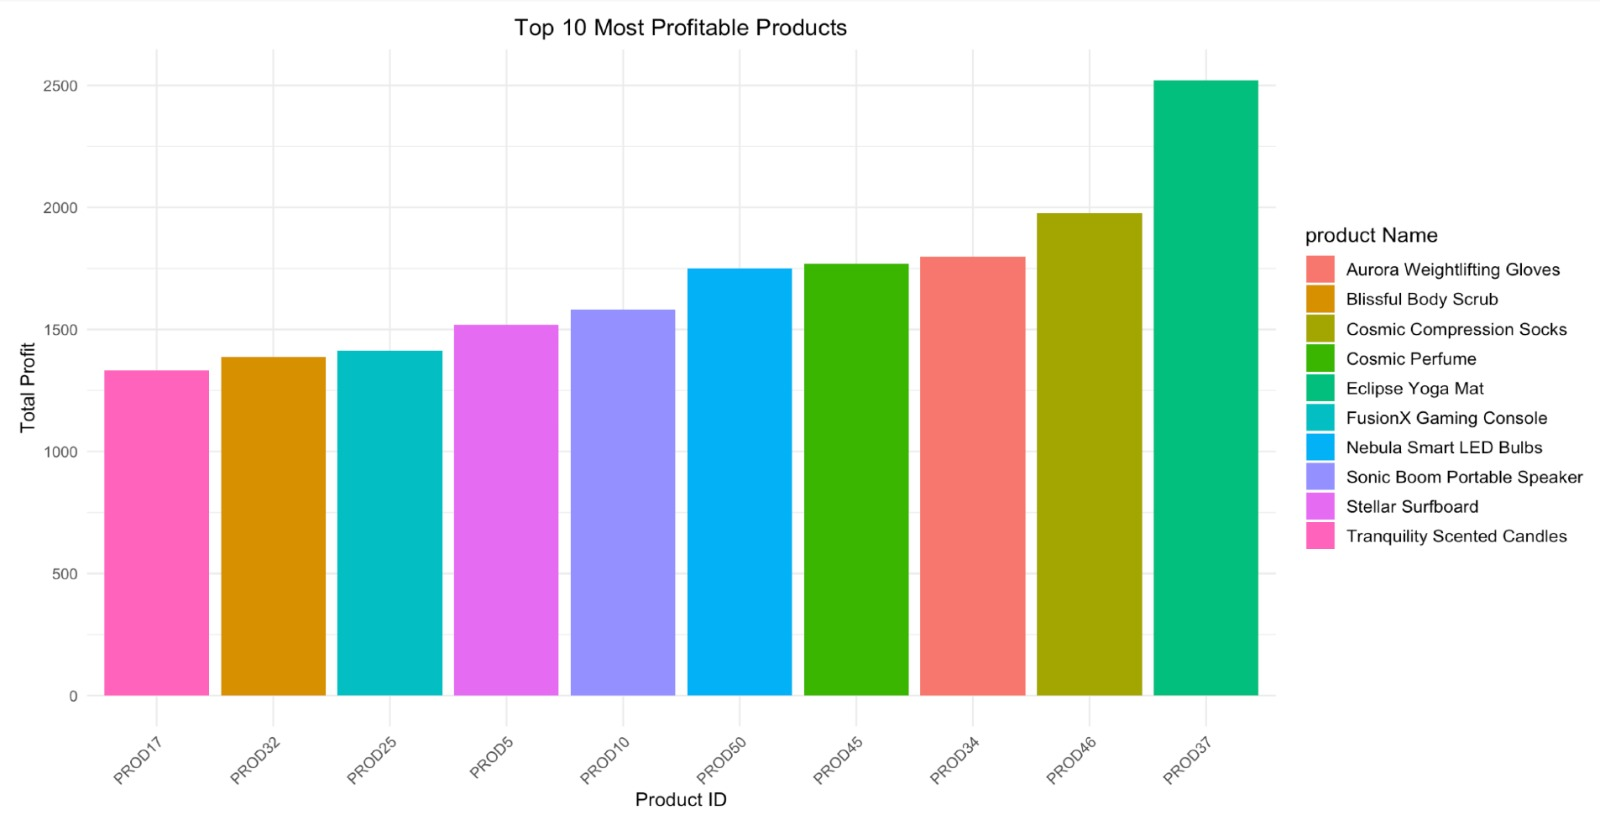
\includegraphics{images/Figure 1.jpeg}

}

\caption{Figure 1}

\end{figure}

\begin{figure}

{\centering 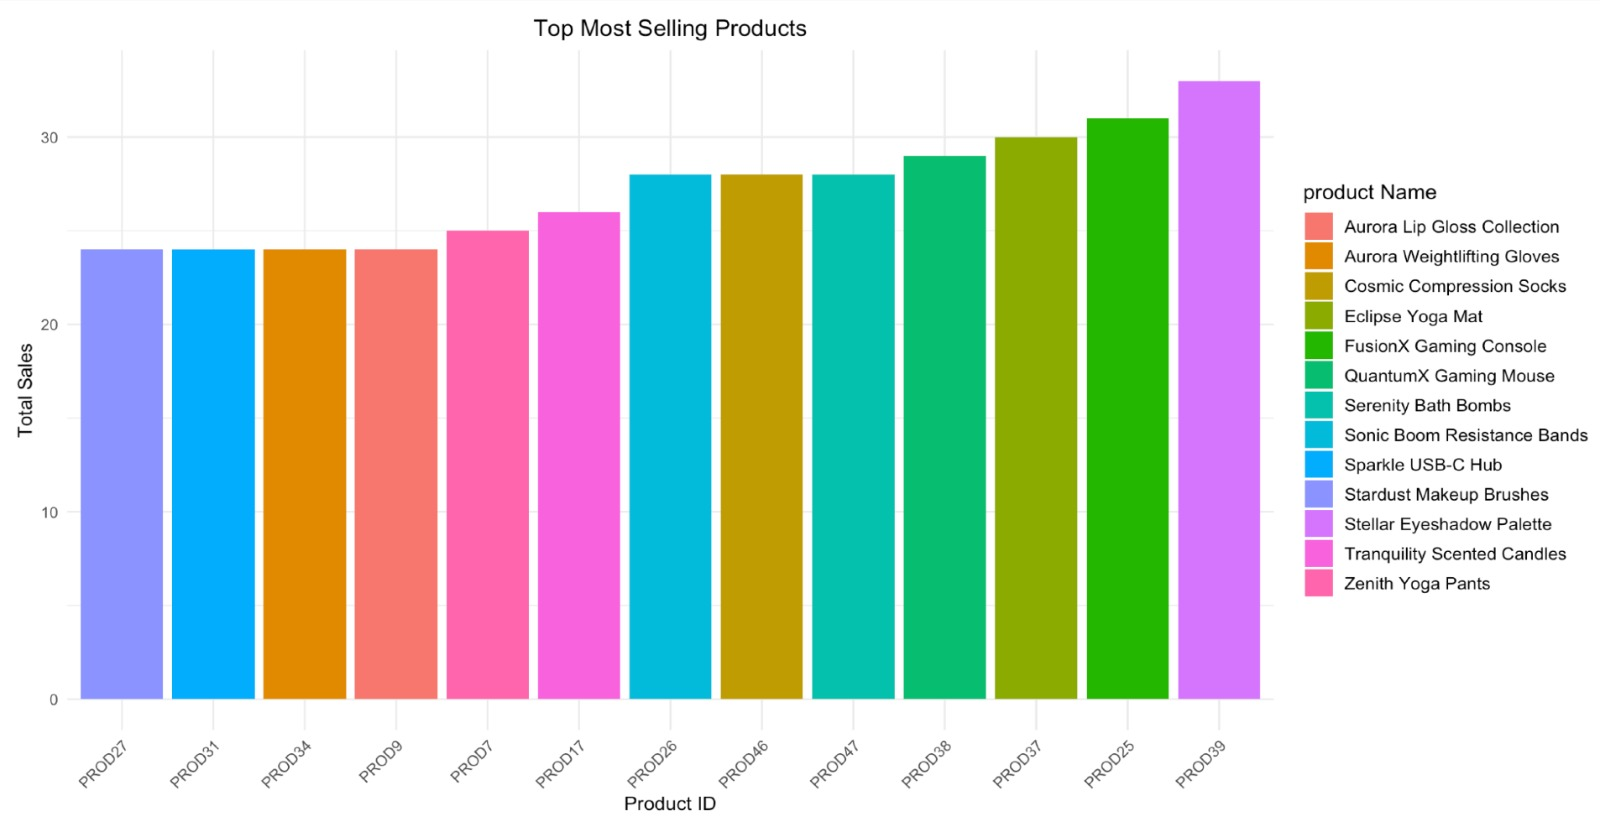
\includegraphics{images/Figure 2.jpeg}

}

\caption{Figure 2}

\end{figure}

Figure 1 represents the profitability of individual products sold by the
e-commerce company. The ``Eclipse Yoga Mat'' generates the highest
profit for the company among the assortment. This could indicate a
higher margin or a premium pricing strategy. Conversely, Figure 2
illustrates sales volume, where items like the ``Stellar Eyeshadow
Palette'' and ``Fusion X Gaming Console'' lead, suggesting they are
favored choices among consumers.

Some products, including the ``Aurora Weightlifting Gloves'', ``Cosmic
Compression Socks'' and ``Tranquility Scented Candles,'' appear in both
graphs, showcasing their strength in both popularity and profitability.
This dual presence is indicative of a successful product strategy by the
company. However, there are also noticeable discrepancies. For example,
``QuantumX Gaming Mouse'' appears as a top seller, yet it's absent from
the most profitable items, implying a lower profit margin. In contrast,
``Nebula Smart LED Bulbs'' are among the most profitable but not the top
sellers, suggesting a high margin compensating for lesser sales.

The e-commerce company could focus on marketing strategies for
high-margin products to boost their volume of sales, thus increasing
overall profitability. For products that sell well but are less
profitable, the company may need to assess whether they can improve
margins through better supplier negotiations.

Products that are both top sellers and highly profitable should be kept
in optimum stock to avoid lost sales opportunities. For less profitable
items, the company may consider keeping lower stock levels or even
discontinuing them if they do not contribute significantly to overall
profits.

\textbf{Report 2: Bundled vs Individual Products}

\begin{longtable}[]{@{}lr@{}}
\caption{\emph{Table 1}}\tabularnewline
\toprule\noalign{}
Product\_Type & Total\_Quantity\_Sold \\
\midrule\noalign{}
\endfirsthead
\toprule\noalign{}
Product\_Type & Total\_Quantity\_Sold \\
\midrule\noalign{}
\endhead
\bottomrule\noalign{}
\endlastfoot
Bundled & 491 \\
Individual & 499 \\
\end{longtable}

\begin{figure}

{\centering 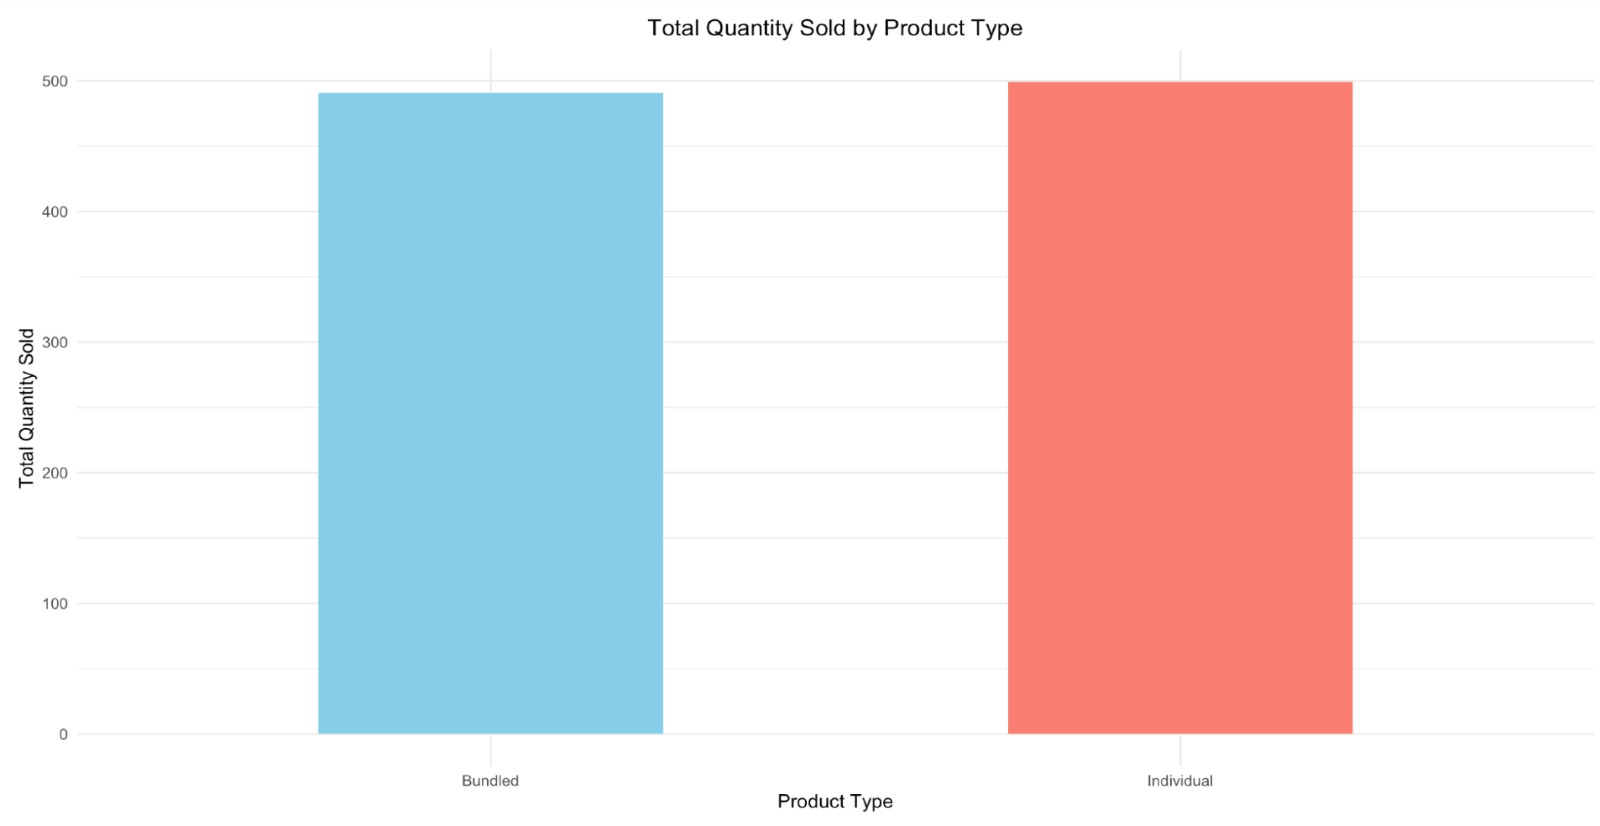
\includegraphics{images/Figure 3.jpeg}

}

\caption{Figure 3}

\end{figure}

As seen in Table 1, the total sales for individual products (products
sold without bundles) and bundled products yield nearly equal quantities
sold. Individual products slightly outperform bundled products (499 vs
491). This suggests that the e-commerce company's bundling strategy to
boost sales was not as effective as anticipated. However, it is
difficult to conclude the efficacy of this deal based solely on the
volume of sales.

Optimizing bundle offerings by analyzing and aligning them with customer
preferences, based on the average product ratings, can significantly
enhance their appeal. Experimenting with different bundle types and
conducting a cost-benefit analysis might uncover ways to refine the
strategy. The results (Figure 3) suggest a market demand for both types
of products, indicating that customers prefer some flexibility in their
buying options. Rather than discontinuing the bundle products, the
company should look deeper into the performance metrics of this deal
considering the inventory turnover and profit margins.

\textbf{Report 3: Sales Trend over the given time period}

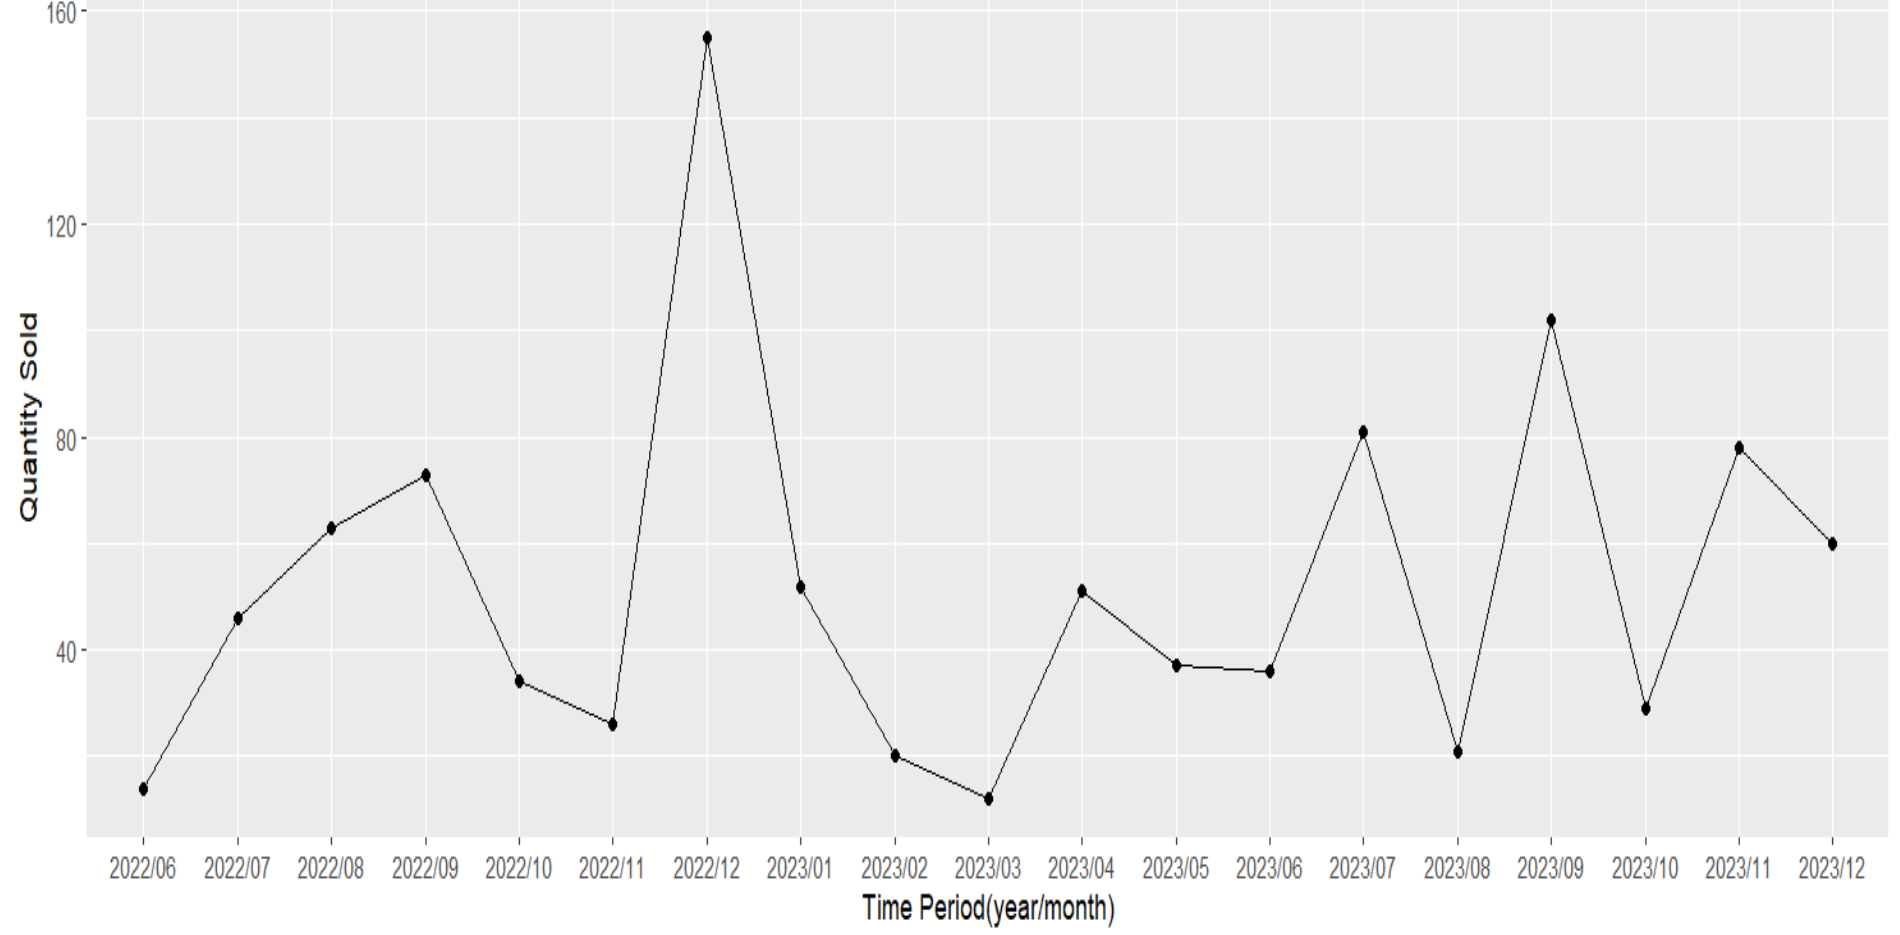
\includegraphics{images/Time Series Graph.png}

\emph{Figure 4: Time Series Graph to depict the seasonal trends in
sales}

Purchase pattern analysis is significant for an e-commerce company as
different strategies could be deployed to maximize sales and revenue.
Figure 4 illustrates that the sales was maximum at September and
December months over the time-period from 2022 to 2023. Hence
appropriate pricing strategies could be deployed to increase revenue
from top selling products. Also, a sharp decline in sales is identified
in October month which is later followed by an increase in succeeding
months. This study could help in an efficient inventory management in
place for perishable products. Overall, this variation in sales across
different seasons provides important insights for better management
decisions.

\textbf{Report 4: Comparison of sales and revenue for each city}

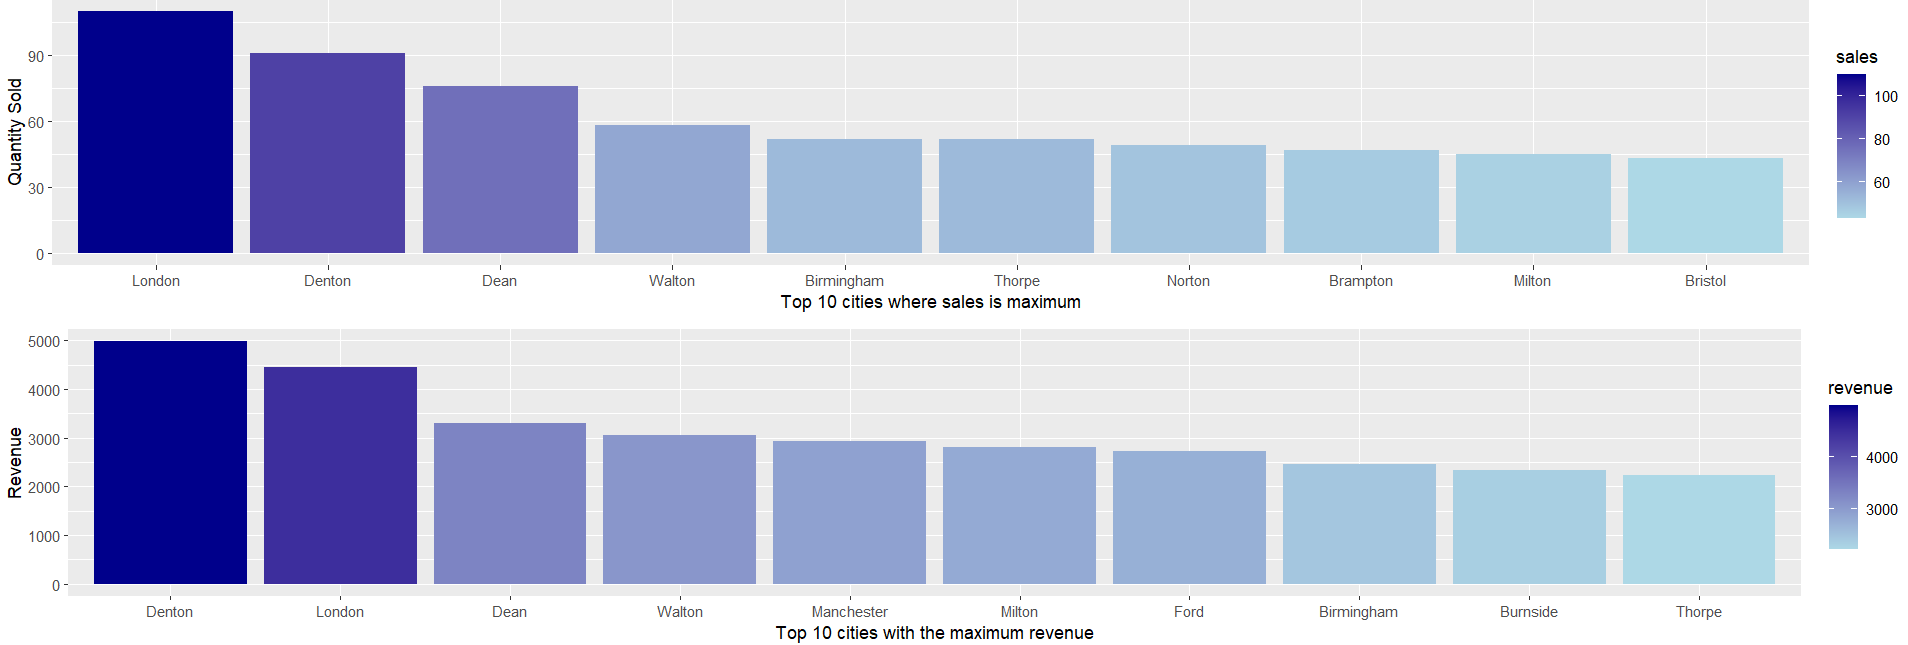
\includegraphics[width=7.61458in,height=4.04167in]{images/Revenue Graph.png}

\emph{Figure 5: Top 10 cities with maximum revenue and sales}

Figure 5 gives a crucial insight of cities that generated significant
revenue with lesser quantity of products sold. Top Products from these
cities could be identified as shown in table 1 as their sales could
improvise revenue to a great extent. Also, cities like Ford, Manchester
and Milton generated outstanding revenue even though their sales were
limited.

\textbf{Report 5: Analysis of Advertisement methods}

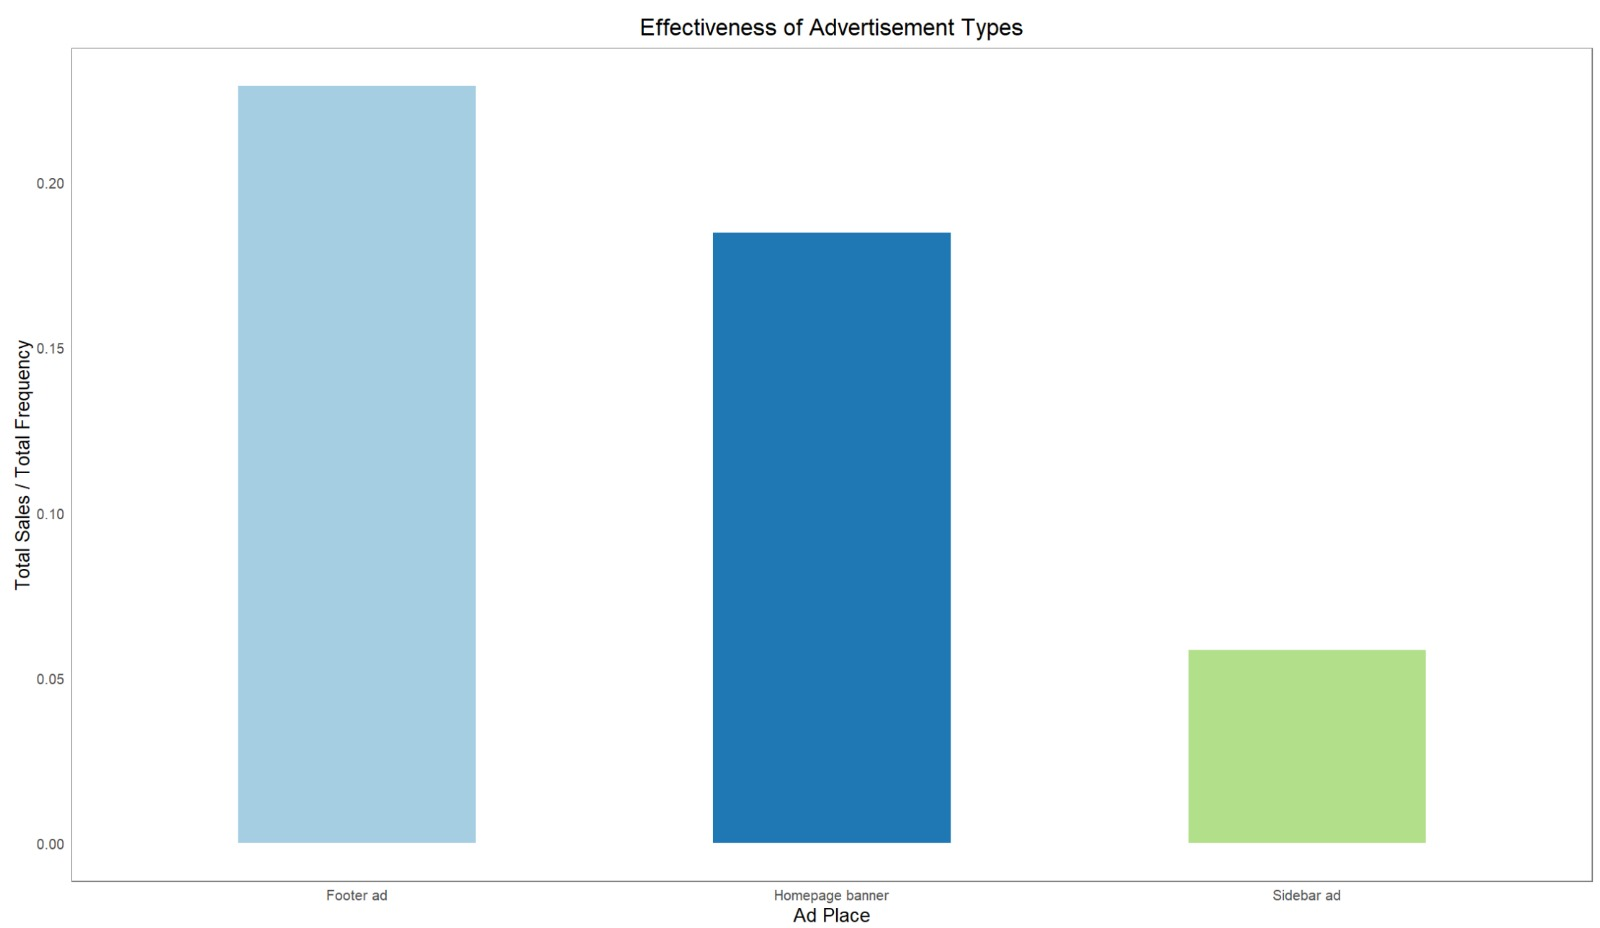
\includegraphics{images/Figure 4.jpeg}

\emph{Figure 6: Sales of products per 1 advertisement of each type}

We analysed 3 types of advertisements on the Marketplace to find that
Products that are advertised with the Figure 6 shows that Footer ads on
average have higher sales in units. The intention was to compare the
number of units sold depending on the type of advertisement this product
was in. This finding can be used to assign higher price for more
efficient advertisement types to be charged from suppliers.

\textbf{Report 6: Analysis of Marketplace transaction fees}

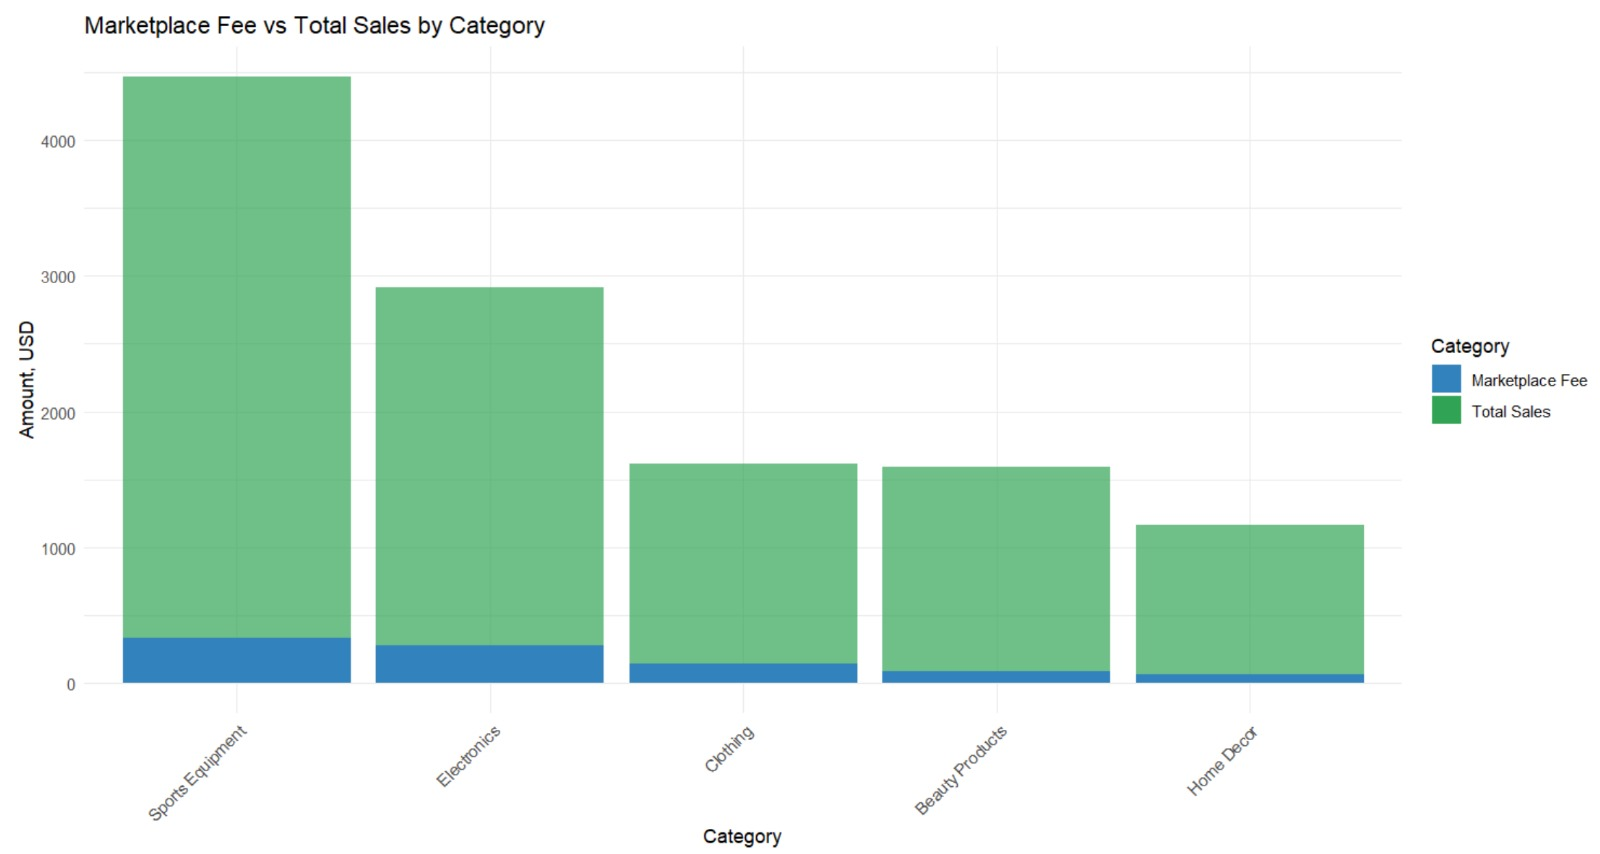
\includegraphics{images/Figure 5.jpeg}

\emph{Figure 7: Comparing Marketplace fees to the sales in each Category
of products}

The marketplace is the mediator between the customer and seller,
allowing convenience for both. This service is not free. Sellers pay
fees for each transaction. These fees and advertisements make the
marketplace profit. The fee varies depending on the category of goods.
We compared the combined amount of fees for each sold item by category
to find out which category brings the Marketplace more profit.

On Figure 7 we see that the higher the sales of the Category, the more
fees Marketplace earns on it. We consider increasing fees for the
categories with higher sales and decreasing fees for the categories with
low sales to maximise Marketplace profit by selling more in less popular
categories and getting higher fees for already popular ones. Sports
Equipment has the highest sales in terms of money, however, as we will
see later most units are sold in the Electronics category.

\textbf{Report 7: Analysis of Customers reviews on sales for each
category.}

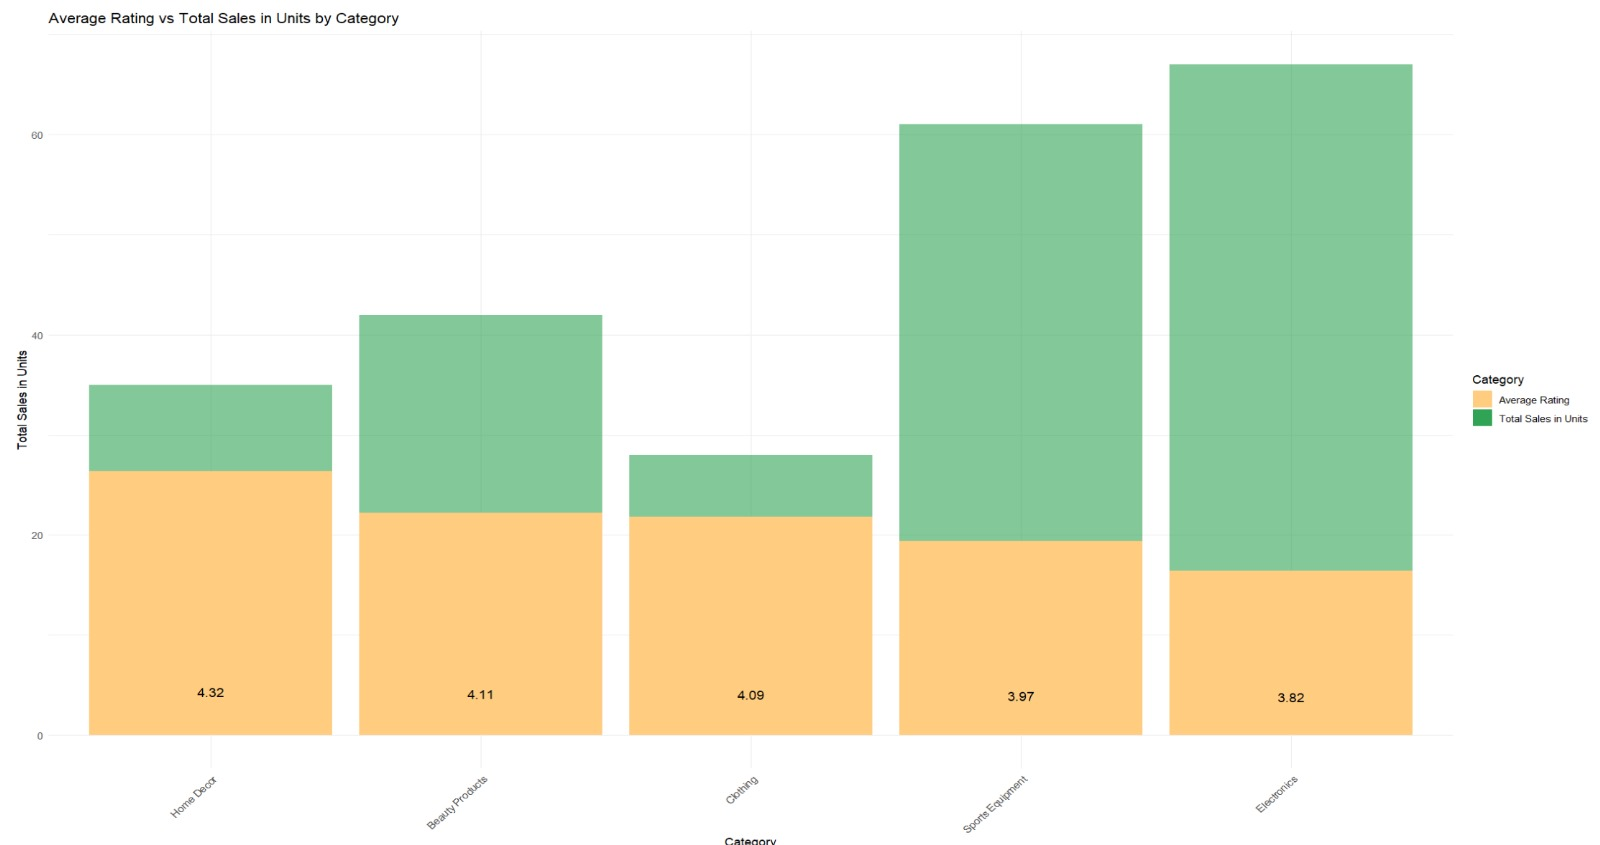
\includegraphics[width=8.65625in,height=\textheight]{images/Figure 6.jpeg}

\emph{Figure 8: Average customers' rating for the category and
category's sales in units}

It was found that categories that have products with higher ratings have
lower sales in units. This may appear wrong but most likely with the
increase in sales the number of negative reviews increases at a higher
rate. Marketplace may want to reconsider suppliers for the categories
with lower average ratings.



\end{document}
